\documentclass[10pt]{article}
\linespread{1.5}
% Language setting
\usepackage{polski}
\usepackage{amsfonts}
\usepackage{xurl}
\usepackage{float}
\usepackage{amssymb}
\usepackage{titlesec}
\usepackage{amsmath}
\usepackage{pdfpages}
\usepackage[utf8]{inputenc}
\newtheorem{Definicja}{Definition}[section]
\newtheorem{Twierdzenie}{Theorem}[section]
% Useful packages
\usepackage{algorithm}
\usepackage{algpseudocode}
\usepackage{amsmath}
\usepackage{bm}
\usepackage{graphicx}
\usepackage[polish, english]{babel}
\usepackage[colorlinks=true, allcolors=blue,  linkcolor = black]{hyperref}
\usepackage[nottoc,numbib]{tocbibind} 


\setcounter{secnumdepth}{4}
\titleformat{\paragraph}
{\normalfont\normalsize\bfseries}{\theparagraph}{1em}{}
\titlespacing*{\paragraph}
{0pt}{3.25ex plus 1ex minus .2ex}{1.5ex plus .2ex}

\makeatletter
\renewcommand{\ALG@name}{Algorytm}
\renewcommand{\listalgorithmname}{List of \ALG@name s}
\newcommand{\euler}{e}
\makeatother


\begin{document}

\begin{titlepage}

\includepdf{StronaTytulowa}
\end{titlepage}

\selectlanguage{english} 
\begin{abstract}
The main goal of this dissertation, which has been achieved, was to derive and prove equations, that lay out theoretical foundation for latent variable generative models. The equations for variational autoencoders, diffusion models and score models have been successfully derived. In the next step stochastic differential equations have been used, as a way to describe process, which perturbates data. Each model has been implemented in order too prove that equations work in practice. Source code which contains said implementations is available at \url{https://github.com/PiPower/GenerativeModels}
\end{abstract}

\textbf{\\ Keywords:} deep learning, probability theory, variational autoencoders, diffusion models, score models, stochastic differential equations.

\noindent
\textbf{\\Fields of Science and Technology in accordance with the requirements of the OECD:} 1.1 Mathematics

\newpage
\tableofcontents
\listoffigures
\newpage
\section{Introduction}
\subsection{Deep learning revolution}
Within last decade we have witnessed a great revolution in machine learning. Revolution has roughly started with"ImageNet Classification with Deep Convolutional Neural Networks" \cite{alexnet}, which described using GPUs for model training. Mentioned publication replaced sequentional model of execution used by CPU with parallel model of execution used by GPU(to be specific, GPU model is called SIMT by NVIDIA, more here\cite{gpu_guide}), with goal to increse general computation speed. This led for great increase in models' parameter count, count of used layers and allowed to use more complex operations 

Within years following, we have seen rise of many deep learning libraries using GPUs for computation, such as Tensorflow or Pytorch. One of the greatest successes of said libraries has been introduction of automatic differentiation into common use. This allowed to offload machine learning researchers from personally dealing with many complex problems in GPGPU programming or numerical methods. From that point onward deep learning research picked up the pace. Libraries such as Tensorflow or Pytorch have highly increased popularity of deep learning which has led to many breakthroughs within last decade.

At the time of writing this publication progress in deep learning is gaining attention from wider audience. NVIDIA DLSS  with certain quality compromises allows to highly increase framerate of computer games. chatGPT has become on of the fastest popularity gaining websites in history \cite{gpt_popularity}. The great progress of recent years has come with the cost. In recent years (at the time of writing this publication) we have seen problems of technical, legal, societal and moral. With increase of model sizes comes increase in needed computation. Using giant deep learning models leads to high power and water consumption. Hidden bias in data can lead superficially well behaved models to make bad or even terrible decisions. Great advancement of generative models has led to many copyright issues \cite{ai_copyright}. The question where lies the line that separates inspiration from plagiarism remains unanswered.
 Countries can use large language models in order to propagate false information or even to partially or fully paralize information flow within certain communities \cite{ai_false_texts}.
Corporations with help mentioned models may create false reviews (underestimating their competitors, or overestimating their own). Figure \ref{fig:fake_review} represent false review which has been generated for free. This leads us to question how good are and how good will be paid models offered by OpenAI. It is also worth to note that Facebook has publicised 
on Hugging Face free models with up to 70 billions parameters. \cite{llama_hug_face}. Additionally deep learning models may intensify problem of "perfect people" present in social media. This may lead certain groups of people to problems with integration with society (example pages: \cite{ai_replika}, \cite{claudia_ai}, \cite{ai_picso}). One of the greatest gray zones of machine learning advancement at the moment of writing is military use. We can see reports that machine learning based method has been used for choosing targets in israeli-palestinian conflict \cite{Conflict}. This forces us to ask the question what can world superpowers such as United States of America or China achieve with billions of dollars in their budgets and large number of experts working for their institutions.
\begin{figure}
    \centering
    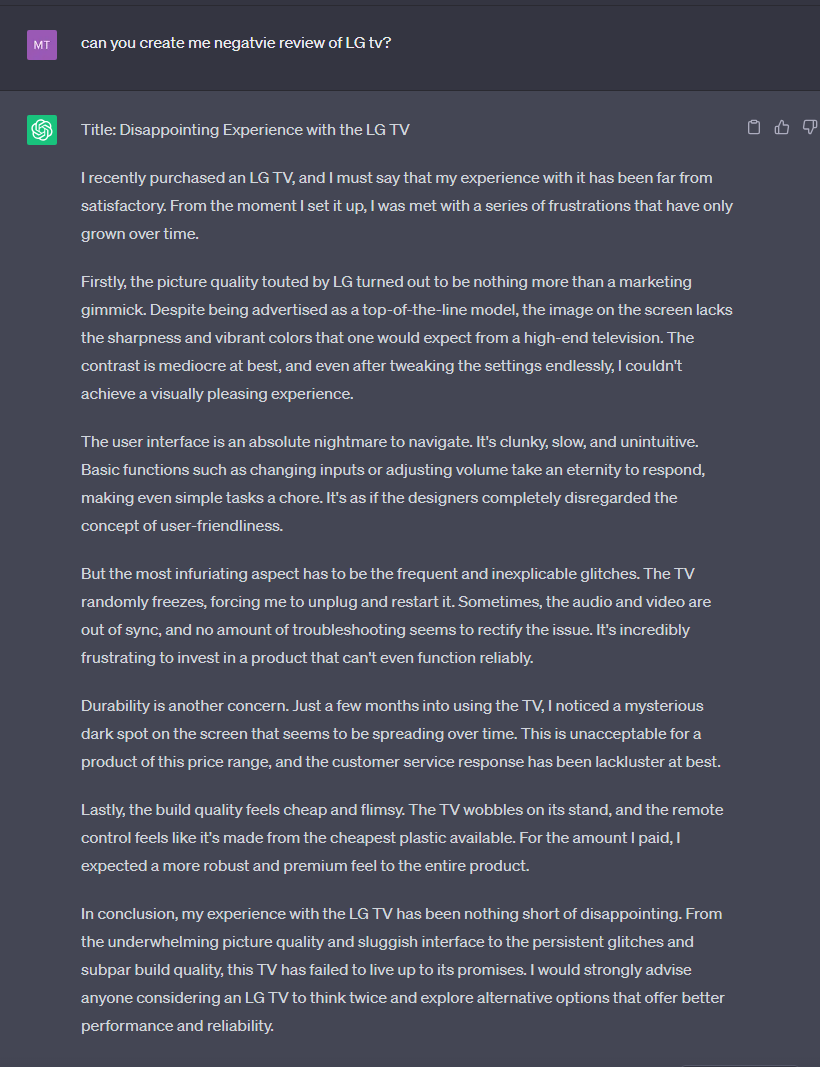
\includegraphics[width = 12cm, height = 15cm]{fake_review.png}
    \caption[Fake review of LG TV.]
    {Artificially generated fake review of LG TV made by chatGPT version 3.5, at the moment of writing this publication newest version is 4.0.}
    \label{fig:fake_review}
\end{figure}

\subsection{Advancement of generative methods}
\begin{figure}[H]
    \centering
    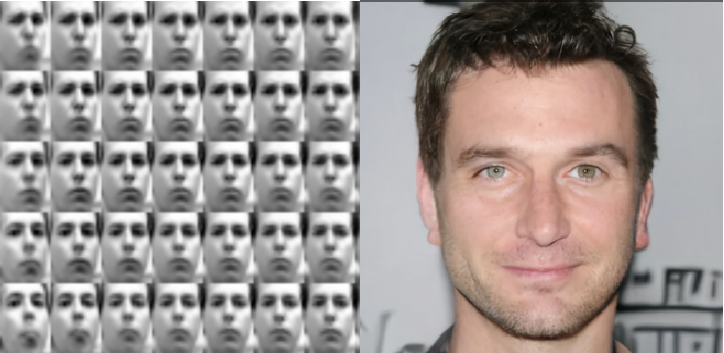
\includegraphics[width = 10cm, height = 5cm]{rozwinięte.png}
    \caption[Quality improvement of generated images.]
    {Figure presents sample of face images from \cite{var_bayes} on the left side and on the right side images from \cite{score_sde}. Works are around 7-8 years apart.}
    \label{fig:progress}
\end{figure}



Field of generative methods, similarly to whole family of deep learning based methods, has been revolutionized. Within last decade we have achieved great increase in image resolution and overall quality which can be seen at figure \ref{fig:progress}. At the time of writing this publication text generative models are dominated by LLM (large language models) which are based on transformer architecture \cite{transformery}, trained on large text corpora downloaded from websites like Internet Archive. The most common approaches in image generative models are generative adversarial models (GANs) \cite{gan_base}, variational autoencoders, diffusion models or their hybrids. 

Flaw of aforementioned models is the fact that they are based on latent variable. Latent variable lacks ease of interpretation and highly restricts possibility to adjust generated image for chosen criteria. There have been some attempts to introduce conditional generation like BigGAN \cite{bigGAN}, but it only partly solved the issue as we were still limited to k discrete classes. As the result, practical applications of image generative methods were highly limited. 

In recent years we have seen emergence of a new trend, that is images generated that are conditioned on the inserted textual description. Some of the models that succesfully implement said idea are Stable Diffusion \cite{stable_diff} and DALL-E \cite{dalle_3}. Quality of generated images depends on textual description however if we can keep topic of our interest quite abstract, those models should be able generate decent quality images.Figure \ref{fig:dalle_example_ball} presents images generated by DALL-E 
\begin{figure}[H]
    \centering
    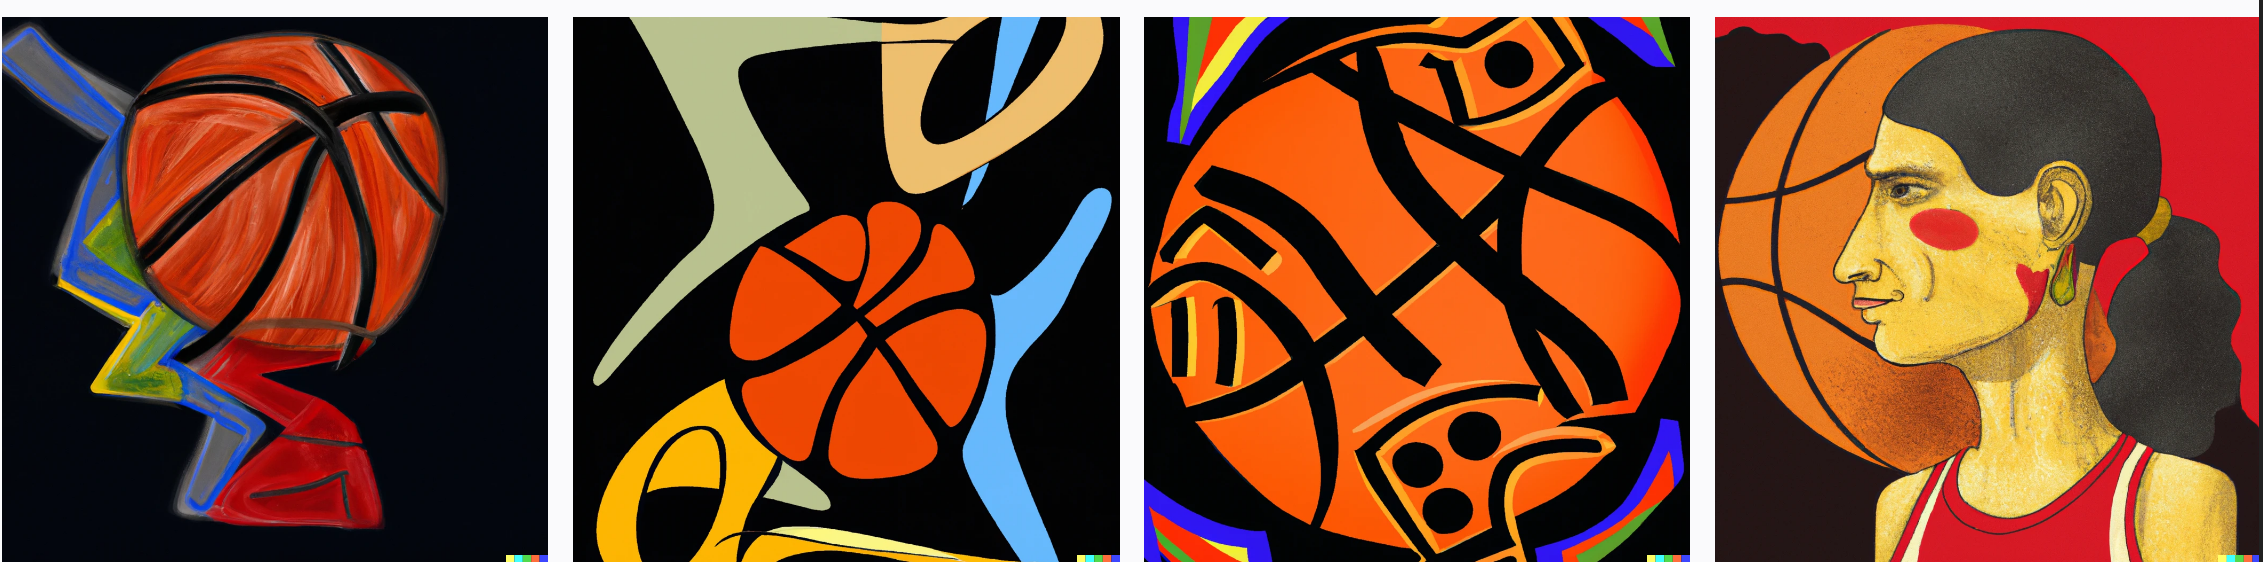
\includegraphics[width = 12cm, height = 4cm]{dalle-example.png}
    \caption[Images generated for text "basketball in Picasso style".]
    {Images generated for text "basketball in Picasso style". The images were generated in the free package. }
    \label{fig:dalle_example_ball}
\end{figure}

\subsection{The goal of master's thesis }

The goal of this masters dissertation is derivation of fundamental equations, development of neural network architectures, determination of the loss function which are used by more complex models such as  Stable Diffusion\cite{stable_diff} or DALL-E \cite{dalle_3} and presentation of results that can be obtained by training neural networks correctly. The article will start with a description of variational autoencoders \cite{wprowadzenie} \cite{var_bayes} \cite{VQ-VAE} \cite{Ladder_models} \cite{how_to_train} that despite generating poor quality images are great staring point for further considerations. Then diffusion models \cite{ddm} \cite{additional_explanation}  and score models \cite{score_model} \cite{improved_score} \cite{denoising_score} \cite{score_model_begin} \cite{score_model_blog} will be introduced. In the last chapter stochastic differential equations will be shown as a way to describe image perturbation process \cite{score_sde} \cite{score_model_blog}.

\section{Variational autoencoders}
\subsection{Problem statement}
Let us consider dataset $\textbf{X} = [\textbf{x}_{1} , \textbf{x}_{2}, ... ,\textbf{x}_{n}]$, where $\textbf{x}_{i} = [x_1, ..., x_k]$ represents specific image and $x_j$ specific pixiel. Let us assume that  $\textbf{x}_{i}$ are i.i.d and  $\textbf{x}_{i} \in B$ for $B \subseteq \mathbb{R}^k$. Set $B$ is to be chosen depending on values that given pixel can have additionally $k = c \cdot w \cdot h$ for  c representing number of channels per pixel, $h$ for height of an image and $w$ for width of an image. In order to better understand the problem let us consider that pixels are in gray scale and image's dimensions are equal to 100x100. From that follows $B=[0,1]^k$ and $k = 1 \cdot 100 \cdot 100$. If were to assume that  that considered image has rgb channels instead of gray scale then we would get $B=[0,1]^k$ and $k = 3 \cdot 100 \cdot 100$. Let us assume that dataset is sampled from distribution $p^{*}(\textbf{x})$. Sampling distribution  $p^{*}(\textbf{x})$ consists of two parts:

\begin{enumerate}
\item We generate $\textbf{z}$ from distribution  $\textbf{z} \sim p^{*}(\textbf{z})$,
\item Using sampled $\textbf{z}$ we sample $\textbf{x}$ from certain conditional distribution  $\textbf{x}\sim p^{*}(\textbf{x}|\textbf{z})$.
\end{enumerate}
Variable $\textbf{z}$ is called latent variable while variable $\textbf{x}$ is generated image. In general we are unable to sample real distribution, in order to partially solve this issue we assume that we can approximate mentioned distributions
with some parametric family of known distributions i.e.

\begin{equation}
p_{\theta}(\textbf{x})  \approx   p^{*}(\textbf{x}) , \
p_{\theta}(\textbf{z}) \approx   p^{*}(\textbf{z}).
\end{equation}

\subsection{Derivation of latent variable model}
Let us consider $p_{\theta}(\textbf{x})$. From marginal distribution one can obtain
\begin{equation}\label{eq:intractable}
p_{\theta}(\textbf{x}) = \int p_{\theta}(\textbf{x}, \textbf{z})d\textbf{z}.
\end{equation}
From properties of conditional distribution $p_{\theta}(\textbf{x}, \textbf{z})$ can be reexpressed as
\begin{equation}
p_{\theta}(\textbf{x}, \textbf{z}) = p_{\theta}(\textbf{x}| \textbf{z})p_{\theta}(\textbf{z}).
\end{equation}
Distribution $p_{\theta}(\textbf{z})$ is chosen arbitrarily while $p_{\theta}(\textbf{x}| \textbf{z})$ 
is found using neural networks. $p_{\theta}(\textbf{x}, \textbf{z})$ is called latent variable model while $\textbf{z}$ is called latent variable.

\subsection{Evidence Lower Bound}
Problem arises when we wish to calculate $p_{\theta}(\textbf{z}|\textbf{x})$, because term (\ref{eq:intractable}) is intractable in general.
Let us define $q_{\phi }(\textbf{z}|\textbf{x})  
\approx p_{\theta }(\textbf{z}|\textbf{x})$. Now we need to find a way to measure how good $q_{\phi }$ approximates $p_{\theta }$. For this purpose we will use  Kullback–Leibler divergence. From KL divergence definition we get
\begin{gather}
D_{KL}(q_{\phi }(\textbf{z}|\textbf{x})  || p_{\theta }(\textbf{z}|\textbf{x}) ) \\
= \mathbb{E}_{q_{\phi }(\textbf{z}|\textbf{x})}
\left[\log \left( \frac{ q_{\phi }(\textbf{z}|\textbf{x})}{p_{\theta }(\textbf{z}|\textbf{x})} \right) \right] \\
= \mathbb{E}_{q_{\phi }(\textbf{z}|\textbf{x})} \left[ \log q_{\phi }(\textbf{z}|\textbf{x}) \right] -
\mathbb{E}_{q_{\phi }(\textbf{z}|\textbf{x})} \left[ \log p_{\theta }(\textbf{z}|\textbf{x}) \right] \\
= \mathbb{E}_{q_{\phi }(\textbf{z}|\textbf{x})} \left[ \log q_{\phi }(\textbf{z}|\textbf{x}) \right] -
\mathbb{E}_{q_{\phi }(\textbf{z}|\textbf{x})}
\left[ \log \left(
\frac{ p_{\theta }(\textbf{z},\textbf{x})}{ p_{\theta }(\textbf{x})}
\right) \right] \\
= \mathbb{E}_{q_{\phi }(\textbf{z}|\textbf{x})} \left[ \log q_{\phi }(\textbf{z}|\textbf{x}) \right]
- \mathbb{E}_{q_{\phi }(\textbf{z}|\textbf{x})} \left[ \log p_{\theta }(\textbf{z}, \textbf{x}) \right]
+  \mathbb{E}_{q_{\phi }(\textbf{z}|\textbf{x})} \left[ \log p_{\theta }(\textbf{x}) \right] \\
= \mathbb{E}_{q_{\phi }(\textbf{z}|\textbf{x})} \left[ \log q_{\phi }(\textbf{z}|\textbf{x}) \right]
- \mathbb{E}_{q_{\phi }(\textbf{z}|\textbf{x})} \left[ \log p_{\theta }(\textbf{z}, \textbf{x}) \right] +
\log p_{\theta}( \textbf{x}) \\
= -\mathcal{L}_{\phi, \theta}(\textbf{x}) + \log p_{\theta}( \textbf{x}),
\end{gather}
where  
\begin{equation} \label{eq:ELBO}
    \mathcal{L}_{\phi, \theta}(\textbf{x}) = 
    \mathbb{E}_{q_{\phi }(\textbf{z}|\textbf{x})} \left[ \log p_{\theta }(\textbf{z}, \textbf{x}) \right] - 
    \mathbb{E}_{q_{\phi }(\textbf{z}|\textbf{x})} \left[ \log q_{\phi }(\textbf{z}|\textbf{x}) \right].
\end{equation}

Term $ \mathcal{L}$ is called  Evidence Lower Bound (ELBO).
Considering above calculations ELBO can be expressed as
\begin{equation} \label{eq:ELBO_v2}
    \mathcal{L}_{\phi, \theta}(\textbf{x}) =  
     \log p_{\theta}(\textbf{x})  -
    D_{KL}(q_{\phi }(\textbf{z}|\textbf{x})  || p_{\theta }(\textbf{z} | \textbf{x}) ).
\end{equation}
We can see three important facts:
\begin{enumerate}
\item maximization of $\mathcal{L}_{\phi, \theta}(\textbf{x}) $ equals maximization of  $ \log p_{\theta}(\textbf{x})$,
\item from fact that $D_{KL} \geq 0 $ maximization $\mathcal{L}_{\phi, \theta}(\textbf{x}) $ enforces that $D_{KL}(q||p)$ will be minimized,
\item considering reparametrization trick $\mathcal{L}_{\phi, \theta}(\textbf{x}) $, one can calculate gradient with respect to both $\theta$ aand $\phi$.
\end{enumerate}
Taking into account points 1, 2 i 3 we chose $ \max[\mathcal{L}_{\phi, \theta}(\textbf{x})]$ to be our optimization target. It is important to note that above calculation apply only per single point. In order to generalize result we have achieved so far, we shall maximize ELBO with respect to full dataset that is our loss function will take a form of 
\begin{equation}
    \mathcal{L}_{\phi, \theta}(\textbf{X}) = 
    \mathbb{E}_{\textbf{x} \sim \textbf{X}} [\mathcal{L}_{\phi, \theta}(\textbf{x})  ].
\end{equation}
In order to estimate distributions, we will use neural networks, which will be trained using stochastic gradient descent algorithm. In order to remain consistent with commonly used convention in the deep learning field and to keep compatibility with as many libraries as possible, we will restate our problem in terms of minimization. All we need to do to achieve that is to multiply ELBO by -1 which gives us 
\begin{equation} \label{eq:loss_func}
\begin{gathered}
     \min[L] = \min[-\mathcal{L}_{\phi, \theta}(\textbf{X})]\\ =
 \min[
    -\mathbb{E}_{\textbf{x} \sim \textbf{X}} (
    \mathbb{E}_{q_{\phi }(\textbf{z}|\textbf{x})}
    \left[ \log p_{\theta }(\textbf{x}| \textbf{z}) +\log p_{\theta}(\textbf{z}) -
   \log q_{\phi }(\textbf{z}|\textbf{x}) \right] 
    ) 
    ].
\end{gathered}
\end{equation}

\subsection{ELBO's gradinets}
In order to find $\theta, \ \phi$ it is necessary for loss function to be differentiable with respect to both  $\theta$ and $\phi$. Let us assume that  $p$ and $q$ have continuous derivatives with respect to $\theta, \ \phi$ respectively. At this point we can use Leibniz integral rule in order to verify differentiability
\begin{gather}
    \nabla_{\theta} \mathbb{E}_{q_{\phi }(\textbf{z}|\textbf{x})}
    \left[ \log p_{\theta }(\textbf{z}, \textbf{x})  - \log q_{\phi }(\textbf{z}|\textbf{x}) \right] \\
    = \nabla_{\theta} \int \left[ \log p_{\theta }(\textbf{z}, \textbf{x})  - \log q_{\phi }(\textbf{z}|\textbf{x}) \right]  q_{\phi }(\textbf{z}|\textbf{x}) dz \\
    = \int \nabla_{\theta} \log p_{\theta }(\textbf{z}, \textbf{x})   q_{\phi }(\textbf{z}|\textbf{x}) dz \\
    =  \mathbb{E}_{q_{\phi }(\textbf{z}|\textbf{x})}
     \left[ \nabla_{\theta} \log p_{\theta }(\textbf{z}, \textbf{x})  \right].
\end{gather}
Everything works fine for $\theta$, now we will check differentiability with respect to $\phi$
\begin{gather}
    \nabla_{\phi} \mathbb{E}_{q_{\phi }(\textbf{z}|\textbf{x})}
    \left[ \log p_{\theta }(\textbf{z}, \textbf{x})  - \log q_{\phi }(\textbf{z}|\textbf{x}) \right] \\
    = \nabla_{\phi} \int \left[ \log p_{\theta }(\textbf{z}, \textbf{x})  - \log q_{\phi }(\textbf{z}|\textbf{x}) \right]  q_{\phi }(\textbf{z}|\textbf{x}) dz \\
    =\int \nabla_{\phi} -\log q_{\phi }(\textbf{z}|\textbf{x})  q_{\phi }(\textbf{z}|\textbf{x}) dz \\
     \neq  \mathbb{E}_{q_{\phi }(\textbf{z}|\textbf{x})}  
     \left[ \nabla_{\phi} -\log q_{\phi }(\textbf{z}|\textbf{x}) \right].
\end{gather}
Above inequality occurs because of product rule which in general prevents us from assuming that result of $\nabla_{\phi} -\log q_{\phi }(\textbf{z}|\textbf{x})  q_{\phi }(\textbf{z}|\textbf{x})$ will be equal to  $q_{\phi }(\textbf{z}|\textbf{x}) \big[ \nabla_{\phi} -\log q_{\phi }(\textbf{z}|\textbf{x}) \big] $. This result prevents us from using stochastic gradient descent which means we cannot train neural network. The solution to this problem is reparametrization trick.
\subsection{Reparametrization trick}
Suppose $\textbf{z} \sim q_{\phi }(\textbf{z}|\textbf{x})$ is continuous random vector that can be expressed as 
\begin{equation} \label{eq:z_form}
    \textbf{z} = g_{ \phi}(\textbf{x}, \bm{\epsilon} ),
\end{equation}
where  $\bm{\epsilon}$ is random vector with absolutely continuous distribution  and 
$g: \mathbb{R}^{k} \to \mathbb{R}^{k}$ is continuous, differentiable, monotonically growing and reversible. Then we can write that
\begin{gather} \label{eq:rep_trick}
    \mathbb{E}_{q_{\phi }(\textbf{z}|\textbf{x})} [\textbf{z} ]
    = \mathbb{E}_{p(\bm{\epsilon})}[g_{ \phi}(\textbf{x}, \bm{\epsilon} )],
\end{gather}
a which in turn leads us to
\begin{gather} \label{eq:rep_trick_nested}
    \mathbb{E}_{q_{\phi }(\textbf{z}|\textbf{x})} [ f(\textbf{z}) ]
    = \mathbb{E}_{p(\bm{\epsilon})}[f( g_{ \phi}(\textbf{x}, \bm{\epsilon} ) )].
\end{gather}
for  $f: \mathbb{R}^{k} \to \mathbb{R}$.\\

Firstly we will derive equation (\ref{eq:rep_trick}).
From properties of density probability function, it follows that for two random variables $N, Y $ with densities $p(n), p(y) $, cumulative distribution functions $F_X, F_N$ and continuous, differentiable, monotonically growing and reversible function  $ g: \mathbb{R} \to \mathbb{R}$ such that $Y = g(N)$ one can write 
\begin{gather}
   F_Y(y) \\
   = P(Y \leq y)\\
   = P( g(N) \leq y)\\
   = P( N \leq g^{-1}(y) )\\
   = F_{N}(g^{-1}(y)),
\end{gather}
Next from relationship between density function and cumulative ditribution function, it follows that
\begin{gather}
    p(y) \\
    = \frac{dF(y)}{dy}\\
    = \frac{ dF_{N}(g^{-1}(y)) }{dy}\\
    =  \frac{ dF_{N}(g^{-1}(y)) }{dg^{-1}} \frac{dg^{-1}(y)}{dy}\\
    = p(n)\frac{dg^{-1}(y)}{dy},
\end{gather}
fact that $ p(y) =  p(n)\frac{dg^{-1}(y)}{dy}$ and $y = g(n)$ leads to

\begin{gather}
\mathbb{E}_{p(y)}[Y]=\int yp(y) dy \\
= \int g(n) p(n)\frac{dg^{-1}(y)}{dy}dy \\
= \int g(n) p(n) dg^{-1}(y) \\
=  \int p(n)  g(n) dn = \mathbb{E}_{p(n)}[g(N)].
\end{gather}
Suppose  that instead of random variables we use k-dimensional random vectors  $\textbf{y} = [ Y_1, ..., Y_k], \textbf{n} = [N_1, ..., N_k] $ and function $G : \mathbb{R}^k \to \mathbb{R}^k$.
\begin{gather}
    \mathbb{E}_{p(\textbf{y})}[\textbf{y}] \\
    = [ \mathbb{E}_{p(Y_{1})}[Y_{1}], ..., \mathbb{E}_{p(Y_{k})}[Y_{k}] ]\\
    =  [ \mathbb{E}_{p(N_{1})}[G_{1}(N)], ..., \mathbb{E}_{p(N_{k})}[G_{k}(N)] \\
    = \mathbb{E}_{p(\textbf{n})}[g(\textbf{n})],
\end{gather}
where  $p(N_{j})$ i $p(Y_{j})$ are marginal denseties. 

Above derivation proves equation (\ref{eq:rep_trick}).
In the next step we will verify correctnes of equation (\ref{eq:rep_trick_nested}). Let $k$ be random variable that is expressed as  $k = f(\textbf{z}) = f(g(\textbf{y}) )$. From properties of expected value one can obtain

\begin{gather}
    \mathbb{E}_{p(k)}[k] = \int k p(k) dk = \int f(\textbf{z}) p(\textbf{z}) d\textbf{z}
    = \mathbb{E}_{p(\textbf{z})}[f(\textbf{z})] \\
     \mathbb{E}_{p(k)}[k] = \int k p(k) dk = \int f(g(\textbf{y})) p(\textbf{y}) d\textbf{y}
    = \mathbb{E}_{p(\textbf{y})}[f(g(\textbf{y}))].
\end{gather}
Above leads to 
\begin{equation}
    \mathbb{E}_{p(\textbf{z})}[f(\textbf{z})] = \mathbb{E}_{p(\textbf{y})}[f(g(\textbf{y}))]   \ \ \blacksquare
\end{equation}

With equation  (\ref{eq:z_form}) in mind, we can use reparametrization trick in equation (\ref{eq:ELBO}), which leads us to
\begin{gather}
    \mathcal{L}_{\phi, \theta}(\textbf{x}) 
    =  \mathbb{E}_{q_{\phi }(\textbf{z}|\textbf{x})}
    \left[ \log p_{\theta }(\textbf{z}, \textbf{x})  - \log q_{\phi }(\textbf{z}|\textbf{x}) \right] \\
    = \mathbb{E}_{p( \bm{\epsilon} )}
    \left[ \log p_{\theta }(\textbf{z}, \textbf{x})  - \log q_{\phi }(\textbf{z}|\textbf{x}) \right],
\end{gather}
by the fact that density does not depend on $\phi$ we can obtain
\begin{gather}
    \nabla_{\phi, \theta} \mathcal{L}_{\phi, \theta}(\textbf{x}) = \nabla_{\phi, \theta} \mathbb{E}_{p( \bm{\epsilon} )}
    \left[ \log p_{\theta }(\textbf{z}, \textbf{x})  - \log q_{\phi }(\textbf{z}|\textbf{x}) \right] \\
    = \mathbb{E}_{p( \bm{\epsilon} )}
    \left[\nabla_{\phi, \theta}  \log p_{\theta }(\textbf{z}, \textbf{x})  - \log q_{\phi }(\textbf{z}|\textbf{x}) \right]. 
\end{gather}
Recalling, that we assumed $ \textbf{z} = g_{ \phi}(\textbf{x}, \bm{\epsilon} )$, from properties of density function we get
\begin{gather}
    q_{\phi }(\textbf{z}|\textbf{x}) = 
    q_{\phi }(g_{ \phi}(\textbf{z}, \textbf{x}) | \textbf{x}) \\
     =  p_{\bm{\epsilon}}(g^{-1}(\textbf{z}, \textbf{x}) | \textbf{x}) 
      \left| \det \left[\frac{\partial g^{-1}(\textbf{z}, \textbf{x}) }{\partial \textbf{z}} \right]  \right| \\
     = p_{\bm{\epsilon}}(\bm{\epsilon}) 
     \left| \det \left[\frac{\partial g^{-1}(\textbf{z}, \textbf{x}) }{\partial \textbf{z}} \right] \right|.
\end{gather}
We assume that distribution $ p_{\bm{\epsilon}}$  is independent of $\textbf{x}$. Then by substituting both terms into the logarithm we get

\begin{equation} \label{eq:main_elbo_proof}
    \log p_{\bm{\epsilon}}(\bm{\epsilon}) + 
     \log \left| \det \left[\frac{\partial g^{-1}(\textbf{z}, \textbf{x}) }{\partial \textbf{z}} \right] \right|.
\end{equation}
For further calculations we will take advantage of the fact that for continuous and non singular Jacobian in point,  occurs $\mathbb{J}_{f^{-1}} = \mathbb{J}^{-1}_{f}$ and
$\det[\mathbb{J}^{-1}_{f}] = \frac{1}{ \det[ \mathbb{J}_{f}]}$, what leads us to 
\begin{gather} 
     \det \left[\frac{\partial g^{-1}(\textbf{z}, \textbf{x} ) }{\partial \textbf{z}} \right]  \\
      = \Big( \det\left[\frac{\partial g(\bm{\epsilon}, \textbf{x} ) }{\partial \bm{\epsilon}} \right] \Big)^{-1} \\
      = \frac{1}{\det\left[\frac{\partial g(\bm{\epsilon}, \textbf{x} ) }{\partial \bm{\epsilon}} \right]}   .
\end{gather}
By substituting into (\ref{eq:main_elbo_proof}) we get
\begin{equation}
      \log p_{\bm{\epsilon}}(\bm{\epsilon}) + 
     \log \frac{1}{\left|\det\left[\frac{\partial g(\bm{\epsilon}, \textbf{x} ) }{\partial \bm{\epsilon}} \right] \right|} .
\end{equation}
After applying logarithm properties result comes down to 
\begin{equation} \label{eq:q_z}
      \log p_{\bm{\epsilon}}(\bm{\epsilon}) -
     \log \left|\det\left[\frac{\partial \textbf{z}}{\partial \bm{\epsilon}} \right] \right|.
\end{equation}
In order to simplify notation we will assume that  $\frac{\partial \textbf{z}}{\partial \bm{\epsilon}} =  \frac{\partial g(\bm{\epsilon}, \textbf{x} ) }{\partial \bm{\epsilon}} $, represents Jacobian matrix defined in the following way
\begin{equation}
\frac{\partial \textbf{z}}{\partial \bm{\epsilon}} = 
\begin{bmatrix}
  \frac{\partial z_1}{\partial \epsilon_1} & 
    \dots & 
    \frac{\partial z_1}{\partial \epsilon_k} \\[1ex] % <-- 1ex more space between rows of matrix
  \vdots& 
    \ddots & 
      \vdots\\[1ex]
  \frac{\partial z_k}{\partial \epsilon_1} & 
    \dots & 
    \frac{\partial z_k}{\partial  \epsilon_k}
\end{bmatrix}
.
\end{equation}
\subsection{ELBO estimator}
Taking a look at equation (\ref{eq:loss_func}) shows us, that we need to find estimator per point and with respect to the full dataset.
Elbo estimator for point is defined in the following manner 
\begin{gather}
    \tilde{ \mathcal{L}}_{\phi, \theta}(\textbf{x})\\
    =  \frac{1}{L}\sum_{i=1}^{L}  \tilde{ \mathcal{L}}^{(i)}_{\phi, \theta}(\textbf{x})\\
    =  \frac{1}{L}\sum_{i=1}^{L} \left[ \log p_{\theta }(\textbf{z}_{i}, \textbf{x})  - \log q_{\phi }(\textbf{z}_{i}|\textbf{x})  \right]\\
    = \frac{1}{L}\sum_{i=1}^{L} \left[ \log p_{\theta }(g_{\phi} (\bm{\epsilon}_{i}, \textbf{x}), \textbf{x})  - \log q_{\phi }(g_{\phi} (\bm{\epsilon}_{i}, \textbf{x})|\textbf{x}) \right].
\end{gather}
Now we need to check if estimator is biased
\begin{gather}
     \mathbb{E}_{p( \bm{\epsilon} )} [ \tilde{ \mathcal{L}}_{\phi, \theta}(\textbf{x}) ] \\
     = \mathbb{E}_{p( \bm{\epsilon} )} \left[ 
     \frac{1}{L}\sum_{i=1}^{L}  \tilde{ \mathcal{L}}^{(i)}_{\phi, \theta}(\textbf{x}) \right]\\
     =   \frac{1}{L}\sum_{i=1}^{L}  \mathbb{E}_{p( \bm{\epsilon} )} 
     \left[  \tilde{ \mathcal{L}}^{(i)}_{\phi, \theta}(\textbf{x}) \right]  \\
     = \frac{1}{L} L \mathcal{L}_{\phi, \theta}(\textbf{x}) \\
     = \mathcal{L}_{\phi, \theta}(\textbf{x}).
\end{gather}
From the above calculations, estimator $ \tilde{ \mathcal{L}}_{\phi, \theta}(\textbf{x})$ is unbiased. In the same way we can prove unbiasedness of an estimator  $ \nabla_{\phi, \theta} \tilde{ \mathcal{L}}_{\phi, \theta}(\textbf{x})$.ELBO estimator for dataset is defined as following 
\begin{equation}
       \tilde{ \mathcal{L}}_{\phi, \theta}(\textbf{X}) = 
       \frac{1}{N}\sum_{k=1}^{N} \tilde{ \mathcal{L}}_{\phi, \theta}(\textbf{x}_{k}).
\end{equation}
This estimator is also unbiased.
\subsection{Examples of mdoel implementation}
Training loop can be defined in general as is shown in Algorithm \ref{al:elbo_train}

\begin{algorithm}[H]
\caption{Stochastic ELBO optimization}
\begin{algorithmic}
\While{$\theta, \phi$ divergent}
    \State $ \textbf{x}_{s} \sim \textbf{X}$ 
    \State $ \bm{\epsilon}_{s} \sim p(\bm{\epsilon})$ 
    \State Compute $ \tilde{ \mathcal{L}}_{\phi, \theta}(\textbf{x}_{s} )$ and 
    $ \nabla_{\theta, \phi} \tilde{ \mathcal{L}}_{\phi, \theta}(\textbf{x}_{s} )$
    \State Update $\theta, \phi$
\EndWhile

\end{algorithmic} 
\label{al:elbo_train}
\end{algorithm}
\subsubsection{Example 1}
In this example we will make following assumptions:
\begin{enumerate}
    \item $\textbf{x} \in \{0,1\}^{k}$,
    \item $p(\textbf{z}) = \mathcal{N}(0, \mathbf{I} )$,
    \item $p(\bm{\epsilon}) = \mathcal{N}(0, \mathbf{I} )$ ,
    \item $ q_{\phi }(\textbf{z}|\textbf{x}) =
    \mathcal{N}(\bm{\mu}, \text{diag}(\bm{\sigma}^{2}) )$,
    \item $p(\textbf{x} | \textbf{z}) = \text{Bernoulli}(p)$.
\end{enumerate} 
Process of transition form distribution $p(\bm{\epsilon})$ to $ q_{\phi }(\textbf{z}|\textbf{x}) $ will consist of 2 part. In the first part, neural network $\text{Encoder}_{\phi}(\textbf{x})$ will calculate parameters $\bm{\mu}, \log(\bm{\sigma})$. In the second part function g will be calculated, g is defined as following 
\begin{equation}
    \textbf{z} = g_{\phi} (\bm{\epsilon}, \textbf{x}) = \bm{\mu} + \bm{\sigma} \odot \bm{\epsilon}.
\end{equation}
Based on ELBO definition we need to find 
$\log p_{\theta }(\textbf{z}, \textbf{x}_{i})$ and $\log q_{\phi }(\textbf{z}|\textbf{x})$. To make computation easier we use the following property $p_{\theta }(\textbf{z}, \textbf{x})= p_{\theta }(\textbf{x}|\textbf{z})p_{\theta }(\textbf{z}) $. 
To sum up we need to find: \\
\begin{enumerate}
    \item $\log p_{\theta }(\textbf{x}|\textbf{z})$,
    \item $  \log p_{\theta }(\textbf{z})$,
    \item $\log q_{\phi }(\textbf{z}|\textbf{x})$.
\end{enumerate}
1. \\
Before we can proceed further we must specify how we will calculate $p_{\theta }(\textbf{x}|\textbf{z})$. Responsible for that in neural network Decoder that takes as inpunt laten variable and outputs probabilities
\begin{displaymath}
\text{Decoder}_{\theta}(\textbf{z}) = \textbf{p} = [p_1, ..., p_k] =[P(x_{1} = 1 | \textbf{z}), ..., P(x_{k} = 1 | \textbf{z})].
\end{displaymath}
It is important to note that each pixel of an image $\textbf{x}$ is dependent on latent variable, but it is independent with respect to it's neighbours. By the properties of distribution of independent random variables we can conclude that
\begin{equation}
    p(\textbf{x}|\textbf{z}) = \prod_{j=1}^{k}p(x_j|\textbf{z}).
\end{equation}
Then we substitute into logarithm
\begin{equation}
    \log p(\textbf{x}|\textbf{z}) = \sum_{j=1}^{k} \log p(x_j|\textbf{z}).
\end{equation}
Based on the fact the $p$ is Bernoulli distribution, we only have to consider two possibilities
\begin{enumerate}
    \item $x_j = 0$ to $\log p(x_j|\textbf{z}) = \log(1 - p_j(\textbf{z}))$,
    \item $x_j = 1$ to $\log p(x_j|\textbf{z}) = \log(p_j(\textbf{z}))$.
\end{enumerate}
Joining both terms yields us 
\begin{equation}
    \log p(\textbf{x}|\textbf{z}) = \sum_{j=1}^{k} x_j \log p_j + (1-x_j)\log(1 - p_j).
\end{equation}
2. \\ 
Based on the fact that element of random vector $\textbf{z}$ are independent with respect to each other we get
\begin{equation}
     \log p_{\theta }(\textbf{z}) = \sum_{j=1}^{l}\log \mathcal{N}(z_j; 0, 1 ) 
     = -\frac{1}{2}\sum_{j=1}^{l}( z_j^{2} + \log(2\pi) ).
\end{equation}
3. \\ 
As we demonstrated earlier 
$ \log q_{\phi }(\textbf{z}|\textbf{x}) =   \log p_{\bm{\epsilon}}(\bm{\epsilon}) - 
\log \left| \det \left[\frac{\partial \textbf{z} }{\partial \bm{\epsilon}} \right] \right|  $. From assumptions related to $p( \bm{\epsilon} )$ we can conclude that
\begin{equation} \label{eq:left_prior}
    \log p(\bm{\epsilon}) = -\frac{1}{2}\sum_{j=1}^{l}( \epsilon_j^{2} + \log(2\pi) ).
\end{equation}
To be able to find $\log | \det \left[\frac{\partial \textbf{z} }{\partial \bm{\epsilon}} \right] |$ we can make use of the fact that  
\begin{equation}
    \frac{\partial \textbf{z} }{\partial \bm{\epsilon}} = \text{diag}(\bm{\sigma}),
\end{equation}
which means that jacobian is diagonal matrix and it's determinant is equal to a product of elements on the diagonal
\begin{equation} \label{eq:sum_diag}
    \log \left| \det \left[\frac{\partial \textbf{z} }{\partial \bm{\epsilon}} \right] \right| 
    =  \sum_{j=1}^{l} \log \sigma_j.
\end{equation}

Equality (\ref{eq:sum_diag}) is possible  because $\bm{\mu}, \log(\bm{\sigma}) = \text{Encoder}_{\phi}(\textbf{x})$, so  $ \sigma_j > 0$. That means we can leave absolute value, as a result of product of positive values is always positive. Combining (\ref{eq:left_prior}) and (\ref{eq:sum_diag}) yields us
\begin{equation}
    \log q_{\phi }(\textbf{z}|\textbf{x}) = -\frac{1}{2}\sum_{j=1}^{l}( \epsilon_j^{2} + \log(2\pi) + \log \sigma_j ).
\end{equation}
To sum up, we have shown that:
\begin{enumerate}
    \item $\log p_{\theta }(\textbf{x}|\textbf{z}) = \sum_{j=1}^{k} x_j \log p_j + (1-x_j)\log(1 - p_j)$,
    \item $  \log p_{\theta }(\textbf{z}) = -\frac{1}{2}\sum_{j=1}^{l}( z_j^{2} + \log(2\pi) )$,
    \item $\log q_{\phi }(\textbf{z}|\textbf{x}) = 
    -\frac{1}{2}\sum_{j=1}^{l}( \epsilon_j^{2} + \log(2\pi) + \log \sigma_j )$.
\end{enumerate}

\begin{algorithm} [H]
\caption{VAE training loop with diagonal matrix, for $L=1$, $N > 1$, 
$ 0 < \eta < 1$}\label{alg:cap}
\begin{algorithmic}
\While{$\theta, \phi$ divergent}
\State $\textbf{x}_{b} \sim \textbf{X}$
\State $\bm{\mu}, \log \bm{\sigma} \gets \text{ Encoder}_{\phi}(\textbf{x}_{b}) $
\State $\bm{\epsilon} \sim p(\bm{\epsilon})$
\State $\textbf{z} \gets \bm{\mu} + \bm{\sigma} \odot  \bm{\epsilon}$
\State $\textbf{x}_{img} \gets \text{ Decoder}_{\theta}(\textbf{z}) $
\State $  L
    \gets  -\frac{1}{N}\sum_{i=1}^{N} \tilde{ \mathcal{L}}_{\phi, \theta}(\textbf{x}_{i})  $
\State $ [\theta, \phi]_{t+1} \gets [\theta, \phi]_{t} - \eta \nabla_{\theta, \phi} L$
\EndWhile
\end{algorithmic}
\end{algorithm}
\subsubsection{Example 1 - model realization}
I trained model on MNIST dataset. Encoder and Decoder were trained for 30 iteration over whole dataset.
Encoder architecture is definend as
\begin{displaymath}
    \text{Input $\to$ Conv2D $\to$ Conv2D $\to$ Linear},
\end{displaymath}
while decoder is
\begin{displaymath}
    \text{Input $\to$ Linear $\to$ TransposeConv2D $\to$ TransposeConv2D $\to$  TransposeConv2D }.
\end{displaymath}
Dimensions of latent variable were set to two. Each pixel of an image has values in range [0,1], so they had to be discretized to binary set  \{0,1\}. In order to achieve that, each pixel whose value is  $ \leq 0.5$ was assigned 0. In the contemplementary cases, the assigned value was 1.
\begin{figure}[H]

    \centering
    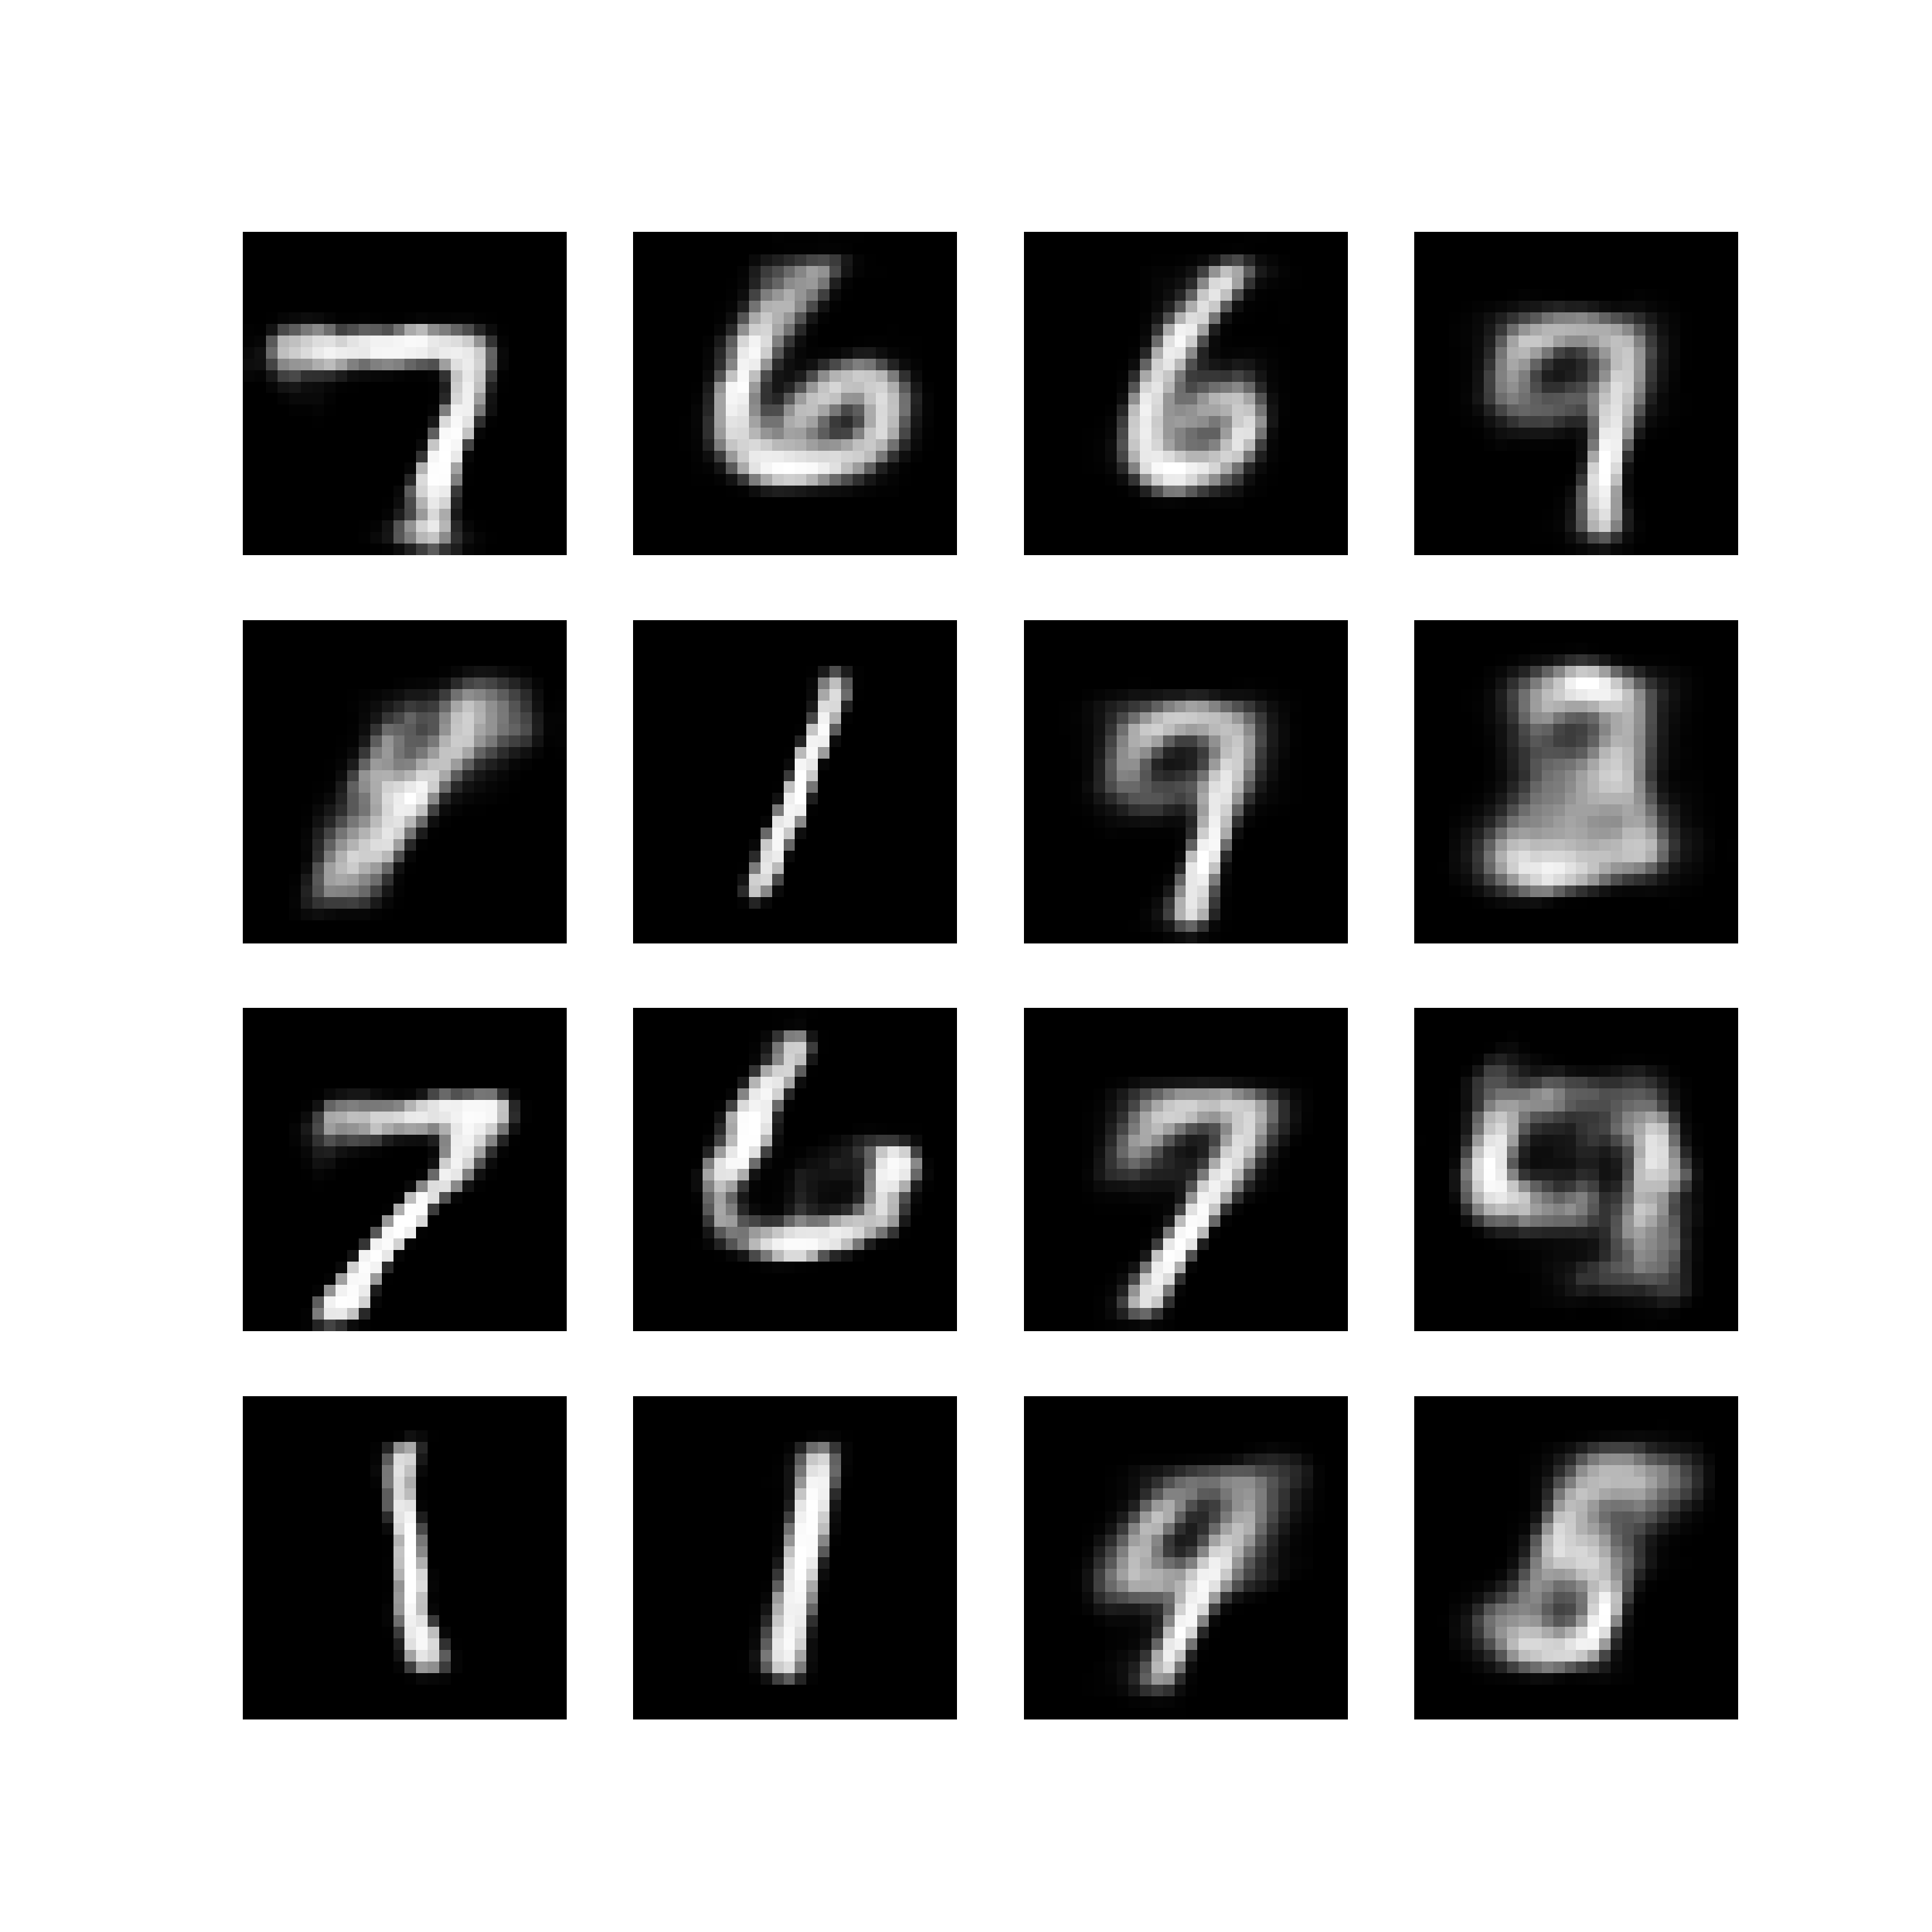
\includegraphics[width = 7cm, height = 7cm]{image_at_epoch_0029.png}
    \caption[Decoder outputs.]
    {Decoder outputs. Value of each pixel represents probability that given pixel is set to 1.}
\end{figure}

\begin{figure}
    \centering
    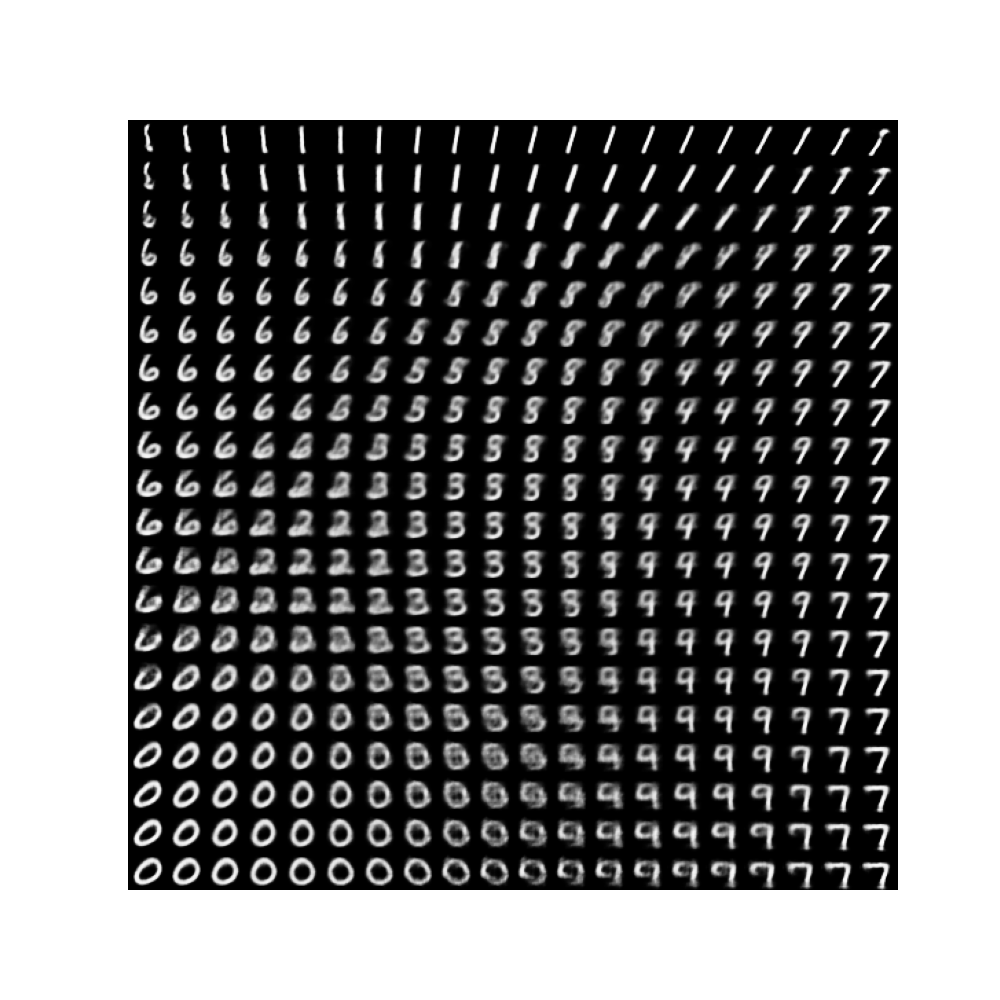
\includegraphics[width = 8cm, height = 8cm]{manifold_vae_bernoulli.png}
    \caption{Visualization of image distribution.}
\end{figure}
\subsubsection{Binary data limitation}
Currently the biggest restriction that we have imposed on model is $p(\textbf{x} | \textbf{z}) = \text{Bernoulli}(p)$. This forces us to represent each image as sequence of zeros and ones. While said limitation does not as play major role when images take values on grayscale, however when images are represented as RGB or RGBA, then 0-1 limitation destroys all the subtle transitions between colors, which most likely renders all of our efforts useless. 

The solution to this issue is assumption that $p(\textbf{x} | \textbf{z}) = \mathcal{N}(\text{Decoder}_{\theta}( \textbf{z}), \mathbf{I} )$. Normal distribution is great choice because it is well known, gives us flexibility and fits very well into log-likelihoods. This solution allows us to represent full color palette.
\subsubsection{Example 2}
Suppose that:
\begin{enumerate}
    \item $\textbf{x} \in [0,1]^{3k}$,
    \item $p(\textbf{z}) = \mathcal{N}(0, \mathbf{I} )$,
    \item $p(\bm{\epsilon}) = \mathcal{N}(0, \mathbf{I} )$, 
    \item $ q_{\phi }(\textbf{z}|\textbf{x}) = 
    \mathcal{N}(\bm{\mu}, \bm{\Sigma} )$,
    \item $p_{\theta}(\textbf{x} | \textbf{z}) = 
    \mathcal{N}(\text{Decoder}_{\theta}( \textbf{z}), \mathbf{I} )$. 
\end{enumerate}
We can notice that prior is not diagonal matrix, so function $g$ requires slight modification:
\begin{equation}
        \textbf{z} = g_{\phi} (\bm{\epsilon}, \textbf{x}) = \bm{\mu} + \textbf{L}\bm{\epsilon}
\end{equation}
$\textbf{L}$ can either be upper-triangular or lower-triangular matrix (we shall define it as lower-triangular matrix).
In order to find  $\textbf{L}$ $Encoder_{\phi}$ will be used, construction of  $\textbf{L}$ is as following
\begin{gather}
    \bm{\mu}, \textbf{L}_{\phi} , \log \bm \sigma = Encoder_{\phi}(\textbf{x}), \\ 
    \textbf{L} = \textbf{L}_{\phi} \odot \textbf{L}_{mask} + diag(\bm \sigma).
\end{gather}

$\textbf{L}_{mask}$ is matrix with zeros on both diagonal and either above diagonal or below diagonal (we assume that it is above diagonal). Additionally, as a sanity check, it is worth to note that
\begin{gather}
\bm{\Sigma} = \mathbb{E} \left[ ( \textbf{z} - \mathbb{E}[\textbf{z}] ) 
                                ( \textbf{z} - \mathbb{E}[\textbf{z}] ) ^{T}\right] \\
    =\mathbb{E} \left[ ( \bm{\mu} + \textbf{L}\bm{\epsilon} - \mathbb{E}[\bm{\mu} + \textbf{L}\bm{\epsilon} ] ) 
     ( \bm{\mu} + \textbf{L}\bm{\epsilon} - \mathbb{E}[\bm{\mu} + \textbf{L}\bm{\epsilon} ] ) ^{T}\right] \\
     = \mathbb{E} \left[ (\textbf{L}\bm{\epsilon} - \mathbb{E}[\textbf{L}\bm{\epsilon} ] ) 
     (\textbf{L}\bm{\epsilon} - \mathbb{E}[\textbf{L}\bm{\epsilon} ] ) ^{T}\right] \\
     =\mathbb{E} \left[ (\textbf{L}\bm{\epsilon}) (\textbf{L}\bm{\epsilon} ) ^{T}\right] \\
     \textbf{L} \mathbb{E}\left[\bm{\epsilon} \bm{\epsilon}^{T}\right] \textbf{L}^{T}  \\ 
     =  \textbf{L} \mathbf{I} \textbf{L}^{T} = \textbf{L} \textbf{L}^{T}.
\end{gather}

Above calculation shows that $\textbf{L}$ is element of covariance matrix decomposition, just as we expect.
Similarly to previous example, at this point we have to find three components of ELBO:
\begin{enumerate}
    \item $\log p_{\theta }(\textbf{x}|\textbf{z})$,
    \item $  \log p_{\theta }(\textbf{z})$,
    \item $\log q_{\phi }(\textbf{z}|\textbf{x})$.
\end{enumerate}
1. \\
Similarly to previous example, by the properties of independence, logarithm of joint distribution can be expressed as sum
\begin{equation}
     \log p_{\theta}(\textbf{x} | \textbf{z}) = 
     -\frac{1}{2}\sum_{j=1}^{3k}( x_j - Decoder_{\theta}(\textbf{z} )_j )^2 + const,
\end{equation}
const will be omitted as it does not influence gradient, which yields 
\begin{equation}
     \log p_{\theta}(\textbf{x} | \textbf{z}) = 
     -\frac{1}{2}\sum_{j=1}^{3k}( x_j - Decoder_{\theta}(\textbf{z} )_j )^2.
\end{equation}
2. \\
Result is the same as in example 1 \\
3. \\ 
Calculations related to  $\log p_{\bm{\epsilon}}$ remains unchanged from the first example. To be able to find
$\log \left| \det \left[\frac{\partial \textbf{z} }{\partial \bm{\epsilon}} \right] \right|$, we should find how $\textbf{z}$ is represented
\begin{equation} \label{eq:train_matrix}
   \textbf{z} =  \bm{\mu} + \textbf{L}\bm{\epsilon} = 
\begin{bmatrix}
    \mu_1 + \epsilon_1 L_{11} \\
     \mu_2 + \epsilon_1 L_{12} + \epsilon_2 L_{22} \\
     \vdots \\ 
     \mu_l + \epsilon_1 L_{1l} + ... + \epsilon_l L_{ll} \\
\end{bmatrix}
.
\end{equation}
We can see that in (\ref{eq:train_matrix})  jacobian matrix  for $\textbf{z}$ is lower-traingular matrix with elements $L_{ii}$ on diagonal, that leads us to 
\begin{equation}
      \log \left| \det \left[\frac{\partial \textbf{z} }{\partial \bm{\epsilon}} \right] \right| 
    =  \sum_{j=1}^{l} \log L_{jj}.
\end{equation}
Finally we just have to substitute result into (\ref{eq:q_z}) \\
To sum up, we have shown that: 
\begin{enumerate}
    \item $\log p_{\theta }(\textbf{x}|\textbf{z}) = 
    -\frac{1}{2}\sum_{j=1}^{3k}( \textbf{x} - Decoder_{\theta}(\textbf{z} ) )^2$,
    \item $  \log p_{\theta }(\textbf{z}) = -\frac{1}{2}\sum_{j=1}^{l}( z_j^{2} + \log(2\pi) )$,
    \item $\log q_{\phi }(\textbf{z}|\textbf{x}) = 
    -\frac{1}{2}\sum_{j=1}^{l}( \epsilon_j^{2} + \log(2\pi) + \log \sigma_j )$.
\end{enumerate}

\begin{algorithm} [H]
\caption{VAE training loop with lower-triangular matrix for $L=1$, $N > 1$, 
$ 0 < \eta << 1$}\label{alg:cap}
\begin{algorithmic}
\While{$\theta, \phi$ divergent}
\State $\textbf{x}_{b} \sim \textbf{X}$
\State $\bm{\mu}, \log \bm{\sigma}, \textbf{L}_{\phi} \gets \text{ Encoder}_{\phi}(\textbf{x}_{b}) $
\State $\textbf{L} \gets \textbf{L}_{\phi} \odot \textbf{L}_{mask} + diag(\bm \sigma)$
\State $\bm{\epsilon} \sim p(\bm{\epsilon})$
\State $\textbf{z} \gets \bm{\mu} + \textbf{L}\bm{\epsilon}$
\State $\textbf{x}_{img} \gets \text{ Decoder}_{\theta}(\textbf{z}) $
\State $ L
    \gets  -\frac{1}{N}\sum_{i=1}^{N} \tilde{ \mathcal{L}}_{\phi, \theta}(\textbf{x}_{i})  $
\State $ [\theta, \phi]_{t+1} \gets [\theta, \phi]_{t} - \eta \nabla_{\theta, \phi}L$
\EndWhile
\end{algorithmic}
\end{algorithm}
\subsubsection{Realizacja modelu}
I chose Celeba-HQ \cite{celeba_hq} to be training dataset, it consists of photographs of celebrities faces. The resolution of images is 1024x1024, while the channels are RGB. I scaled down photographs resolution to 64x64. Both Encoder and Decoder is made of resnet blocks \cite{resnet_block}.  Both Encoder and Decoder were trained for over 1000 iterations over dataset. I chose sample size to be 64, while latent variable dimension I set up to be 80. Results are shown on figure (\ref{fig:gauss_vae}).
\begin{figure}
\hspace*{-2cm}  
    \centering
    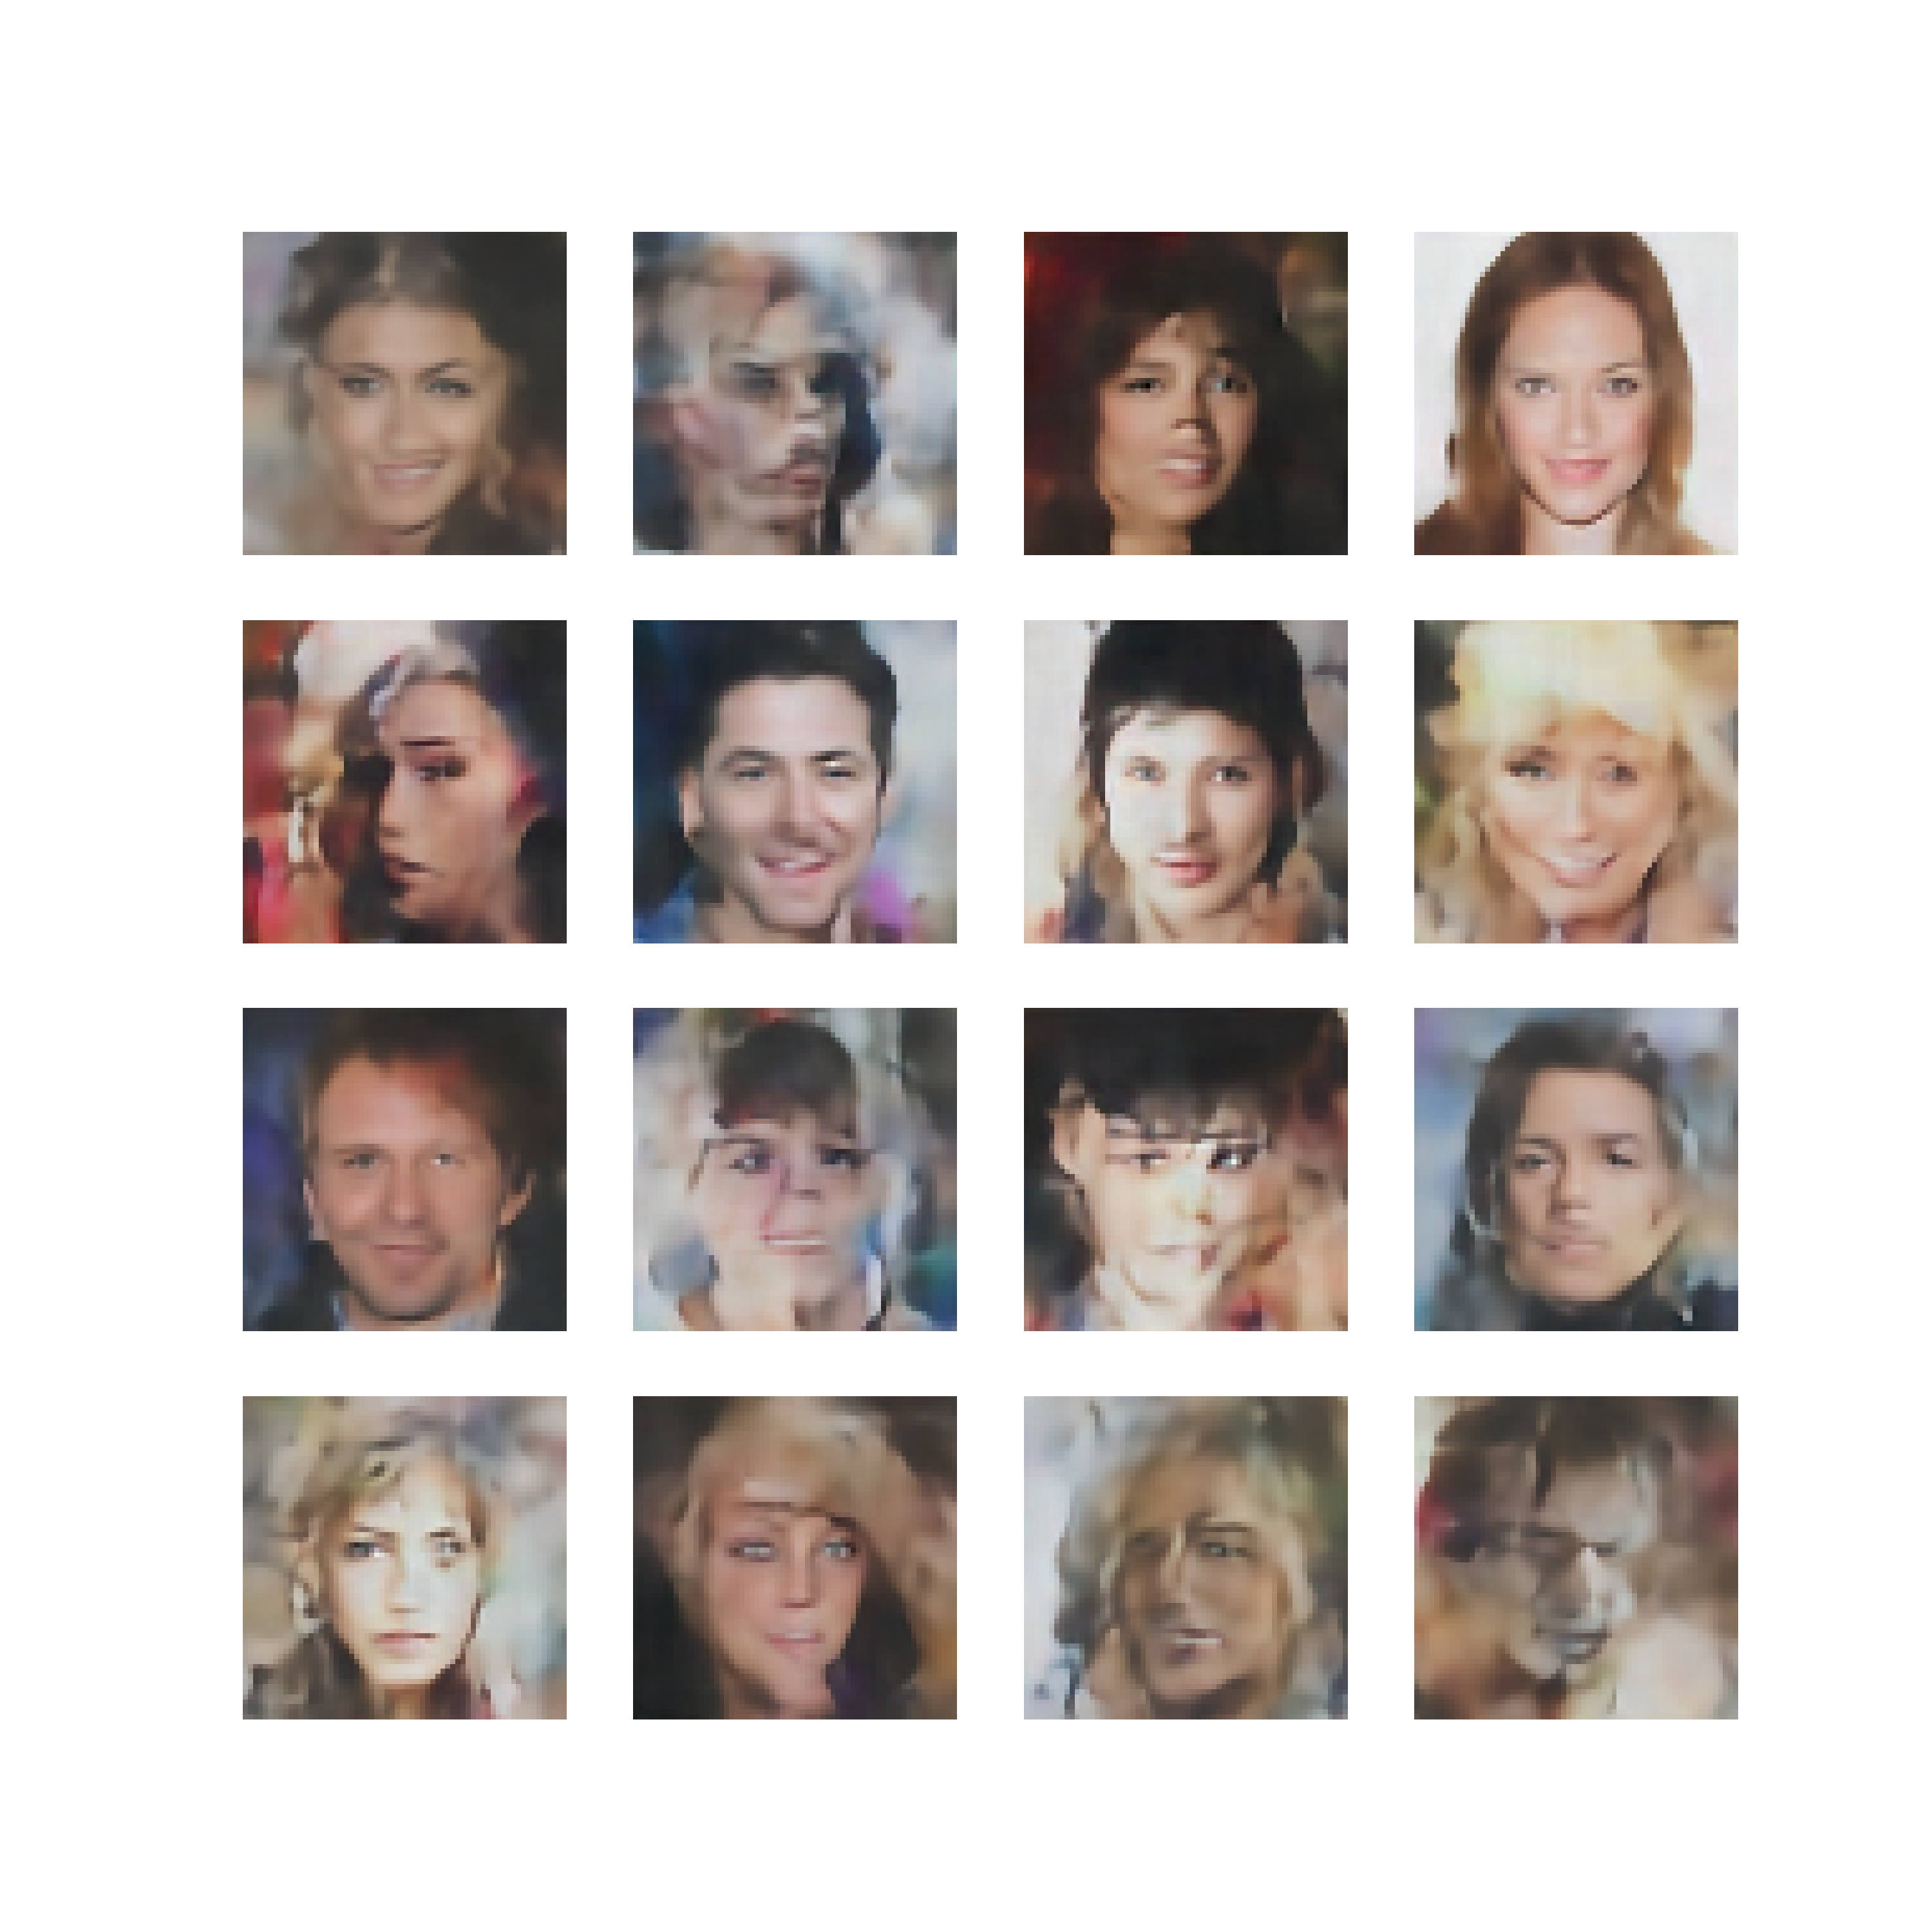
\includegraphics[width = 16cm, height = 16cm]{test_sample_3_it_4.png}
    \caption{Images generated by model.}
    \label{fig:gauss_vae}
\end{figure}
\subsection{Latent space discretisation}
\subsubsection{Model definition}
As we can see models, that we have trained so far, are not characterized by high quality image generation. However there are further enhancements, that we can apply, to improve quality of generated images. Vector Quantised-Variational AutoEncoder(VQ-VAE) \cite{VQ-VAE} \cite{VQ_VAE2} is one such method. 

The change that the model implements is latent space discretisation and increase of output tensor degree. In order to understand how VQ-VAE works we must understand output vector structure. So far it has been defined as following $q_{\phi} (\textbf{z}|\textbf{x}) = [z_1, ..., z_k], z_j\in \mathbb{R} $. As we can see, vector 
$[z_1, ..., z_k]$ can be viewed as tensor of degree one. 

The first improvement the we can apply is to increase degrees that output tensor can have. Suppose that encoder represents mapping $[h, w, c] \rightarrow [y, x, l]$. This means that encoder's input is image and encoder's output is tensor of degree 3 with dimensions $y, x, l$, where $l$ represents dimensions of latent variable . It is important to note that elements along tensor axis x and y (that is vectors defined as $[z_1, ..., z_l]$) are independent of each other.

\begin{equation}\label{eq:tensor_out}
   q_{\phi} (\textbf{z}|\textbf{x}) = 
\begin{bmatrix}
\textbf{z}^{(1,1)} &...& \textbf{z}^{(1,x)} \\
\vdots  & \vdots   & \vdots \\
\textbf{z}^{(y,1)} &...& \textbf{z}^{(y,x)} \\
\end{bmatrix}, \textbf{z} \in \mathbb{R}^{l}
.
\end{equation}
(\ref{eq:tensor_out}) visualizes tensor generated by encoder. 

In the next step, after changing  encoder's output structure, we create K-element set $ \mathcal{D} = \{\textbf{e}_1, ... \textbf{e}_{K}\}$, where  $\textbf{e}_j$ represents vector with l elements. Then we compare each vector from output tensor (along x and y axis) with elements of set $ \mathcal{D}$ and pick those elements from set $\mathcal{D}$, that are closest in sense of certain metric, we use euclidean metric. In the final step we put chosen element into their respective positions along x and y axis. The procedure can formalized as:
\begin{enumerate}
    \item $ \text{Encoder}_{\phi}(\textbf{x})  = \textbf{z}_q^{(y, x, l)}$, where y, x, l represents dimensions along given axis,
    \item $z^{(i,j)} = \text{argmin}_{p \in \{1, 2, ..., K}||\textbf{z}_q^{(i, j)} - \textbf{e}_p ||_2, $
    \item $ \textbf{z}_{index} = 
        \begin{bmatrix}
        z^{(1,1)} &...&  z^{(1,x)} \\
        \vdots  & \vdots   & \vdots \\
         z^{(y,1)} &...& z^{(y,x)} \\
    \end{bmatrix}, 
    $
    \item $\textbf{z}_\mathcal{D} =  \mathcal{D}[\textbf{z}_{index}] = 
    \begin{bmatrix}
        \textbf{z}^{(1,1)} &...& \textbf{z}^{(1,x)} \\
        \vdots  & \vdots   & \vdots \\
        \textbf{z}^{(y,1)} &...&\textbf{z}^{(y,x)} \\
    \end{bmatrix} =
    \begin{bmatrix}
        \mathcal{D}[z^{(1,1)}] &...&  \mathcal{D}[z^{(1,x)}] \\
        \vdots  & \vdots   & \vdots \\
         \mathcal{D}[z^{(y,1)}] &...& \mathcal{D}[z^{(y,x)}] \\
    \end{bmatrix}, $
    \item  $\hat{\textbf{x}} = \text{Decoder}_{\theta}(\textbf{z}_\mathcal{D}) $
\end{enumerate}
Let us define q and p distribution as following 
\begin{equation} \label{eq:vq_elem_prior}
\begin{gathered}
    q( z^{(i,j)} = k | \textbf{x}) =  
    \begin{cases}
    1 \text{ if }  k = \text{argmin}_{p \in \{1, 2, ..., K\}}||\textbf{z}_q^{i, j} - \textbf{e}_p ||_2 \\
    0 \text{ else}
    \end{cases}
\end{gathered}
,
\end{equation}
\begin{equation}
    p(z^{(i,j)}) = \text{Uniform} \{1, ... , K \}.
\end{equation}
Based on independence and (\ref{eq:vq_elem_prior}) we obtain
\begin{gather}
     q( \textbf{z}_{index} | \textbf{x}) = \prod_{i,j = 1,1}^{x, y}    
     q( z^{(i,j)} | \textbf{x}).
\end{gather}
At this point we should calculate $D_{KL}$. Suppose that $A = \{[q_1, ..., q_{yx}] \}$
represents a set of all possible $y \cdot x$-element vectors, such that $q_h \in \{ 1, 2, ..., K\}$
\begin{gather} 
    D_{KL}(q_{\phi }(\textbf{z}_{index}|\textbf{x})  || p_{\theta }(\textbf{z}_{index}) ) \\
    = \sum_{\textbf{k} \in A} q(\textbf{z}_{index} = \textbf{k} | \textbf{x}) \log\frac{q(\textbf{z}_{index} = \textbf{k} | \textbf{x})}{ p (\textbf{z}_{index}  = \textbf{k})} \\ 
     = \sum_{\textbf{k} \in A} \prod_{i,j = 1,1}^{x, y} \left[q(z^{(i,j)} = k^{ij} | \textbf{x}) \right]\log\frac{\prod_{i,j = 1,1}^{x, y} q(z^{(i,j)} = k^{ij}| \textbf{x})}
     {\prod_{i,j = 1,1}^{x, y}  p (z^{(i,j)} = k^{ij})}.
\end{gather}
Over whole set $A$ there exists exactly one element (suppose that when many smallest distance is obtained from many elements, we choose the one with lowest index) for which  
$q_{\phi }(\textbf{z}_{index}|\textbf{x}) = 1$, while for all other elements
there exists at least one pair $(g,h)$, such that $q(z^{(i,j)} = k^{ij}) = 0$. In the second case whole expression is reduced to zero. This leads us to 
\begin{gather}
    \sum_{\textbf{k} \in A}\left[ \prod_{i,j = 1,1}^{x, y}q(z^{(i,j)} = k^{ij} | \textbf{x}) \right]\log\frac{\prod_{i,j = 1,1}^{x, y} q(z^{(i,j)} = k^{ij}| \textbf{x})}
     {\prod_{i,j = 1,1}^{x, y}  p (z^{(i,j)} = k^{ij})} \\
     = \log \frac{1}{(\frac{1}{K})^{xy}} = xy\log K.
\end{gather}
$\log K$ is constant, so it has no influence on optimization. That means that $D_{KL}$ may be omitted. Additionally it is important to note that $\textbf{z}^{(i,j)} =  \mathcal{D}[z^{(i,j)}]$  is not differentiable operation, what makes encoder impossible to optimize. To solve this problem, we will copy decoder's gradient straight into decoder. This is possible because tensors $\textbf{e}_j$ and $\textbf{z}^{(i,j)}$ have the same degree and dimensions along respective axes. Loss function is defined as 
\begin{equation}
    L = \log p(\textbf{x}|\textbf{z}_\mathcal{D}) + 
    ||  sq[\text{Encoder}_{\phi}(\textbf{x})] - \textbf{e}_k||_2^2 +
    \beta || \text{Encoder}_{\phi}(\textbf{x}) - sq[\textbf{e}_k]||_2^2.
\end{equation}
A few observations:
\begin{enumerate}
    \item $sq$ stands for stop gradient, that is stopping gradient calculation for parameters within this operation,
    \item $\log p(\textbf{x}|\textbf{z}_\mathcal{D} )$ this term is knows as reconstruction error and we need to calculate it explicitly in order to optimize decoder,
    \item  $||  sq[\text{Encoder}_{\phi}(\textbf{x})] - \textbf{e}_k||_2^2 $ is used as means to optimize $\textbf{e}_k$,
    \item $\beta || \text{Encoder}_{\phi}(\textbf{x}) - sq[\textbf{e}_k]||_2^2$ is used to optimize encoder.  $\beta$ is used to prevent outpacing $\textbf{e}_j$ by encoder during optimization.
\end{enumerate}
\subsubsection{Sampling}
All that has to been done to sample VAE is to sample prior, then result of sampling insert into decoder that will output image. VQ-VAE sampling is slightly different. We can see that  tensor $\textbf{z}_{index}$
has shape $[y, x, 1]$. That means we can reshape it into vector with  $y\cdot x $ elements, to be more specific we will reorder elements of output tensor into following vector $[k_1 = z^{(1,1)},k_2 = z^{(1,2)}, ... , k_{xy} = z^{(y,x)}]$. Such vector can be used to train autoregressive neural network, the of the neural network is to predict next token in the sequence given some sequence of tokens, in VQ-VAE case network has to predict tokens until it hits   $y\cdot x $th token. Mentioned procedure can be defined as calculating conditional probability of jth token given sequence of j-1 tokens
\begin{equation}
   p(k_j) =  p(k_j | k_1, ..., k_{j-1} )
\end{equation}
Neural networks architectures used for said task can be amongst many recurrent neural networks, transformers or PixelCNN (used by VQ-VAE authors).
\begin{figure}[H]
%//\hspace*{4cm}  
    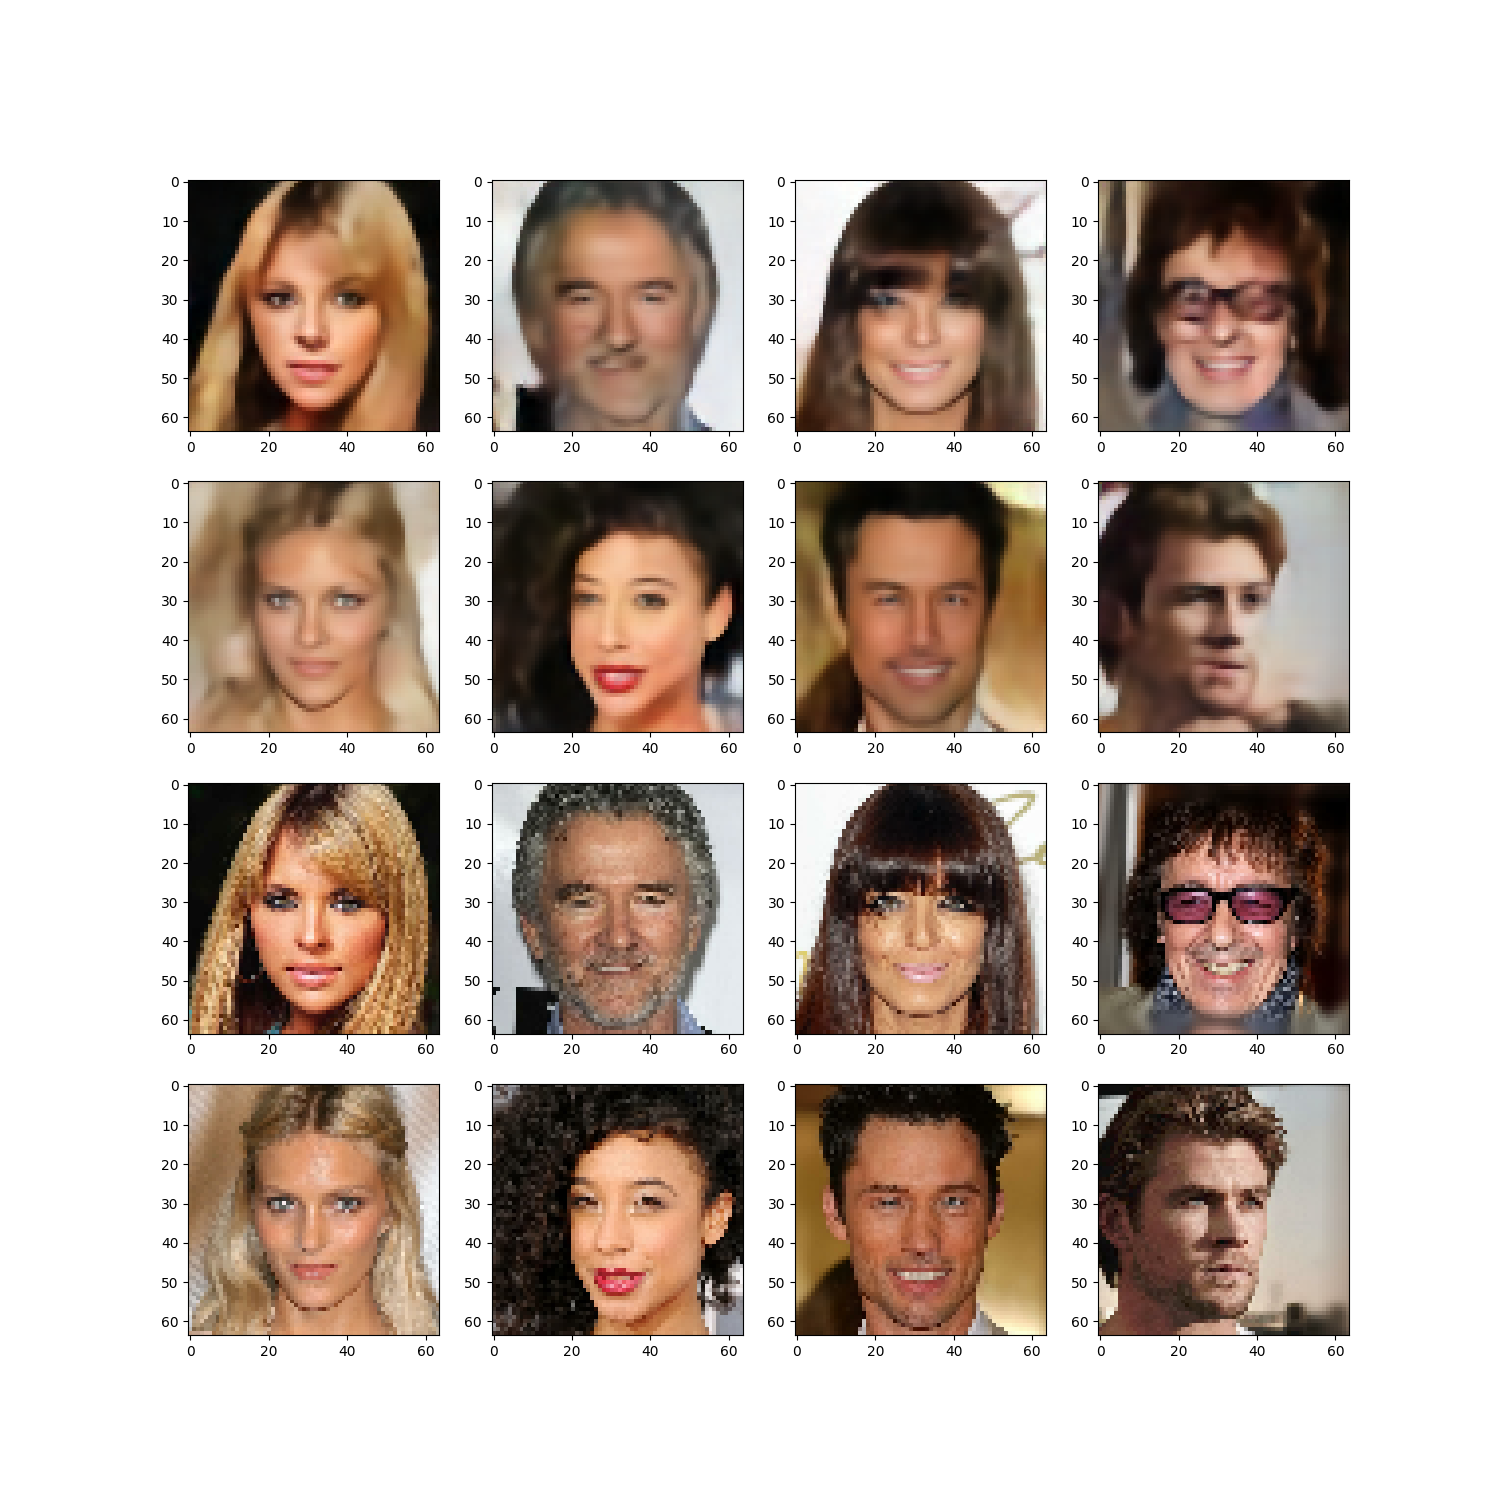
\includegraphics[width=10cm, height = 10cm]{vq_vae_img.png}
    \caption[Image reconstruction made by VQ-VAE (64x64).]
    {Image reconstruction made by VQ-VAE (64x64). Two bottom rows are original images, while two upper rows are reconstructions made by VQ-VAE.}
\end{figure}

\subsection{Summary}
In this chapter we derived equations that define behaviour and training of variational autoencoders. In the first example we created simple model that can create image that consists of binary values. Next we widened capabilities of our model by representing pixels as RGB and by allowing transformation matrix $L$ take values either below or above a diagonal.

As it can be seen, VAEs are not characterized by high quality of image generation. Characteristic trait of VAE generated image is it's blurriness (it is even seen in large architectures like DALLE-1 \cite{dalle_1}). There are further improvements that can be applied to VAE like  VQ-VAE2 \cite{VQ_VAE2} or NVAE \cite{NVAE}, that increase image quality. Yet they are still not able to beat GANs or Diffusion Models, that at the moment of writing this publication dominate image generation landscape \cite{ranking}.

VAE models advantage comes from highly flexible architecture compared to competition. It is so because VAE architecture allows to go in both ways, that is we can get latent representation of an image using encoder and reconstructed version of certain image using decoder given some latent vector. Despite lower image quality, the concept of VAE is not dead despite it's empirical flaws. In a sense diffusion models, that will be described in the next chapter, are certain limitation imposed on VAEs.

\section{Diffusion models}
Like in previous chapter, we are starting from the assumption that we have dataset 
 $\textbf{X} = [\textbf{x}_{1} , \textbf{x}_{2}, ... ,\textbf{x}_{n}]$, then we assume that $\textbf{x}_{i}$ are i.i.d  and $\textbf{x}_{i} \in \mathbb{R}^{k}$. In the case of diffusion models,
 image generation involves sampling some known distribution (for example k-dimensional gaussian) and then model's job is to denoise sample in T steps.
 \subsection{Basic definitions}
 Let $  q( \textbf{x}_{0}  ) $ represent a distribution of denoised images. Forward trajectory (forward process) with T diffusion steps is defined by distribution
 \begin{equation}
     q( \textbf{x}_{0 : T} ) = q( \textbf{x}_{0}  ) \prod_{t=1}^{T} q( \textbf{x}_{t}|  \textbf{x}_{t -1 }  ).
 \end{equation}
Reverse trajectory(reverse process) is distribution  
 \begin{equation} \label{eq:backward_proc}
     p_{\theta}( \textbf{x}_{0:T} ) = p( \textbf{x}_{T}  ) \prod_{t=1}^{T} p_{\theta}( \textbf{x}_{t-1}|  \textbf{x}_{t }  )
 \end{equation}
$q( \textbf{x}_{t}|  \textbf{x}_{t -1 }  )$ is Markov chain and $p_{\theta}( \textbf{x}_{t-1}|  \textbf{x}_{t }  )$ reverse Markov chain.
$p( \textbf{x}_{T}  )$ represents distribution that is used during sampling (like k-dimensional gauss). Role of forward process is transformation of variable with certain distribution into variable with different distribution, by adding noise at each timestep. Reverse process is reflection of forward process, it's job is to change distribution of variable by removing certain amount of noise. The goal of diffusion model is to approximate reverse model. Image generation starts with sampling $p( \textbf{x}_{T}  )$ and then iteratively, by removing noise, model tries to transform variable into variable with distribution approximately equal to the real distribution of training data.
\subsection{ELBO derivation}
Our goal is maximum likelihood estimation
 \begin{equation}
    \max_{\theta}\mathbb{E}_{q(\textbf{x}_{0})} [\log  p_{\theta}( \textbf{x}_{0}) ].
 \end{equation}
Using marginal probability in equation (\ref{eq:backward_proc}), we can express it as 
 
\begin{equation}
    p_{\theta}( \textbf{x}_{0} ) = \int p( \textbf{x}_{0:T}  ) d\textbf{x}_{1:T}.
\end{equation}
At this point we encounter a problem that distribution $ p( \textbf{x}_{t-1}|  \textbf{x}_{t }  )$ is intractable in general. That on the other hand leads as to the conclusion that $p_{\theta}( \textbf{x}_{0})$ is also intractable. Despite  $ p_{\theta}( \textbf{x}_{0} )$ being intractable in general, it is worth to note that
\begin{gather}
     p_{\theta}( \textbf{x}_{0} ) = \int p_{\theta}( \textbf{x}_{0:T}  ) d\textbf{x}_{1:T} \\
     = \int p_{\theta}( \textbf{x}_{0:T}  )  \frac{q(\textbf{x}_{1:T}|\textbf{x}_{0})}{q(\textbf{x}_{1:T}|\textbf{x}_{0})} d\textbf{x}_{1:T} \\
     =\int q(\textbf{x}_{1:T}|\textbf{x}_{0})  \frac{p_{\theta}( \textbf{x}_{0:T}  ) }{q(\textbf{x}_{1:T}|\textbf{x}_{0})} d\textbf{x}_{1:T} \\
     =\int q(\textbf{x}_{1:T}|\textbf{x}_{0}) p( \textbf{x}_{T}  )  \prod_{t=1}^{T}
     \frac{ p_{\theta}( \textbf{x}_{t-1}|  \textbf{x}_{t }  )   }
            { q( \textbf{x}_{t}|  \textbf{x}_{t -1 }  )} d\textbf{x}_{1:T} \\
    =  \mathbb{E}_{q(\textbf{x}_{1:T}|\textbf{x}_{0})}
    \Bigg[
    p( \textbf{x}_{T}  )  \prod_{t=1}^{T}
     \frac{ p_{\theta}( \textbf{x}_{t-1}|  \textbf{x}_{t }  )   }
     { q( \textbf{x}_{t}|  \textbf{x}_{t -1 }  )} d\textbf{x}_{1:T} 
    \Bigg].
\end{gather}
Using relation between min and max we get
\begin{equation}
    \max_{\theta}\mathbb{E}_{q(\textbf{x}_{0})} [\log  p_{\theta}( \textbf{x}_{0}) ] = 
    \min_{\theta}\mathbb{E}_{q(\textbf{x}_{0})} [-\log  p_{\theta}( \textbf{x}_{0}) ].
\end{equation}
To find ELBO for $ -\log  p_{\theta}( \textbf{x}_{0})$ we start from
\begin{gather}
    \mathbb{E}_{q(\textbf{x}_{0})} [-\log  p_{\theta}( \textbf{x}_{0}) ] \\
    = \int q( \textbf{x}_{0})(-1)\log  p_{\theta}( \textbf{x}_{0})d \textbf{x}_{0} \\
    = \int q( \textbf{x}_{0})(-1)\log 
    \Bigg(  \mathbb{E}_{q(\textbf{x}_{1:T}|\textbf{x}_{0})} \Bigg[
        p( \textbf{x}_{T}  )  \prod_{t=1}^{T}
     \frac{ p_{\theta}( \textbf{x}_{t-1}|  \textbf{x}_{t }  )   }
     { q( \textbf{x}_{t}|  \textbf{x}_{t -1 }  )} d\textbf{x}_{1:T}  \Bigg]
     \Bigg) d \textbf{x}_{0} \\
    = \int q( \textbf{x}_{0})(-1)\log
    \Bigg[
        \int q(\textbf{x}_{1:T}|\textbf{x}_{0}) p( \textbf{x}_{T}  )  \prod_{t=1}^{T}
         \frac{ p_{\theta}( \textbf{x}_{t-1}|  \textbf{x}_{t }  )  ) }
        { q( \textbf{x}_{t}|  \textbf{x}_{t -1 }  ))} d\textbf{x}_{1:T}
    \Bigg] 
    d \textbf{x}_{0}.
\end{gather}

\begin{Twierdzenie}[Jensen inequality] 
\label{th:jensen}
Let $X$ be a random variable and let $\phi$ be a convex function then  $\phi( \mathbb{E}[X] ) \leq \mathbb{E}[\phi(X)] $
\end{Twierdzenie}
If we set $\phi = -log$ then  $\phi$ is convex function. Based on Jensen inequality \ref{th:jensen}
we get
\begin{gather}
\int q( \textbf{x}_{0})(-1)\log
    \Bigg[
        \int q(\textbf{x}_{1:T}|\textbf{x}_{0}) p( \textbf{x}_{T}  )  \prod_{t=1}^{T}
         \frac{ p_{\theta}( \textbf{x}_{t-1}|  \textbf{x}_{t }    ) }
        { q( \textbf{x}_{t}|  \textbf{x}_{t -1 }  )} d\textbf{x}_{1:T}
    \Bigg] d \textbf{x}_{0}\\
\leq \int q( \textbf{x}_{0})q(\textbf{x}_{1:T}|\textbf{x}_{0}) (-1)\log 
\Bigg[
    p( \textbf{x}_{T}  )  \prod_{t=1}^{T}
    \frac{ p_{\theta}( \textbf{x}_{t-1}|  \textbf{x}_{t }  ) }
    { q( \textbf{x}_{t}|  \textbf{x}_{t -1 }  )}
\Bigg] d\textbf{x}_{1:T} d \textbf{x}_{0} \\
= \int q(\textbf{x}_{0:T}) (-1)\log 
\Bigg[
    p( \textbf{x}_{T}  )  \prod_{t=1}^{T}
    \frac{ p_{\theta}( \textbf{x}_{t-1}|  \textbf{x}_{t }  )   }
    { q( \textbf{x}_{t}|  \textbf{x}_{t -1 }  )}
\Bigg] d\textbf{x}_{0:T} \\ 
=    \mathbb{E}_{q(\textbf{x}_{0:T})} \Bigg[ -\log \Big( p( \textbf{x}_{T}  )  \prod_{t=1}^{T}
    \frac{ p_{\theta}( \textbf{x}_{t-1}|  \textbf{x}_{t }  )   }
    { q( \textbf{x}_{t}|  \textbf{x}_{t -1 }  )} \Big) \Bigg] \\
= \label{eq:dif_elbo_form}
\mathbb{E}_{q(\textbf{x}_{0:T})} \Bigg[ -\log p( \textbf{x}_{T}) -  \sum_{t=1}^{T}\log
    \frac{ p_{\theta}( \textbf{x}_{t-1}|  \textbf{x}_{t }  )   }
    { q( \textbf{x}_{t}|  \textbf{x}_{t -1 }  )} \Bigg].
\end{gather} 
To sum up, so far we have shown that
\begin{equation}
   \mathbb{E}_{q(\textbf{x}_{0})} [-\log  p_{\theta}( \textbf{x}_{0}) ] \leq
    \mathbb{E}_{q(\textbf{x}_{0:T})} \Bigg[ -\log p( \textbf{x}_{T}) -  \sum_{t=1}^{T}\log
    \frac{ p_{\theta}( \textbf{x}_{t-1}|  \textbf{x}_{t }  )   }
    { q( \textbf{x}_{t}|  \textbf{x}_{t -1 }  )}  \Bigg]
    = L.
\end{equation}
If we multiply by -1 we get
\begin{equation} \label{eq:elbo_diff_model}
   \mathbb{E}_{q(\textbf{x}_{0})} [\log  p_{\theta}( \textbf{x}_{0}) ] \geq
    \mathbb{E}_{q(\textbf{x}_{0:T})} \Bigg[ \log p( \textbf{x}_{T}) +  \sum_{t=1}^{T}\log
    \frac{ p_{\theta}( \textbf{x}_{t-1}|  \textbf{x}_{t }  )   }
    { q( \textbf{x}_{t}|  \textbf{x}_{t -1 }  )} ) \Bigg].
\end{equation}
Right side of equation (\ref{eq:elbo_diff_model}) we call ELBO.\\
ELBO minimization and maximization are equivalent, so to remain consistent throughout the chapter we will stick with ELBO minimization
\subsection{Finding loss function}
Suppose that:
\begin{enumerate}
\item $p(\textbf{x}_{T}) = \mathcal{N}(0, \mathbf{I})$,
\item  $p_{\theta}(\textbf{x}_{t-1}| \textbf{x}_{t}) =
        \mathcal{N}( \bm{\mu}_{\theta}(\textbf{x}_{t},t) ,\bm{\Sigma}_{\theta}(\textbf{x}_{t},t))$,
\item  $q(\textbf{x}_{t}| \textbf{x}_{t-1} ) = 
        \mathcal{N}( \sqrt{ 1 - \beta_{t}  }\textbf{x}_{t-1} ,\beta_{t}\mathbf{I} )$
        , where $\beta_t \in \{ \beta_{1}, ... , \beta_{T} \}$.
\end{enumerate}
From the above assumptions, it follows that 
\begin{Twierdzenie}\label{tw:markov_chain_gauss}
$\textbf{x}_{t} \sim  q(\textbf{x}_{t}| \textbf{x}_{0} )$  
\begin{gather*}
    \textbf{x}_{t} \sim  q(\textbf{x}_{t}| \textbf{x}_{t-1} )
    \iff
    \textbf{x}_{t} \sim  q(\textbf{x}_{t}| \textbf{x}_{0} ) = 
    \mathcal{N}( \sqrt{\overline{\alpha}_{t}} \textbf{x}_{0} , (1 - \overline{\alpha}_{t}) \mathbf{I} ), \\
    \text{for } \alpha_{t} = 1 - \beta_{t} \text{ and } \overline{\alpha}_{t} = \prod_{i=1}^{t}\alpha_{i} 
\end{gather*}
\end{Twierdzenie}
Proof: \\
Firstly we will show that$ \textbf{x}_{t} \sim  q(\textbf{x}_{t}| \textbf{x}_{t-1})
\implies
\textbf{x}_{t} \sim  q(\textbf{x}_{t}| \textbf{x}_{0} )$.
Let $\textbf{x}_{t} = [ x_{t}^{(1)}, ...  , x_{t}^{(k)} ]$ be a vector, where k represents total number of value (let l represent number of pixels o certain image then  k=l, however if said image was RGB with the same number of pixels then k = 3*l). It is important to note that $x_{t}^{(i)}$ are independent of each other. From
$\textbf{x}_{t} \sim \mathcal{N}( \sqrt{ \alpha_{t} }\textbf{x}_{t-1} ,(1 - \alpha_{t}) \mathbf{I} ) $ it follows that each element of vector $x_{t}^{(i)}$ has the same variance and scaling factor  $ \sqrt{ \alpha_{t} }$. These properties allows us to consider each $x_{t}^{(i)}$ separately and then generalize result to other elements of vector $\textbf{x}_{t}$.


 From properties of normal distribution it follows that if $ \epsilon \sim  \mathcal{N}(0, 1) $  then $x_{t}$ ((i) shall be omitted to improve clarity) can be expressed as
\begin{gather} \label{eq:rec_proof_start}
    x_{t} =  \sqrt{  \alpha_{t} } x_{t-1}  + \sqrt{ 1 - \alpha_{t}}\epsilon_{t-1} \\
    = 
     \label{eq:rec_proof}
    \sqrt{  \alpha_{t} } (\sqrt{  \alpha_{t-1} } x_{t-2}  + \sqrt{ 1 - \alpha_{t-1}}\epsilon_{t-2}) 
    + \sqrt{ 1 - \alpha_{t}}\epsilon_{t-1} \\
    = \sqrt{  \alpha_{t} } \sqrt{  \alpha_{t-1} } x_{t-2} + 
        \sqrt{  \alpha_{t} } \sqrt{ 1 - \alpha_{t-1}}\epsilon_{t-2}
         + \sqrt{ 1 - \alpha_{t}}\epsilon_{t-1}.
\end{gather}
\begin{Twierdzenie}[Sum of gaussian.]\label{gaussian_sum_dist}
Let X i Y be independent random variables with normal distribution. Sum of those variables is also normally distributed that is, if
\begin{enumerate}
   \item   $X \sim \mathcal{N}( \mu_{X}, \sigma_{X}^{2})$
    \item  $Y \sim \mathcal{N}( \mu_{Y}, \sigma_{Y}^{2})$
    \item   $Z = X + Y$
\end{enumerate}
then
\begin{displaymath}
   Z \sim \mathcal{N}( \mu_{X} +\mu_{Y} , \sigma_{X}^{2} + \sigma_{Y}^{2} ).
\end{displaymath}

\end{Twierdzenie}
We note that
\begin{equation}
    \sqrt{  \alpha_{t} } \sqrt{  \alpha_{t-1} } x_{t-2} + 
        \sqrt{  \alpha_{t} } \sqrt{ 1 - \alpha_{t-1}}\epsilon_{t-2}
         + \sqrt{ 1 - \alpha_{t}}\epsilon_{t-1},
\end{equation}
can be interpreted as
\begin{gather}
      Z = X + Y,
\end{gather}
then
\begin{gather}
    X \sim \mathcal{N}( \sqrt{  \alpha_{t} } \sqrt{  \alpha_{t-1} } x_{t-2},  \alpha_{t}( 1 - \alpha_{t-1}) ), \\
    Y \sim \mathcal{N}(0 ,  1 - \alpha_{t}).
\end{gather}
Based on theorem \ref{gaussian_sum_dist} we get 
\begin{equation}
     x_{t} \sim \mathcal{N}( \sqrt{  \alpha_{t} \alpha_{t-1} } x_{t-2}, 1 - \alpha_{t}\alpha_{t-1} ),
\end{equation}
what leads us to
\begin{gather}
    x_{t} = \sqrt{  \alpha_{t} \alpha_{t-1} } x_{t-2} + \sqrt{1 - \alpha_{t}\alpha_{t-1}} \epsilon_{t-2} \\
    =  \sqrt{  \alpha_{t} \alpha_{t-1} } 
    (\sqrt{  \alpha_{t} } x_{t-3}  + \sqrt{ 1 - \alpha_{t}}\epsilon_{t-3})
    + \sqrt{1 - \alpha_{t}\alpha_{t-1}} \epsilon_{t-2}.
\end{gather}
If we apply substitution  $\overline{\alpha}_{t:k} = \alpha_{t} \cdot ... \cdot \alpha_{k}$ we obtain  
\begin{equation}
    x_{t} =  \sqrt{  \overline{\alpha}_{t:t-1} } 
    (\sqrt{  \alpha_{t-2} } x_{t-3}  + \sqrt{ 1 - \alpha_{t-2}}\epsilon_{t-3})
    + \sqrt{1 - \overline{\alpha}_{t:t-1}} \epsilon_{t-2}.
\end{equation}
We can note that above equation is similar to (\ref{eq:rec_proof}),
from formulas we can conclude that (\ref{eq:rec_proof_start}) has recursive structure. We can apply aforementioned substitution until we hit  $x_{0}$, what leads us to equation
\begin{equation} \label{eq:x_t_sample}
    x_{t} =  \sqrt{\overline{\alpha}_{t:1}  }x_{0} + \sqrt{1 - \overline{\alpha}_{t:1}} \epsilon_{1}.
\end{equation}
From (\ref{eq:x_t_sample}) it follows that 
\begin{equation}
     x_{t} \sim \mathcal{N}( \sqrt{\overline{\alpha}_{t:1}  }x_{0}, 1 - \overline{\alpha}_{t:1}).
\end{equation}
Based on independence of  $x_{t}^{(i)}$ we can conclude the first part of the proof by stating that
\begin{equation}
    \textbf{x}_{t} \sim 
    \mathcal{N}( \sqrt{\overline{\alpha}_{t}  }\textbf{x}_{0}, (1 - \overline{\alpha}_{t} \mathbf{I}) ).
\end{equation}
In order to prove $ \textbf{x}_{t} \sim  q(\textbf{x}_{t}| \textbf{x}_{0})
\implies
\textbf{x}_{t} \sim  q(\textbf{x}_{t}| \textbf{x}_{t-1} )$ above reasong should be applied in exactly reversed order, what concludes the proof. $\blacksquare$ \\
At this point we will to transform ELBO to a form, that can be effectively use during neural network training. 
\begin{gather}
     \mathbb{E}_{q(\textbf{x}_{0:T})} \Bigg[ -\log p( \textbf{x}_{T}) -  \sum_{t=1}^{T}\log
    \frac{ p_{\theta}( \textbf{x}_{t-1}|  \textbf{x}_{t }  )   }
    { q( \textbf{x}_{t}|  \textbf{x}_{t -1 }  )} ) \Bigg] \\
    = \mathbb{E}_{q(\textbf{x}_{0:T})} \Bigg[ -\log p( \textbf{x}_{T}) -  \sum_{t=2}^{T}\log
    \frac{ p_{\theta}( \textbf{x}_{t-1}|  \textbf{x}_{t }  )   }
    { q( \textbf{x}_{t}|  \textbf{x}_{t -1 }  )} - \log
    \frac{ p_{\theta}( \textbf{x}_{0}|  \textbf{x}_{1}  )   }
    { q( \textbf{x}_{1}|  \textbf{x}_{0}  )}
    \ \Bigg].
\end{gather}
As $ q( \textbf{x}_{t}|  \textbf{x}_{t -1 })$ is Markov process, we can additionally condition distribution on $\textbf{x}_{0}$,
that is $ q( \textbf{x}_{t}|  \textbf{x}_{t -1},\textbf{x}_{0} )$. 
Then using Bayes rule we obtain
\begin{equation}
    q( \textbf{x}_{t}|  \textbf{x}_{t -1 },  \textbf{x}_{0}) = 
    \frac{ q( \textbf{x}_{t-1}|  \textbf{x}_{t},  \textbf{x}_{0}) q( \textbf{x}_{t}| \textbf{x}_{0})}
    {q( \textbf{x}_{t-1}| \textbf{x}_{0})},
\end{equation}
what leads us to
\begin{gather}
    \begin{gathered}
    \mathbb{E}_{q(\textbf{x}_{0:T})} \Bigg[ -\log p( \textbf{x}_{T}) - \\ \sum_{t=2}^{T}\log
    \frac{ p_{\theta}( \textbf{x}_{t-1}|  \textbf{x}_{t }  )   }
    { q( \textbf{x}_{t-1}|  \textbf{x}_{t},  \textbf{x}_{0}  )}
    \frac{q( \textbf{x}_{t-1}|  \textbf{x}_{0})}{q( \textbf{x}_{t}|  \textbf{x}_{0})} - \\ \log
    \frac{ p_{\theta}( \textbf{x}_{0}|  \textbf{x}_{1}  )   }
    { q( \textbf{x}_{1}|  \textbf{x}_{0}  )}
    \ \Bigg]
    \end{gathered}
    \\
    =  \mathbb{E}_{q(\textbf{x}_{0:T})} 
    \Bigg[ -\log \frac{p( \textbf{x}_{T})}{q( \textbf{x}_{T}|  \textbf{x}_{0})} -  \sum_{t=2}^{T}\log
    \frac{ p_{\theta}( \textbf{x}_{t-1}|  \textbf{x}_{t }  )   }
    { q( \textbf{x}_{t-1}|  \textbf{x}_{t},  \textbf{x}_{0}  )}
    -\log  p_{\theta}( \textbf{x}_{0}|  \textbf{x}_{1}  )    \Bigg] \\
    \begin{gathered}
    =\label{eq:main_elbo}
    \mathbb{E}_{q(\textbf{x}_{0:T})} 
    \Bigg[ -\log \frac{p( \textbf{x}_{T})}{q( \textbf{x}_{T}|  \textbf{x}_{0})}\Bigg]
    \\+ \sum_{t=2}^{T} \mathbb{E}_{q(\textbf{x}_{0:T})}  
    \Bigg[  -\log
    \frac{ p_{\theta}( \textbf{x}_{t-1}|  \textbf{x}_{t }  )   }
    { q( \textbf{x}_{t-1}|  \textbf{x}_{t},  \textbf{x}_{0}  )}\Bigg]
    \\- \mathbb{E}_{q(\textbf{x}_{0:T})} 
    \Bigg[\log  p_{\theta}( \textbf{x}_{0}|  \textbf{x}_{1}  )    \Bigg] .
    \end{gathered}
\end{gather}
Transformation of the first and last term in equation (\ref{eq:main_elbo}) is trivial so we will skip it, however middle term is more complex to transform so we will focus on it. Firtly middle term can be expanded for certain t
\begin{gather}
\mathbb{E}_{q(\textbf{x}_{0:T})}  
    \Bigg[ -\log
    \frac{ p_{\theta}( \textbf{x}_{t-1}|  \textbf{x}_{t }  )   }
    { q( \textbf{x}_{t-1}|  \textbf{x}_{t},  \textbf{x}_{0}  )}\Bigg] \\
    \begin{gathered}
    = \int q(\textbf{x}_{0})q(\textbf{x}_{t-1}|\textbf{x}_{t-2})q(\textbf{x}_{t}|\textbf{x}_{t-1}, \textbf{x}_{0})
   \\ \Bigg[ -\log \frac{ p_{\theta}( \textbf{x}_{t-1}|  \textbf{x}_{t }  )   }
    { q( \textbf{x}_{t-1}|  \textbf{x}_{t},  \textbf{x}_{0}  )}\Bigg] \\
    d \textbf{x}_{0} d \textbf{x}_{t-1} d \textbf{x}_{t}. 
    \end{gathered}
\end{gather}
Using Bayes theorem gives  $q(\textbf{x}_{t}|\textbf{x}_{t-1}, \textbf{x}_{0}) = \frac{ q( \textbf{x}_{t-1}|  \textbf{x}_{t}, \textbf{x}_{0}) q( \textbf{x}_{t}| \textbf{x}_{0})}
    {q( \textbf{x}_{t-1}| \textbf{x}_{0})}
    $. From theroem \ref{tw:markov_chain_gauss} it follows that $\textbf{x}_{t-1} \sim  q(\textbf{x}_{t-1}| \textbf{x}_{0} ) $ is equivalent to
$\textbf{x}_{t-1} \sim  q(\textbf{x}_{t-1}| \textbf{x}_{t-2} ) $, what yields us
\begin{gather}
    \begin{gathered}
\int q(\textbf{x}_{0})q(\textbf{x}_{t-1}|\textbf{x}_{t-2})
\frac{ q( \textbf{x}_{t-1}|  \textbf{x}_{t}, \textbf{x}_{0}) q( \textbf{x}_{t}| \textbf{x}_{0})}
    {q( \textbf{x}_{t-1}| \textbf{x}_{t-2})}\\
    \Bigg[  -\log \frac{ p_{\theta}( \textbf{x}_{t-1}|  \textbf{x}_{t }  )   }
    { q( \textbf{x}_{t-1}|  \textbf{x}_{t},  \textbf{x}_{0}  )}\Bigg] 
    d \textbf{x}_{0} d \textbf{x}_{t-1} d \textbf{x}_{t} 
        \end{gathered}\\
    = \int q(\textbf{x}_{0})q( \textbf{x}_{t}| \textbf{x}_{0})q( \textbf{x}_{t-1}|  \textbf{x}_{t})
      \Bigg[ -\log \frac{ p_{\theta}( \textbf{x}_{t-1}|  \textbf{x}_{t }  )   }
    { q( \textbf{x}_{t-1}|  \textbf{x}_{t},  \textbf{x}_{0}  )}\Bigg] 
    d \textbf{x}_{0} d \textbf{x}_{t-1} d \textbf{x}_{t} \\
    =\int  q(\textbf{x}_{0}, \textbf{x}_{t})  \Bigg[\int q( \textbf{x}_{t-1}|  \textbf{x}_{t},  \textbf{x}_{0})
        (-1)\log \frac{ p_{\theta}( \textbf{x}_{t-1}|  \textbf{x}_{t }  )   }
    { q( \textbf{x}_{t-1}|  \textbf{x}_{t},  \textbf{x}_{0}  )}
    d \textbf{x}_{t-1} \Bigg] d \textbf{x}_{0}d \textbf{x}_{t} \\
    = \int  q(\textbf{x}_{0}, \textbf{x}_{t}) 
    D_{KL}\big( q( \textbf{x}_{t-1}|  \textbf{x}_{t},  \textbf{x}_{0})||
    p_{\theta}( \textbf{x}_{t-1} | \textbf{x}_{t} ) \big)
    d \textbf{x}_{0}d \textbf{x}_{t} \\
    =\label{eq:dkl_loss}
    \mathbb{E}_{q(\textbf{x}_{0}, \textbf{x}_{t})}  \Bigg[
    D_{KL}\big( q( \textbf{x}_{t-1}|  \textbf{x}_{t},  \textbf{x}_{0})||
    p_{\theta}( \textbf{x}_{t-1} | \textbf{x}_{t} ) \big)
    \Bigg].
\end{gather}
By substituting (\ref{eq:dkl_loss})  into mid term of equation (\ref{eq:main_elbo}) we obtain
\begin{gather}
\begin{gathered} \label{eq:eblo_main}
     L_{vlb} = \mathbb{E}_{q(\textbf{x}_{0})}
     \Bigg[ D_{KL}\big( q( \textbf{x}_{T}|  \textbf{x}_{0})|| p( \textbf{x}_{T}) \big)  \Bigg] \\
     + \sum_{t=2}^{T}\mathbb{E}_{q(\textbf{x}_{0}, \textbf{x}_{t})}
       \Bigg[ D_{KL}\big( q( \textbf{x}_{t-1}|  \textbf{x}_{t},  \textbf{x}_{0})|| p_{\theta}( \textbf{x}_{t-1} | \textbf{x}_{t} ) \big)  \Bigg] \\
        - \mathbb{E}_{q(\textbf{x}_{0}, \textbf{x}_{1})} 
    \Bigg[\log  p_{\theta}( \textbf{x}_{0}|  \textbf{x}_{1}  )    \Bigg].
\end{gathered}
\end{gather}
We can see that equation (\ref{eq:eblo_main}) can be split into three parts:
\begin{enumerate}
    \item $L_{T} = \mathbb{E}_{q(\textbf{x}_{0})} 
     \Bigg[ D_{KL}\big( q( \textbf{x}_{T}|  \textbf{x}_{0})|| p( \textbf{x}_{T}) \big)  \Bigg]$\\
     This expression compares a distribution of forward process after T steps with a distribution from which we sample in order to create new image. 
     Fact that $D_{KL} \geq 0$ leads us to the conclusion, that optimization of $L$ requires   $q$ and $p$ to be as close as possible.
    \item $ L_{t-1} = \mathbb{E}_{q(\textbf{x}_{0}, \textbf{x}_{t})}
       \Bigg[ D_{KL}\big( q( \textbf{x}_{t-1}|  \textbf{x}_{t},  \textbf{x}_{0})|| p_{\theta}( \textbf{x}_{t-1} | \textbf{x}_{t} ) \big)  \Bigg]$\\
       This term controls, how well we are able to reverse process of injecting noise into certain image. $q( \textbf{x}_{t-1}|  \textbf{x}_{t},  \textbf{x}_{0})$ can be interpreted as a distribution of images that were injected noise t-1 times, from which distribution of images with injected noise t times is created. $p_{\theta}( \textbf{x}_{t-1} | \textbf{x}_{t} )$ represents our model,  whose goal is to denoise image at t-th step. 
    \item  $ L_{0} = -\mathbb{E}_{q(\textbf{x}_{0}, \textbf{x}_{1})} 
    \Bigg[\log  p_{\theta}( \textbf{x}_{0}|  \textbf{x}_{1}  )    \Bigg] $ \\
    This expression is called reconstruction loss.
\end{enumerate}
\subsection{Denoising diffusion model}
Our optimization objective is minimization of equation (\ref{eq:eblo_main}).
In order to make calculations more readable the equation shall be split into three separate parts, and once transformations are done, put back together 
\subsubsection{$L_T$}
$L_{T}$ is defined arbitrarily and does not depend on  $\theta$,
additionally elements of a sequence $\beta$ are also constant, so this term can be ignored. 
\subsubsection{$L_{t-1}$}
Suppose that
$p_{\theta}(\textbf{x}_{t-1} | \textbf{x}_{t}) = \mathcal{N}
(\bm{\mu}_{\theta}(\textbf{x}_{t}, t), \sigma^2_t \mathbf{I} )$, where $\sigma^2_t$ is constant and depends on time t. Before Kullback-Leibler divergence can be determined, distribution $q( \textbf{x}_{t-1}|  \textbf{x}_{t},  \textbf{x}_{0})$ must be found.
\begin{gather}
q( \textbf{x}_{t-1}|  \textbf{x}_{t},  \textbf{x}_{0}) =
\frac{q( \textbf{x}_{t}|  \textbf{x}_{t-1},  \textbf{x}_{0}) q( \textbf{x}_{t-1}|\textbf{x}_{0})}
{q( \textbf{x}_{t}|\textbf{x}_{0})} \\ 
= \frac{
    \mathcal{N}(\textbf{x}_{t}; \sqrt{\alpha_{t}} \textbf{x}_{t-1}, (1 - \alpha_{t})\mathbf{I}) 
    \mathcal{N}(\textbf{x}_{t-1}; \sqrt{\overline{\alpha}_{t-1}} \textbf{x}_{0}, (1 - \overline{\alpha}_{t-1})\mathbf{I})
    }{
     \mathcal{N}(\textbf{x}_{t}; \sqrt{\overline{\alpha}_{t}} \textbf{x}_{t}, (1 - \overline{\alpha_{t}})\mathbf{I})
    }.
\end{gather}
It is important to note that each elements of vector $\textbf{x}_{t}$ are independent of each other, this fact makes it possible to write that
\begin{gather}
q( \textbf{x}_{t-1}|  \textbf{x}_{t},  \textbf{x}_{0}) = \\
    \frac{
  \mathcal{N}_{1:l}(x_{t};\sqrt{\alpha_{t}} x_{t}, 1 - \alpha_{t-1}) 
  \mathcal{N}_{1:l}(x_{t-1};\sqrt{\alpha_{t-1}} x_{0}, 1 -  \overline{\alpha}_{t-1} ) 
  }{
    \mathcal{N}_{1:l}(x_{t};\sqrt{\alpha_{t}} x_{0}, 1 - \overline{\alpha}_{t}) ,
  }
\end{gather}
where $ \mathcal{N}_{1:l} = \mathcal{N}_{1} \cdot ... \cdot \mathcal{N}_{l} $.
 Product   $ \mathcal{N}_{1:l}$ can be grouped in such a way, that for i-th element of vector $\textbf{x}_{t}$, it's distribution can be expressed as
\begin{gather}
q_{i}( x_{t-1}|  x_{t}, x_{0})   = 
\frac{
  \mathcal{N}_{i}(x_{t};\sqrt{\alpha_{t}} x_{t-1}, 1 - \alpha_{t-1}) 
  \mathcal{N}_{i}(x_{t-1};\sqrt{\overline{\alpha}_{t}} x_{0}, 1 - \alpha_{t}) 
  }{
    \mathcal{N}_{i}(x_{t};\sqrt{\alpha_{t}} x_{0}, 1 - \alpha_{t}) 
  } \\ 
\propto \exp \Big( -\frac{1}{2}\Big[ 
\frac{(x_t - \sqrt{ \alpha_{t}} x_{t-1})^{2} }{1 - \alpha_{t}} + 
\frac{(x_{t-1} - \sqrt{ \overline{\alpha}_{t-1}} x_{0})^{2} }{1 - \overline{\alpha}_{t-1}} -
\frac{(x_t - \sqrt{\overline{\alpha}_{t}} x_{0})^{2} }{1- \overline{\alpha}_{t}}
\Big]\Big) \\ 
= \exp \Big( -\frac{1}{2}\Big[ 
\frac{ -2\sqrt{ \alpha_{t}} x_{t-1} x_t + \alpha_{t}x_{t-1}^{2} }{1 - \alpha_{t}} + 
\frac{x_{t-1}^{2} - 2\sqrt{ \overline{\alpha}_{t-1}}x_{t-1}x_{0} }{1 - \overline{\alpha}_{t-1}}+
C(x_t, x_0)
\Big]\Big) 
\end{gather} 
where $C(x_t, x_0) = x_t^2 - \overline{\alpha}_{t-1}x_0^2 +
\frac{(x_t - \sqrt{\overline{\alpha}_{t}} x_{0})^{2} }{1- \overline{\alpha}_{t}}$
\begin{gather} 
\propto \exp \Big( -\frac{1}{2}\Big[ 
\frac{ -2\sqrt{ \alpha_{t}} x_{t-1} x_t + \alpha_{t}x_{t-1}^{2} }{1 - \alpha_{t}} + 
\frac{x_{t-1}^{2} - 2\sqrt{ \overline{\alpha}_{t-1}}x_{t-1}x_{t-1} }{1 - \overline{\alpha}_{t-1}}
\Big]\Big) \\
= \exp \Big( -\frac{1}{2}\Big[ 
\Big( \frac{\alpha_{t}}{1 - \alpha_{t}} + \frac{1}{1-\overline{\alpha}_{t-1}} \Big) x_{t-1}^2 -
2\Big( \frac{\sqrt{ \alpha_{t}} x_{t}}{1 - \alpha_{t}} +
\frac{\sqrt{ \overline{\alpha}_{t-1}} x_{0}}{1-\overline{\alpha}_{t-1}}   \Big) x_{t-1} 
\Big]\Big)  \\
= \exp \Big( -\frac{1}{2}\Big[ 
\frac{1 - \overline{\alpha}_t }{(1 - \alpha_{t})(1-\overline{\alpha}_{t-1})} x_{t-1}^2 -
2\frac{\sqrt{ \alpha_{t}}(1-\overline{\alpha}_{t-1}) x_{t} + 
\sqrt{ \overline{\alpha}_{t-1}}(1 - \alpha_{t}) x_{0} }
{(1 - \alpha_{t})(1-\overline{\alpha}_{t-1})} x_{t-1} 
\Big]\Big) \\
=  \exp \Big( -\frac{1}{2}
\frac{1}{\frac{(1 - \alpha_{t})(1-\overline{\alpha}_{t-1})}{1 - \overline{\alpha}_t }} \Big[ 
 x_{t-1}^2 -
2\frac{\sqrt{ \alpha_{t}}(1-\overline{\alpha}_{t-1}) x_{t} + 
\sqrt{ \overline{\alpha}_{t-1}}(1 - \alpha_{t}) x_{0} }
{1-\overline{\alpha}_{t}} x_{t-1} 
\Big]\Big) \\
\propto 
\exp \Big( -\frac{1}{2}
\frac{1}{\frac{(1 - \alpha_{t})(1-\overline{\alpha}_{t-1})}{1 - \overline{\alpha}_t }} \Big[ 
 x_{t-1}^2 -
2\frac{\sqrt{ \alpha_{t}}(1-\overline{\alpha}_{t-1}) x_{t} + 
\sqrt{ \overline{\alpha}_{t-1}}(1 - \alpha_{t}) x_{0} }
{1-\overline{\alpha}_{t}} x_{t-1} 
\Big]\Big) \exp(C).
\end{gather}
Assume that
$C = \frac{1}{\frac{(1 - \alpha_{t})(1-\overline{\alpha}_{t-1})}{1 - \overline{\alpha}_t }}
\frac{\sqrt{ \alpha_{t}}(1-\overline{\alpha}_{t-1}) x_{t} + 
\sqrt{ \overline{\alpha}_{t-1}}(1 - \alpha_{t}) x_{0} }
{1-\overline{\alpha}_{t}}$, from the assumption it follows that
\begin{gather}
\mathcal{N} \Big(
x_{t-1};
\frac{\sqrt{ \alpha_{t}}(1-\overline{\alpha}_{t-1}) x_{t} + 
\sqrt{ \overline{\alpha}_{t-1}}(1 - \alpha_{t}) x_{0} }
{1-\overline{\alpha}_{t}} ,
\frac{(1 - \alpha_{t})(1-\overline{\alpha}_{t-1}), }{1 - \overline{\alpha}_t }
\Big).
\end{gather} 
Above calculations can be applied for each of l variables. Writing result of above calculations in vector notation yields 
\begin{equation}
    \textbf{x}_{t-1} \sim \mathcal{N} \Big(
\frac{\sqrt{ \alpha_{t}}(1-\overline{\alpha}_{t-1}) \textbf{x}_{t} + 
\sqrt{ \overline{\alpha}_{t-1}}(1 - \alpha_{t})  \textbf{x}_{0} }
{1-\overline{\alpha}_{t}} ,
\frac{(1 - \alpha_{t})(1-\overline{\alpha}_{t-1}), }{1 - \overline{\alpha}_t} \mathbf{I}
\Big).
\end{equation}
In order to keep clarity of following calculations, mean and variance will be denoted as 
$\bm{\mu}(\textbf{x}_{t}, \textbf{x}_{0})$ i
$\overline{\beta}_t$ respectively.
Finding distribution $q( \textbf{x}_{t-1}|  \textbf{x}_{t},  \textbf{x}_{0})$ allows to explicitly calculate Kullback–Leibler divergence
\begin{gather}
    D_{KL}\big( q( \textbf{x}_{t-1}|  \textbf{x}_{t},  \textbf{x}_{0})|| p_{\theta}( \textbf{x}_{t-1} | \textbf{x}_{t} ) \big) \\
    = D_{KL}\big( \mathcal{N}_q | \mathcal{N}_p ) \big) \\
    \begin{gathered}
    =\frac{1}{2} \Big[
    (\bm{\mu}_{\theta}(\textbf{x}_{t}, t) -  \bm{\mu}(\textbf{x}_{t}, \textbf{x}_{0}))^T
    (\sigma^2_T \mathbf{I})^{-1}
    (\bm{\mu}_{\theta}(\textbf{x}_{t}, t) -  \bm{\mu}(\textbf{x}_{t}, \textbf{x}_{0}))\\
     - \text{tr} (\sigma^2_T \mathbf{I}^{-1} \overline{\beta}_t\mathbf{I})  
     -k
     + \log \frac{|\sigma^2_T \mathbf{I}|}{|\overline{\beta}_t\mathbf{I}|}
     \Big]\end{gathered} \\
     = \frac{1}{2} \Big[
     \frac{1}{\sigma^2_t} ||\bm{\mu}_{\theta}(\textbf{x}_{t}, t) -  \bm{\mu}(\textbf{x}_{t}, \textbf{x}_{0})||^2
     + Const
     \Big] \\
     = \frac{1}{2\sigma^2_t}
     ||\bm{\mu}_{\theta}(\textbf{x}_{t}, t) -  \bm{\mu}(\textbf{x}_{t}, \textbf{x}_{0})||^2 + Const
\end{gather}
$Const$ can be omitted, so the result comes down to
\begin{equation}
    L_{t-1} =   \mathbb{E}_{q(\textbf{x}_{0}, \textbf{x}_{t})} \Big[ \frac{1}{2\sigma^2_t}
    ||\bm{\mu}_{\theta}(\textbf{x}_{t}, t) -  \bm{\mu}(\textbf{x}_{t}, \textbf{x}_{0})||^2 \Big].
\end{equation}
From the fact 
\begin{gather}
\textbf{x}_{t} = \sqrt{\overline{\alpha}_t}\textbf{x}_{0} + \sqrt{1 - \overline{\alpha}_t}\bm{\epsilon}
\text{ for } \bm{\epsilon} \sim \mathcal{N}(0, \mathbf{I}) \\
\iff  \frac{1}{\sqrt{\overline{\alpha}_t}}
(\textbf{x}_{t} - \sqrt{1 - \overline{\alpha}_t}\bm{\epsilon} )  = \textbf{x}_{0} 
\text{ for } \bm{\epsilon} \sim \mathcal{N}(0, \mathbf{I}),
\end{gather}
it follows that
\begin{gather}
        L_{t-1} =   \mathbb{E}_{q(\textbf{x}_{0}, \textbf{x}_{t})} \Big[ \frac{1}{2\sigma^2_t}
    ||\bm{\mu}_{\theta}(\textbf{x}_{t}, t) -  \bm{\mu}(\textbf{x}_{t}, 
    \frac{1}{\sqrt{\overline{\alpha}_t}}(\textbf{x}_{t} - \sqrt{1 - \overline{\alpha}_t}\bm{\epsilon} )
    )||^2 \Big] \\
    = \label{eq:norm_ddm}
    \mathbb{E}_{q(\textbf{x}_{0}, \textbf{x}_{t})} \Big[ 
    \frac{1}{2\sigma^2_t}
    ||\hat{\bm{\mu}}_{\theta}(\textbf{x}_{t}, t) -  
    \frac{1}{\sqrt{\alpha_t}}\Big(\textbf{x}_t - \frac{1 - \alpha_t}{\sqrt{1 - \overline{\alpha}_t}}\bm{\epsilon} \Big) ||^2 \Big]. 
\end{gather}
Second term from equation (\ref{eq:norm_ddm}) is objective, that model should be able to predict. As  $\hat{\bm{\mu}}_{\theta}$ can be chosen arbitrarily, suppose that
\begin{equation} \label{eq:elbo_mean}
    \hat{\bm{\mu}}_{\theta}(\textbf{x}_{t}, t) =  \frac{1}{\sqrt{\alpha_t}}\Big(\textbf{x}_t - \frac{1 - \alpha_t}{\sqrt{1 - \overline{\alpha}_t}}\bm{\epsilon}_{\theta}(\textbf{x}_{t}, t) \Big),
\end{equation}
where  $\bm{\epsilon}_{\theta}$ denotes neural network. Result of the substitution is
\begin{gather}
      L_{t-1} =   \mathbb{E}_{q(\textbf{x}_{0}, \textbf{x}_{t})} \Big[
      \frac{(1-\alpha_t)^2}{2\sigma^2_t \alpha_t (1-\overline{\alpha}_t)}
       ||\bm{\epsilon}_{\theta}(\textbf{x}_{t}, t) - \bm{\epsilon} ||^2
      \Big]
\end{gather}
Applying reparametrization trick for $\textbf{x}_t$ yields
\begin{gather}
      L_{t-1} =   \mathbb{E}_{q(\textbf{x}_{0})}\Big(  \mathbb{E}_{q(\textbf{x}_{t}|\textbf{x}_{0} )} \Big[
      \frac{(1-\alpha_t)^2}{2\sigma^2_t \alpha_t (1-\overline{\alpha}_t)}
       ||\bm{\epsilon}_{\theta}(\textbf{x}_{t}, t) - \bm{\epsilon} ||^2
      \Big] \Big) \\
      = \mathbb{E}_{q(\textbf{x}_{0})}\Big(  \mathbb{E}_{p(\bm{\epsilon})} \Big[
      \frac{(1-\alpha_t)^2}{2\sigma^2_t \alpha_t (1-\overline{\alpha}_t)}
       ||\bm{\epsilon}_{\theta}(\sqrt{\overline{\alpha}_t}\textbf{x}_{0} + \sqrt{1 - \overline{\alpha}_t}\bm{\epsilon}, t) - \bm{\epsilon} ||^2
      \Big] \Big) \\
      = \mathbb{E}_{q(\textbf{x}_{0}), p(\bm{\epsilon})}\Big[
      \gamma_t ||\bm{\epsilon}_{\theta}(\sqrt{\overline{\alpha}_t}\textbf{x}_{0} + \sqrt{1 - \overline{\alpha}_t}\bm{\epsilon}, t) - \bm{\epsilon} ||^2
      \Big], \gamma_t = \frac{(1-\alpha_t)^2}{2\sigma^2_t \alpha_t (1-\overline{\alpha}_t)}.
\end{gather}
\subsubsection{ $L_0$}
From
\begin{equation}\label{eq:p_dist}
    p(\textbf{x}_0 | \textbf{x}_1) = \mathcal{N}(\bm{\mu}_{\theta}(\textbf{x}_{1}, 1)  , \sigma^2_1 \mathbf{I}),
\end{equation}
it follows that (constants are ignored as they do not change optimization result)
\begin{gather}
    \log p(\textbf{x}_0 | \textbf{x}_1) =
     -\frac{1}{2\sigma^2_1} ||(\textbf{x}_0 - \bm{\mu}_{\theta}(\textbf{x}_{1}, 1)  ||^2 \\
    = -\frac{1}{2\sigma^2_1} ||(\textbf{x}_0 - \bm{\mu}_{\theta}(\textbf{x}_{1}, 1)  ||^2 \\
    =  -\frac{1}{2\sigma^2_1} ||(\textbf{x}_0 - \bm{\mu}_{\theta}(\sqrt{\alpha_1}\textbf{x}_{0} + \sqrt{1 - \alpha_1}\bm{\epsilon}, 1)   ||^2  \\
    \begin{gathered}
    = -\frac{1}{2\sigma^2_1} ||(\textbf{x}_0 - 
    \frac{1}{\sqrt{\alpha_1}}\Big(\sqrt{\alpha_1}\textbf{x}_{0} + \sqrt{1 - \alpha_1}\bm{\epsilon} - \\
    \frac{1 - \alpha_t}{\sqrt{1 - \overline{\alpha}_t}}
    \bm{\epsilon}_{\theta}(\sqrt{\alpha_1}\textbf{x}_{0} + \sqrt{1 - \alpha_1}\bm{\epsilon}, 1) \Big) ||^2 
    \end{gathered}\\
    = -\frac{1}{2\sigma^2_1 \alpha_1} ||
      \sqrt{1 - \alpha_1}\bm{\epsilon} - 
    \frac{1 - \alpha_t}{\sqrt{1 - \alpha_1 }}
    \bm{\epsilon}_{\theta}(\sqrt{\alpha_1}\textbf{x}_{0} + \sqrt{1 - \alpha_1}\bm{\epsilon}, 1)  ||^2\\
    = -\frac{1}{2\sigma^2_1 \alpha_1} ||
     \frac{1 - \alpha_1\bm{\epsilon}}{\sqrt{1 - \alpha_1}} - 
    \frac{1 - \alpha_t}{\sqrt{1 -\alpha_1}}
    \bm{\epsilon}_{\theta}(\sqrt{\alpha_1}\textbf{x}_{0} + \sqrt{1 - \alpha_1}\bm{\epsilon}, 1)  ||^2\\
    =-\frac{(1 - \alpha_t)^2}{2\sigma^2_1 \alpha_1 (1 - \alpha_1)}
    || \bm{\epsilon} -
    \bm{\epsilon}_{\theta}(\sqrt{\alpha_1}\textbf{x}_{0} + \sqrt{1 - \alpha_1}\bm{\epsilon}, 1) ||^2.
\end{gather}
Substituting back into $L_0$ gives
\begin{gather}
L_0 = -\mathbb{E}_{q(\textbf{x}_{0}, \textbf{x}_{1})} 
    \Bigg[\log  p_{\theta}( \textbf{x}_{0}|  \textbf{x}_{1}  ) \Bigg] \\
    = -\mathbb{E}_{q(\textbf{x}_{0}, \textbf{x}_{1})} 
    \Bigg[-\gamma_1  || \bm{\epsilon} -
    \bm{\epsilon}_{\theta}(\textbf{x}_{1},1) ||^2\Bigg] \\ 
    = \mathbb{E}_{q(\textbf{x}_{0}), p(\bm{\epsilon})} 
    \Bigg[ \gamma_1 || \bm{\epsilon} -
    \bm{\epsilon}_{\theta}(\sqrt{\alpha_1}\textbf{x}_{0} + \sqrt{1 - \alpha_1}\bm{\epsilon}, 1) ||^2 \Bigg].
\end{gather}
\subsubsection{Summary}
Putting back together $L_T, L_{t-1}, L_0$ into (\ref{eq:eblo_main}) yields
\begin{equation}
\begin{gathered}
\label{eq:ddm_not_final}
         L_{vlb} = \sum_{t=2}^{T} \mathbb{E}_{q(\textbf{x}_{0}), p(\bm{\epsilon})}\Big[
      \gamma_t ||\bm{\epsilon}_{\theta}(\sqrt{\overline{\alpha}_t}\textbf{x}_{0} + \sqrt{1 - \overline{\alpha}_t}\bm{\epsilon}, t) - \bm{\epsilon} ||^2
      \Big] \\
        + \mathbb{E}_{q(\textbf{x}_{0}), p(\bm{\epsilon})} 
    \Bigg[ \gamma_1 || \bm{\epsilon} -
    \bm{\epsilon}_{\theta}(\sqrt{\alpha_1}\textbf{x}_{0} + \sqrt{1 - \alpha_1}\bm{\epsilon}, 1) ||^2 \Bigg] 
\end{gathered}
\end{equation}
\subsection{Training algorithm}
In \cite{ddm} it is noted, that much better result are obtained if loss function is rewritten as
\begin{equation}
\label{eq:ddm_loss_real}
    L_{simple} = \mathbb{E}_{p(t),q(\textbf{x}_{0}), p(\bm{\epsilon})}\Big[
      \gamma_t ||\bm{\epsilon}_{\theta}(\sqrt{\overline{\alpha}_t}\textbf{x}_{0} + \sqrt{1 - \overline{\alpha}_t}\bm{\epsilon}, t) - \bm{\epsilon} ||^2
      \Big].
\end{equation}
We can see that thanks to the assumption about mean parameterization terms $L_{t-1}$ and $L_0$ are similar to such a degree, that we can join them. It is important to note that equation (\ref{eq:ddm_loss_real}), in contrary to (\ref{eq:ddm_not_final}), makes us calculate loss at a single timestep t where t is sampled from $t \sim \text{Uniform}\{1, 2, ... , T \}$, instead of iterating over full sequence from 0 to T.

\begin{algorithm} [H]
\caption{DDM trianing loop}\label{alg:cap}
\begin{algorithmic}
    \While{$\theta$ divergent}
    \State $\textbf{x}_0 \sim q(\textbf{x}_0)$
    \State $t \sim \text{Uniform}\{1, 2, ... , T \}$.
    \State $\bm{\epsilon} \sim \mathcal{N}(0, \mathbf{I})$.
    \State $L \gets \frac{1}{N}\sum_{n = 0}^N  \gamma_t ||\bm{\epsilon}_{\theta}(\sqrt{\overline{\alpha}_t}\textbf{x}_{0} + \sqrt{1 - \overline{\alpha}_t}\bm{\epsilon}, t) - \bm{\epsilon} ||^2$
    \State $\theta_{k+1}\gets \theta_{k} - \eta \nabla_{\theta}L$
    \EndWhile
\end{algorithmic}
\end{algorithm}
\subsection{Sampling}
First step to create an image is to sample $\textbf{x}_T \sim p(\textbf{x}_T )$. In the second step,  from (\ref{eq:p_dist}) and
(\ref{eq:elbo_mean}) it follows that for t-1 th timestep we need to calculate
\begin{equation}
    \textbf{x}_{t-1} = \frac{1}{\sqrt{\alpha_t}}\Big(\textbf{x}_t - \frac{1 - \alpha_t}{\sqrt{1 - \overline{\alpha}_t}}\bm{\epsilon}_{\theta}(\textbf{x}_{t}, t) \Big) + \sigma_t \textbf{z}_t, \
    \textbf{z}_t \sim \mathcal{N}(0, \mathbf{I}).
\end{equation}
In the last step we wish to obtain denoised images, so we need skip noise injection, that can be expressed as 
\begin{equation}
    \textbf{x}_{0} = \frac{1}{\sqrt{\alpha_1}}\Big(\textbf{x}_1 - \frac{1 - \alpha_1}{\sqrt{1 - \overline{\alpha}_1}}\bm{\epsilon}_{\theta}(\textbf{x}_{1}, 1) \Big) .
\end{equation}
\begin{algorithm} [H]
\caption{Sampling DDM}\label{alg:cap}
\begin{algorithmic}
    \State $\textbf{x}_T \sim p(\textbf{x}_T)$
    \State $t \gets T-1$
    \While{$t > 1$}
    \State $\textbf{z}\sim \mathcal{N}(0, \mathbf{I})$
    \State $\textbf{x}_{t-1} \gets \frac{1}{\sqrt{\alpha_t}}\Big(\textbf{x}_t - \frac{1 - \alpha_t}{\sqrt{1 - \overline{\alpha}_t}}\bm{\epsilon}_{\theta}(\textbf{x}_{t}, t) \Big) + \sigma_t \textbf{z}_t, \
    \textbf{z}_t \sim \mathcal{N}(0, \mathbf{I})$
    \State $t \gets t-1$
    \EndWhile
    \State $\textbf{x}_{0} \gets \frac{1}{\sqrt{\alpha_1}}\Big(\textbf{x}_1 - \frac{1 - \alpha_1}{\sqrt{1 - \overline{\alpha}_1}}\bm{\epsilon}_{\theta}(\textbf{x}_{1}, 1) \Big)$
\end{algorithmic}
\end{algorithm}
\subsection{Implementation}
Implemented model has around 50 million parameters, it is made of resnet blocks that first scale image down and then up, according to U-net architecture. Image values were rescale to the interval $[-1, 1]$. Resolution was set to be 128x128. It was assumed that $p(\textbf{x}_T) = \mathcal{N}(0, \mathbf{I})$, $\gamma_t = 1$ and $\beta \in \{0.0004, ... , 0.02\}$ where $\beta$ grows linearly. Model was trained on Celeba-HQ \cite{celeba_hq} dataset. 

Results are present on Figure \ref{fig:diffusion_model}. As it can be seen, model gives good results. Despite creating some artefacts in images, general structure resembles human faces. In order to further increase quality of images, most likely increase in model's parameter count and increase in training time are needed.

\begin{figure}[H]
\hspace*{-2cm}  
    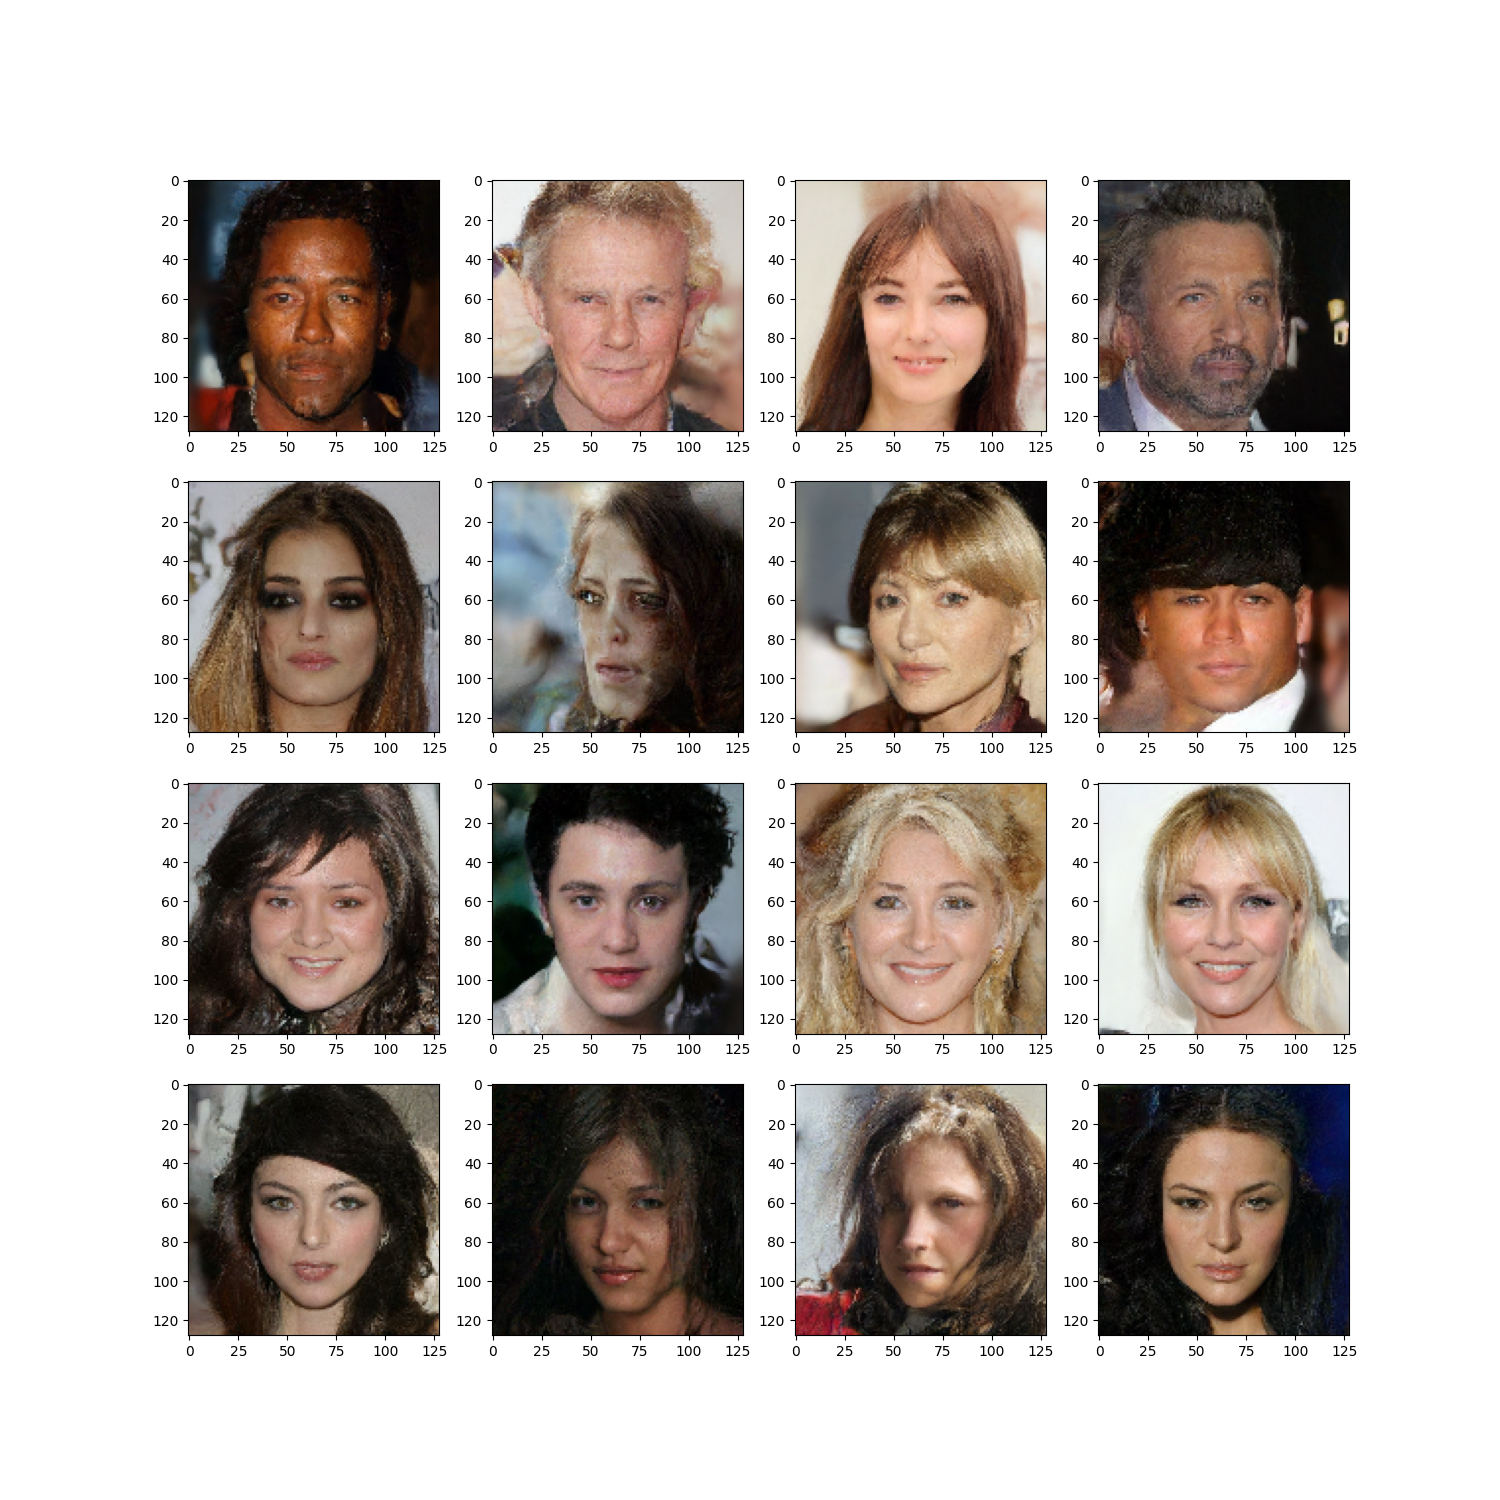
\includegraphics[width=15cm, height = 15cm]{test_batch_DDM_0.png}
    \caption{Images generated by ddm model.}
    \label{fig:diffusion_model}
\end{figure}
\subsection{Relation with VAE}
VAE ELBO per point is defined as follows
\begin{equation}
\label{eq:vae_per_point}
    \mathcal{L}_{\phi, \theta}(\textbf{x}) =  
      \mathbb{E}_{q_{\phi }(\textbf{z}|\textbf{x})}
    \left[ \log p_{\theta }(\textbf{x}| \textbf{z}) +\log p_{\theta}(\textbf{z}) -
   \log q_{\phi }(\textbf{z}|\textbf{x}) \right].
\end{equation}
distributions p and q are defined in the following manner
\begin{gather}
   p_{\theta}(\textbf{z}) = p_{\theta}(\textbf{z}_T)
   \prod^{T}_{t=1} p_{\theta}(\textbf{z}_{t-1}| \textbf{z}_{t}), \\ 
   q_{\phi }(\textbf{z}|\textbf{x})  = q_{\phi }(\textbf{z}_0|\textbf{x}) 
   \prod^{T}_{t=1}  q_{\phi }(\textbf{z}_{t}| \textbf{z}_{t-1}) .
\end{gather}
Substituting into equation (\ref{eq:vae_per_point}) yields
\begin{gather}
    \begin{gathered}
    \mathcal{L}_{\phi, \theta}(\textbf{x}) =  
      \mathbb{E}_{q_{\phi }(\textbf{z}|\textbf{x})}
    \Bigg[ \log p_{\theta }(\textbf{x}| \textbf{z}_0) +
    \log[p_{\theta}(\textbf{z}_T)\prod^{T}_{t=1} p_{\theta}(\textbf{z}_{t-1}| \textbf{z}_{t})]\\ -
   \log [q_{\phi }(\textbf{z}_0|\textbf{x}) 
   \prod^{T}_{t=1}  q_{\phi }(\textbf{z}_{t}| \textbf{z}_{t-1}) ]
   \Bigg] 
       \end{gathered}
       \\
   = \mathbb{E}_{q_{\phi }(\textbf{z}|\textbf{x})} \left[\log p_{\theta }(\textbf{x}| \textbf{z}_0) + \log \frac
   {p_{\theta}(\textbf{z}_T)\prod^{T}_{t=1} p_{\theta}(\textbf{z}_{t-1}| \textbf{z}_{t})}
   {q_{\phi }(\textbf{z}_0|\textbf{x})\prod^{T}_{t=1}  q_{\phi }(\textbf{z}_{t}| \textbf{z}_{t-1})}
   \right] \\
   = \mathbb{E}_{q_{\phi }(\textbf{z}|\textbf{x})} \left[ \log p_{\theta}(\textbf{z}_T) +
   \log \frac
   {p_{\theta }(\textbf{x}| \textbf{z}_0) \prod^{T}_{t=1} p_{\theta}(\textbf{z}_{t-1}| \textbf{z}_{t})} 
   {q_{\phi }(\textbf{z}_0|\textbf{x})\prod^{T}_{t=1}  q_{\phi }(\textbf{z}_{t}| \textbf{z}_{t-1})}
   \right] \\
   = \mathbb{E}_{q_{\phi }(\textbf{z}|\textbf{x})} \left[ \log p_{\theta}(\textbf{z}_T) +
   \log \frac
   { \prod^{T}_{t=0} p_{\theta}(\textbf{z}_{t-1}| \textbf{z}_{t})} 
   {\prod^{T}_{t=0}  q_{\phi }(\textbf{z}_{t}| \textbf{z}_{t-1})}
   \right] \text{,  for } \textbf{z}_{-1} = \textbf{x} \\
   = \label{eq:vae_diff}
   \mathbb{E}_{q_{\phi }(\textbf{z}|\textbf{x})} \left[ \log p_{\theta}(\textbf{z}_T) +
    \sum^T_{t=0}\log \frac
   { p_{\theta}(\textbf{z}_{t-1}| \textbf{z}_{t})} 
   {  q_{\phi }(\textbf{z}_{t}| \textbf{z}_{t-1})}
   \right].
\end{gather}
Above definition of VAE is called structural (or hierarchical \cite{Structured_model}, \cite{Ladder_models} ).
Equation (\ref{eq:vae_diff}) is identical with equation that we obtained during ELBO transformation for diffusion model (\ref{eq:dif_elbo_form}) (with  difference that equation (\ref{eq:vae_diff}) is defined per point), so by applying certain assumptions we could obtain diffusion model. What differs diffusion models and VAEs is explicit definition of distribution q is. That definition gives us increased freedom in ELBO transformation, what ultimately yield better quality of images. Additional difference is interpretation of latent variable $\textbf{z}$. In diffusion models latent variable can be interpreted as noisy image, while in VAEs latent variable does not have interpretation. 
\section{Score models}
\subsection{Introduction}
Score models, in contrary to more common likelihood methods, set as their main objective calculating gradient of density function, that is score function, instead of density function itself. Starting point for score models is relation between normalized and unnormalized density function
\begin{equation}
    p_{\theta}(\textbf{x}) = \frac{f_{\theta}(\textbf{x})}{ Z(\theta)}
    \text{, where } Z(\theta) = \int_{\mathbb{R}^n} f_{\theta}(\textbf{x}) d\textbf{x}.
\end{equation}
$f_{\theta}$ is unnormalized density and $Z(\theta)$ is normalizing factor. Substituting into logarithm gives
\begin{equation}
    \log  p_{\theta}(\textbf{x}) = \log f_{\theta}(\textbf{x}) - \log Z(\theta),
\end{equation}
differentiating both sides with respect to $\textbf{x}$ yields
\begin{equation}
    \nabla_{\textbf{x}} \log  p_{\theta}(\textbf{x}) =  
    \nabla_{\textbf{x}}  \log f_{\theta}(\textbf{x}) -   \nabla_{\textbf{x}}  \log Z(\theta).
\end{equation}
$Z(\theta)$ is constant with respect to $\textbf{x}$, so $\nabla_{\textbf{x}}$, which in turn leads to 
\begin{equation}
     s_{\theta} (\textbf{x}) = \nabla_{\textbf{x}} \log  p_{\theta}(\textbf{x}) =  \nabla_{\textbf{x}}  \log f_{\theta}(\textbf{x}).
\end{equation}
Assume that the true distribution of $\textbf{x}$ is $p^*(\textbf{x})$. Optimization objective is defined as 
\begin{equation}
\label{eq:L}
    \min_{\theta} L(\theta) =  \min_{\theta} \frac{1}{2} \mathbb{E}_{p^*(\textbf{x}) } \Big[ ||\nabla_{\textbf{x}} \log p^*(\textbf{x}) -
    \nabla_{\textbf{x}} \log p_{\theta}(\textbf{x}) ||_2^2 \Big].
\end{equation}
At this point we will prove that if $\theta$ minimizes  $L$ then we get $p^* = p_{\theta}$.
\begin{Twierdzenie}
Suppose that $ P( \omega \in \Omega :  p^*(\textbf{x}) = p_{\theta^*}(\textbf{x})) = 1$ and $f_{\theta} > 0 $ then
\begin{equation}
    L(\theta) = 0 \iff \theta = \theta^*
\end{equation}
\end{Twierdzenie}
Proof \\
\begin{gather}
 L(\theta) = 0 \\
 \implies \nabla_{\textbf{x}} \log p^*(\textbf{x}) =\nabla_{\textbf{x}} \log p_{\theta}(\textbf{x}) \text{ a.s} \\
 \implies  \log p^*(\textbf{x}) =\log p_{\theta}(\textbf{x}) + c \text{ a.s}.
\end{gather}
By the fact that $ p^*$ and $ p_{\theta}$ are density functions c = 0, what gives
\begin{gather}
\log p^*(\textbf{x}) =\log p_{\theta}(\textbf{x}) \text{ a.s}  \\
\implies p^*(\textbf{x}) =  p_{\theta}(\textbf{x}) \text{ a.s}.
\end{gather}
From the assumption that $p^*(\textbf{x}) = p_{\theta^*}(\textbf{x})$ it follows that $\theta = \theta^*$. In order to prove
$\theta = \theta^* \implies  L(\theta) = 0 $ above reasoning needs to be applied in reverse order.
$\blacksquare$
\subsection{Denoising model}
Main problem that is limiting capabilities of our model is space coverage by data points. Said problem is related to manifold hypothesis, which states that multidimensional datasets of real world observations, tend to group together and create manifolds with lower dimension than space in which they exist. Estimating gradient, under assumption manifold hypothesis is true, is prone to errors due to holes in space coverage. 

Method to decrease the problem of space coverage can partially be solved, by introducing additional distribution, which is know and can be sampled from. Image perturbating distribution  will be denoted by $q_{\sigma}( \tilde{\textbf{x}} )$. Optimization objective is to minimize loss function of $ \tilde{\textbf{x} } \sim p^*(\textbf{x})q_{\sigma}( \tilde{\textbf{x}} | \textbf{x})$. In order to find loss function, we start by applying polarization identity on (\ref{eq:L})
\begin{gather}
    \frac{1}{2}\mathbb{E}_{q_{\sigma}( \tilde{\textbf{x}} )} \Big[ ||\nabla_{ \tilde{\textbf{x}}} \log q_{\sigma}( \tilde{\textbf{x} })
    - s_{\theta}(\textbf{x})||_2^2 \Big] \\
    \begin{gathered}
     = \label{eq:sm_loss_nontransfromed} 
     \frac{1}{2}\mathbb{E}_{q_{\sigma}( \tilde{\textbf{x}} )} \Big[ ||\nabla_{\textbf{x}} \log q_{\sigma}( \tilde{\textbf{x} }) ||_2^2 \Big] \\
    + \frac{1}{2}\mathbb{E}_{q_{\sigma}( \tilde{\textbf{x}} ) } \Big[ ||  s_{\theta}(\textbf{x})||_2^2 \Big] \\ 
    -  \mathbb{E}_{q_{\sigma}( \tilde{\textbf{x}} ) } \Big[ < s_{\theta}(\textbf{x}), 
    \nabla_{ \tilde{\textbf{x}}} \log q_{\sigma}( \tilde{\textbf{x}})  >  \Big]. 
    \end{gathered}
\end{gather}
Term $ \mathbb{E}_{q_{\sigma}( \tilde{\textbf{x}} ) } \Big[ ||\nabla_{\textbf{x}} \log q_{\sigma}( \tilde{\textbf{x} }) ||_2^2 \Big]$ does not depend on $\theta$, so it has no influence on optimization process. Because  of that fact we will ignore first term for the time being. 
Term $\mathbb{E}_{q_{\sigma}( \tilde{\textbf{x}} ) } \Big[ < s_{\theta}(\textbf{x}), 
    \nabla_{\textbf{x}} \log q_{\sigma}( \tilde{\textbf{x}})  >  \Big]$, depends on theta so we cannot ignore it. From dot product properties and chain rule for derivative, we obtain
\begin{gather}
    \int q_{\sigma}( \tilde{\textbf{x} })  \Big[ < s_{\theta}(\textbf{x}), 
    \nabla_{\textbf{x}} \log q_{\sigma}( \tilde{\textbf{x}})  >  \Big] d \tilde{\textbf{x} } \\
    =  \int q_{\sigma}( \tilde{\textbf{x} })  \Big[ < s_{\theta}(\tilde{\textbf{x}}), 
   \frac{\partial} {\partial \tilde{\textbf{x}}} \log q_{\sigma}( \tilde{\textbf{x}})  >  \Big] d\tilde{\textbf{x}} \\
   = \int q_{\sigma}( \tilde{\textbf{x} })  \Big[ < s_{\theta}(\textbf{x}), 
    \frac{1}{ q_{\sigma}( \tilde{\textbf{x}})}\frac{\partial} {\partial \tilde{\textbf{x}}} q_{\sigma}( \tilde{\textbf{x}})  >  \Big] d\tilde{\textbf{x}} \\
    =\int  \Big[ < s_{\theta}(\tilde{\textbf{x}}), 
    \frac{\partial} {\partial \tilde{\textbf{x}}} q_{\sigma}( \tilde{\textbf{x}})  >  \Big] d\tilde{\textbf{x}}.
\end{gather}
From properties of marginal distribution ( that is 
$ p(x) = \int p(x,y) dy = \int p(y) p(x|y) dy$ ), it follows that 
\begin{gather}
\int  \Big[ < s_{\theta}(\tilde{\textbf{x}}), 
    \frac{\partial} {\partial \tilde{\textbf{x}}} 
    \int   q_{\sigma}(\textbf{x}, \tilde{\textbf{x}}) d\textbf{x} >  \Big] d\tilde{\textbf{x}} \\
    = \int  \Big[ < s_{\theta}(\tilde{\textbf{x}}), 
    \frac{\partial} {\partial \tilde{\textbf{x}}} 
    \int  p^*(\textbf{x} ) q_{\sigma}(\tilde{\textbf{x}} | \textbf{x}) d\textbf{x} >  \Big] d\tilde{\textbf{x}} \\
    =  \int  \Big[ < s_{\theta}(\tilde{\textbf{x}}), 
    \int p^*(\textbf{x} )  \frac{\partial} {\partial \tilde{\textbf{x}}} q_{\sigma}(\tilde{\textbf{x}} | \textbf{x}) d\textbf{x} >  \Big] d\tilde{\textbf{x}} \\
     =  \int  \Big[ < s_{\theta}(\tilde{\textbf{x}}), 
    \int p^*(\textbf{x} )  
    \frac{ q_{\sigma}(\tilde{\textbf{x}} | \textbf{x})}{ q_{\sigma}(\tilde{\textbf{x}} | \textbf{x})}  \frac{\partial} {\partial \tilde{\textbf{x}}}
    q_{\sigma}(\tilde{\textbf{x}} | \textbf{x}) d\textbf{x} >  \Big] d\tilde{\textbf{x}} \\
      =\label{eq:sm_der_scalar} 
      \int  \Big[ < s_{\theta}(\tilde{\textbf{x}}), 
    \int p^*(\textbf{x} )  q_{\sigma}(\tilde{\textbf{x}} | \textbf{x})  
    \frac{\partial \log q_{\sigma}(\tilde{\textbf{x}} | \textbf{x})} {\partial \tilde{\textbf{x}}}
     d\textbf{x} >  \Big] d\tilde{\textbf{x}}.
\end{gather}
We can note that
\begin{gather}
< s_{\theta}(\tilde{\textbf{x}}), 
    \int p^*(\textbf{x} )  q_{\sigma}(\tilde{\textbf{x}} | \textbf{x})  
    \frac{\partial \log q_{\sigma}(\tilde{\textbf{x}} | \textbf{x})} {\partial \tilde{\textbf{x}}}
     d\textbf{x} >  \\
     =    s_{\theta}(\tilde{\textbf{x}}) ^T \int  p^*(\textbf{x} )  q_{\sigma}(\tilde{\textbf{x}} | \textbf{x})  
    \frac{\partial \log q_{\sigma}(\tilde{\textbf{x}} | \textbf{x})} {\partial \tilde{\textbf{x}}}
     d\textbf{x} \\ 
     =  \int p^*(\textbf{x} )  q_{\sigma}(\tilde{\textbf{x}} | \textbf{x})  
    s_{\theta}(\tilde{\textbf{x}}) ^T  \frac{\partial \log q_{\sigma}(\tilde{\textbf{x}} | \textbf{x})}  {\partial \tilde{\textbf{x}}} d\textbf{x} \\
     = \label{eq:prod_form}
     \int p^*(\textbf{x} )  q_{\sigma}(\tilde{\textbf{x}} | \textbf{x})  
    < s_{\theta}(\tilde{\textbf{x}}),  \frac{\partial \log q_{\sigma}(\tilde{\textbf{x}} | \textbf{x})}  {\partial \tilde{\textbf{x}}} >d\textbf{x}. 
\end{gather}
By substituting (\ref{eq:prod_form}) into (\ref{eq:sm_der_scalar})
\begin{gather}
    \int \int p^*(\textbf{x} )  q_{\sigma}(\tilde{\textbf{x}} | \textbf{x})  
    < s_{\theta}(\tilde{\textbf{x}}),  \frac{\partial \log q_{\sigma}(\tilde{\textbf{x}} | \textbf{x})}  {\partial \tilde{\textbf{x}}} > d\textbf{x}  d\tilde{\textbf{x}} \\
    = \label{eq:2nd_term} 
    \mathbb{E}_{ p^*(\textbf{x} )  q_{\sigma}(\tilde{\textbf{x}} | \textbf{x}) }
    \Big[
    < s_{\theta}(\tilde{\textbf{x}}),  \frac{\partial \log q_{\sigma}(\tilde{\textbf{x}} | \textbf{x})}  {\partial \tilde{\textbf{x}}} > 
    \Big].
\end{gather}
Plugging (\ref{eq:2nd_term}) into (\ref{eq:sm_loss_nontransfromed}) yields
\begin{equation}
\label{eq:sm_part_trans}
    \frac{1}{2} \mathbb{E}_{q_{\sigma}( \tilde{\textbf{x}} ) } \Big[ ||  s_{\theta}(\tilde{\textbf{x}} )||_2^2 \Big]  - 
    \mathbb{E}_{ p^*(\textbf{x} )  q_{\sigma}(\tilde{\textbf{x}} | \textbf{x}) }
    \Big[
    < s_{\theta}(\tilde{\textbf{x}}),  \frac{\partial \log q_{\sigma}(\tilde{\textbf{x}} | \textbf{x})}  {\partial \tilde{\textbf{x}}} > 
    \Big] + C
\end{equation}
where $C = \frac{1}{2}\mathbb{E}_{q_{\sigma} } \Big[ ||\nabla_{\textbf{x}} \log q_{\sigma}( \tilde{\textbf{x} }) ||_2^2 \Big] $. 
Fact that C is independent of $\theta$, makes it possible to set C arbitrarily, with constraint that chosen C cannot depend on $\theta$. Values of function at given point will change, however this does not change values of optimal $\theta$.
Suppose that
$C = \frac{1}{2}\mathbb{E}_{ p^*(\textbf{x} )  q_{\sigma}(\tilde{\textbf{x}} | \textbf{x}) }
\Big[ || \frac{\partial \log q_{\sigma}(\tilde{\textbf{x}} | \textbf{x})}  {\partial \tilde{\textbf{x}}}||_2^2 \Big]$. Substituting into (\ref{eq:sm_part_trans}) gives
\begin{equation}
\label{eq:sm_loss_almost_there}
\begin{gathered}
    \frac{1}{2} \mathbb{E}_{q_{\sigma} } \Big[ ||  s_{\theta}(\tilde{\textbf{x}})||_2^2 \Big] \\
    - \mathbb{E}_{ p^*(\textbf{x} )  q_{\sigma}(\tilde{\textbf{x}} | \textbf{x}) }
    \Big[
    < s_{\theta}(\tilde{\textbf{x}}),  \frac{\partial \log q_{\sigma}(\tilde{\textbf{x}} | \textbf{x})}  {\partial \tilde{\textbf{x}}} > 
    \Big] \\
    + \frac{1}{2}\mathbb{E}_{ p^*(\textbf{x} )  q_{\sigma}(\tilde{\textbf{x}} | \textbf{x}) }
\Big[ || \frac{\partial \log q_{\sigma}(\tilde{\textbf{x}} | \textbf{x})}  {\partial \tilde{\textbf{x}}}||_2^2 \Big].
\end{gathered}
\end{equation}
In order to transform $ \frac{1}{2} \mathbb{E}_{q_{\sigma}( \tilde{\textbf{x}} ) } \Big[ ||  s_{\theta}(\tilde{\textbf{x}})||_2^2 \Big]$, we need make use of trick that conditions $q_{\sigma} $ on $\textbf{x}$ 
\begin{gather}
    \frac{1}{2}\int q_{\sigma}( \tilde{\textbf{x}} )  ||  s_{\theta}(\tilde{\textbf{x}})||_2^2 d\tilde{\textbf{x}} \\ 
    =    \frac{1}{2} \int \int  p^*(\textbf{x})q_{\sigma}( \tilde{\textbf{x}} | \textbf{x} ) 
    ||  s_{\theta}(\tilde{\textbf{x}})||_2^2 d\tilde{\textbf{x}} d \textbf{x} \\
    = \frac{1}{2} \mathbb{E}_{p^*(\textbf{x})q_{\sigma}( \tilde{\textbf{x}} | \textbf{x} )  }
    \Big[ ||  s_{\theta}(\tilde{\textbf{x}})||_2^2 \Big].
\end{gather}
Plugging above result into (\ref{eq:sm_loss_almost_there}) yields
\begin{equation}
\begin{gathered}
     \frac{1}{2} \mathbb{E}_{p^*(\textbf{x})q_{\sigma}( \tilde{\textbf{x}} | \textbf{x} )  }
    \Big[ ||  s_{\theta}(\tilde{\textbf{x}})||_2^2 \Big] \\
    - \mathbb{E}_{ p^*(\textbf{x} )  q_{\sigma}(\tilde{\textbf{x}} | \textbf{x}) }
    \Big[
    < s_{\theta}(\tilde{\textbf{x}}),  \frac{\partial \log q_{\sigma}(\tilde{\textbf{x}} | \textbf{x})}  {\partial \tilde{\textbf{x}}} > 
    \Big] \\
    + \frac{1}{2}\mathbb{E}_{ p^*(\textbf{x} )  q_{\sigma}(\tilde{\textbf{x}} | \textbf{x}) }
\Big[ || \frac{\partial \log q_{\sigma}(\tilde{\textbf{x}} | \textbf{x})}  {\partial \tilde{\textbf{x}}}||_2^2 \Big].
\end{gathered}
\end{equation}
Above function can be folded into
\begin{equation}
\label{eq:sm_loss_fn}
      \frac{1}{2} \mathbb{E}_{p^*(\textbf{x})q_{\sigma}( \tilde{\textbf{x}} | \textbf{x} )  }
    \Big[ ||  s_{\theta}(\tilde{\textbf{x}})  - 
    \frac{\partial \log q_{\sigma}(\tilde{\textbf{x}} | \textbf{x})}  {\partial \tilde{\textbf{x}}} ||_2^2 \Big].
\end{equation}
Equation (\ref{eq:sm_loss_fn}) is our loss function, it is called score denosing function. Optimizing it is equivalent to optimizing (\ref{eq:sm_loss_nontransfromed})
\subsection{Multi-stage  denoising}
\begin{figure}
    \centering
    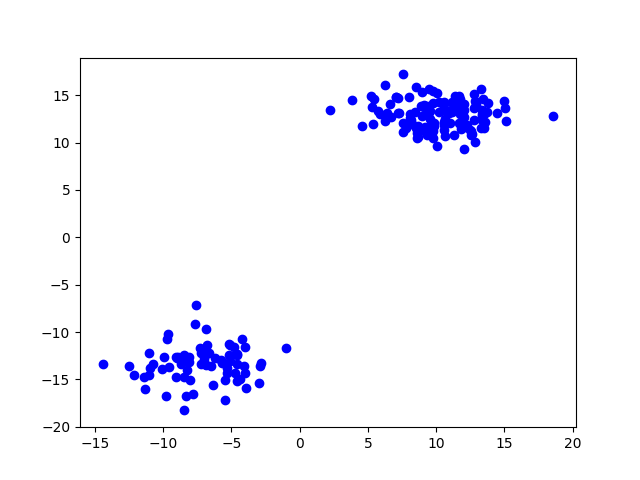
\includegraphics[width = 5cm, height = 5cm]{gauss_przed_szumem.png}
     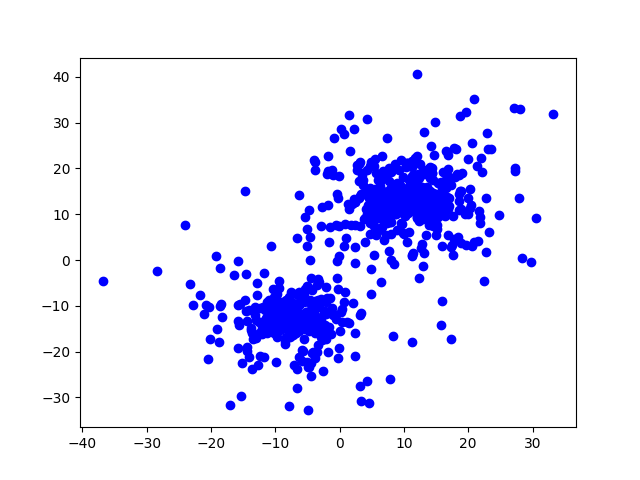
\includegraphics[width = 5cm, height = 5cm]{gauss_po_szumie.png}
    \caption[Filling gaps in dataset with noise.]
    {Left figure shows sample from distribution
    $p(\textbf{x}) = 0.65\mathcal{N}([ 10, 13], [ 9, 2] \mathbf{I} ) + 
    0.35\mathcal{N}([-7, -13], [ 7, 5] \mathbf{I} )$. Right figure presents samples from left figures that are concatenated with samples from distribution  $\mathcal{N}(\textbf{x}, \sigma_t \mathbf{I})$, where  $\textbf{x}$ is single 2d point from left figure and $\sigma_t$ is geometric series such that o $\sigma_1 = 10, q = 0.59948425, T = 10$.}
\label{fig:gauss_comparisson}
\end{figure}
In practice it can turn out that chosen noise level is too strong, what causes quality of generated images to highly deteriorate or too weak to have any influence over training process. Solution to this problem is geometric series of noise levels, such that subsequent values are smaller than previous ones. Thanks to this approach we can have smoother transition between weak noise level that has no influence and strong noise level. Geometric series of noise levels gives us means to control space coverage by data points. Figure \ref{fig:gauss_comparisson} presents example of said approach to filling up empty space in sample space.

Let $q_{\sigma_t}(\tilde{\textbf{x}} | \textbf{x}) = \mathcal{N}(\textbf{x}, \sigma_t \mathbf{I})$. $\sigma_t$ be an element from geometric sequence $\{\sigma_i\}_{i = 1}^L$, that meets the condition
$\frac{\sigma_1}{\sigma_2} = ... = \frac{\sigma_{L-1}}{\sigma_L} > 1$, where $\sigma_L$ is small enough, such that humans cannot see the difference between original image and noisy one.
Sequence $\{\sigma_i\}_{i = 1}^L$  determines how aggressive noise injection process is. From the fact that we have sequence of distributions, in order to let neural network "know" on which noise level it operates, we will condition model 
on $q_{\sigma}$. Additionally $\nabla _{\tilde{\textbf{x}}}  \log q_{\sigma}(\tilde{\textbf{x}} | \textbf{x})
= -\frac{\tilde{\textbf{x}} - \textbf{x}}{ \sigma^2}$ because $q_{\sigma}$ is assumed to be normal distribution. Putting all of our considerations together yields
\begin{equation}
    \ell(\sigma) =  \frac{1}{2} \mathbb{E}_{p^*(\textbf{x})q_{\sigma}( \tilde{\textbf{x}} | \textbf{x} )  }
    \Big[ ||  s_{\theta}(\tilde{\textbf{x}}, \sigma)  +
   \frac{\tilde{\textbf{x}} - \textbf{x}}{ \sigma^2} ||_2^2 \Big].
\end{equation}
From the fact that we have L distributions instead of one, final form of loss function is 
\begin{equation}
    L = \sum_{l=1}^L \lambda(\sigma_l) \ell(\sigma_l),
\end{equation}
where $\lambda(\sigma_l)$ is weight factor set arbitrarily. \\
Calculating loss function L-times is both computationally and memory intensive. To alleviate that, we can use trick from section 3.5 that is
\begin{equation}
    L = \mathbb{E}_{p(l)} \Big[ \lambda(\sigma_l) \ell(\sigma_l) \Big],
\end{equation}
where $l \sim \text{Uniform} \{1, 2, ..., L \}$.
\begin{algorithm} [H]
\caption{Training loop for gaussian score model}\label{alg:cap}
\begin{algorithmic}
    \While{$\theta$ divergent}
    \State $\textbf{x} \sim p^*(\textbf{x})$
    \State $l \sim \text{Uniform}\{1, 2, ... , L\}$.
    \State $\bm{\epsilon} \sim \mathcal{N}(0, \mathbf{I})$.
    \State $ \tilde{\textbf{x}} = \textbf{x} + \sigma_l \bm{\epsilon}$
    \State $L \gets \frac{1}{N} \sum_{n=1}^N  \lambda(\sigma_l)
    ||  s_{\theta}(\tilde{\textbf{x}}, \sigma_l)  +
   \frac{\tilde{\textbf{x}} - \textbf{x}}{ \sigma_l^2} ||_2^2 $
    \State $\theta_{k+1} \gets \theta_{k} - \eta \nabla_{\theta}L$
    \EndWhile
\end{algorithmic}
\end{algorithm}
From properties of gaussian distribution it follows that $x \sim \mathcal{N}(a, b^2)$ i  $\epsilon \sim \mathcal{N}(0, 1)$ to $x = a + b\epsilon$ and $ \epsilon = \frac{x- a}{b}$. Considering that $\tilde{\textbf{x}} \sim \mathcal{N}(\textbf{x}, \sigma_t \mathbf{I})$ loss function can be written as
\begin{gather}
    \min ||  s_{\theta}(\tilde{\textbf{x}}, \sigma)  + \frac{\tilde{\textbf{x}} - \textbf{x}}{ \sigma_l^2} ||_2^2 \\
    = min ||  s_{\theta}(\tilde{\textbf{x}}, \sigma)  + \frac{1}{\sigma_l} \frac{\tilde{\textbf{x}} - \textbf{x}}{ \sigma_l} ||_2^2 \\
    \iff \min \Big|\Big|  s_{\theta}(\tilde{\textbf{x}}, \sigma)  + \frac{ \bm{\epsilon} }{ \sigma_l} \Big|\Big|_2^2 \\
    \iff \min ||  s_{\theta}(\tilde{\textbf{x}}, \sigma_l) \sigma_l + \bm{\epsilon} ||_2^2
\end{gather}

\subsection{Sampling}
Suppose we have trained model  $ s_{\theta}(\tilde{\textbf{x}}, \sigma)$, however we cannot sample gradient of density function. In \cite{score_model} authors proposed algorithm for sampling using gradient of a density function, based on Langevin dynamics. 

\begin{algorithm} [H]
\caption{Sampling score model}\label{alg:cap}
\begin{algorithmic}

\State $\textbf{x}_0 \sim p_{prior}(\textbf{x}_0)$
\For{\text{i in 1:L}}
    \State $\alpha_i \gets  \epsilon$ $\frac{ \sigma_i^2 }{\sigma_L^2 }$
    \For{\text{t in 1:T}}
        \State $\textbf{z}_t \sim \mathcal{N}(0, \mathbf{I})$
       \State $\textbf{x}_t \gets \textbf{x}_{t -1} + \frac{\alpha_i}{2} s(\textbf{x}_{t -1}, \sigma_i ) + \sqrt{\alpha_i}\textbf{z}_t$
    \EndFor
    \State $\textbf{x}_0 \gets \textbf{x}_T$
\EndFor
\State \textbf{return} $\textbf{x}_0$
\end{algorithmic}
\end{algorithm}

\subsection{Implementation}

\begin{figure}
    \centering
\hspace*{-2cm}  
    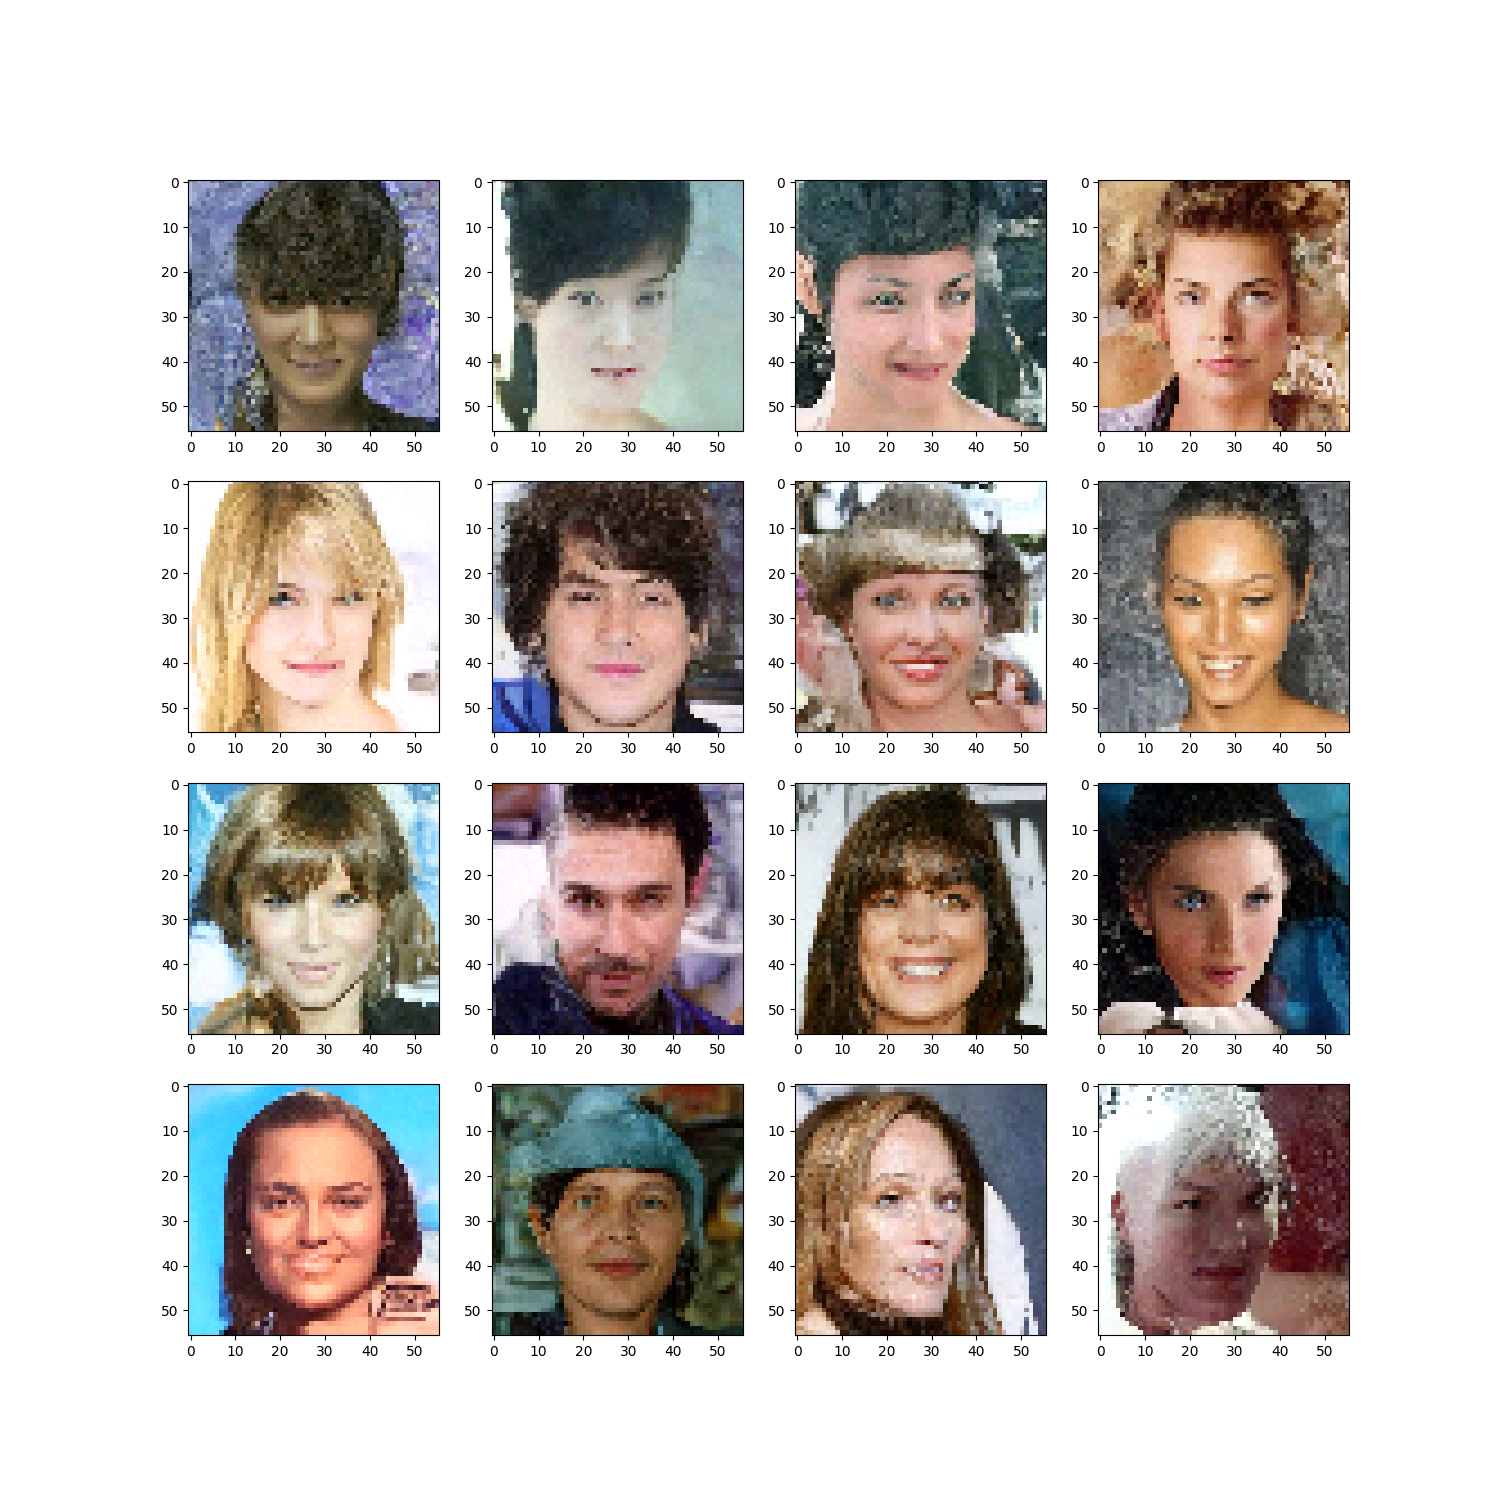
\includegraphics[width = 16cm, height = 16cm]{score_model_500.png}
    \caption{Sample generated by score model.}
    \label{fig:score_example}
\end{figure}
Images were scaled down to resolution 56x56 and RGB channels to the interval [0,1].
I set L = 30,  $\lambda(\sigma_l) = 1$,  $\sigma_1 = 30,  q =  0.7395,  a_{30} = 0.01 $ in contrary to recommendations from \cite{improved_score} which was dictated by limited computational resources. Neural network architecture was refine-net with around 10 million parameters. Model was trained for 500 iteration over  Celeba-HQ \cite{celeba_hq} dataset.

Samples generated by the trained model is shown in figure \ref{fig:score_example}. The realization that reader may have, is fact that both image resolution and model size is much smaller compared to diffusion model. It stems from the fact that refinet architecture turned out to be much more computationally expensive than architecture used in previous chapter. Regarding image quality, we can see that model, despite occasional artefacts, is able to keep structure of human face at level, that person looking at the image, can classify as  a human face. Artifacts can be partially explained by much stronger down scaling of resolution to 56x56.
\subsection{Relation to diffusion models}

Suppose that $\{ \sigma_i \}_{i=1}^T$ is growing sequence, such that $0 < \sigma_k< 1$. Let
\begin{equation}
q_{\sigma}( \tilde{\textbf{x}}_t | \tilde{\textbf{x}}_{t-1}) =
\mathcal{N}( \sqrt{1 - \sigma_t}  \tilde{\textbf{x}}_{t-1}, \sigma_t \mathbf{I} )
\end{equation}
be a Markov chain.
Thus, we obtain (proof is in section 3.3)
\begin{equation}
q_{\sigma}( \tilde{\textbf{x}} | \textbf{x} ) =
\mathcal{N}( \sqrt{\overline{\alpha}_{t}} \textbf{x} , (1 - \overline{\alpha}_{t}) \mathbf{I} ).
\end{equation}
where $ \overline{\alpha}_{t} = \prod_{i=1}^t (1 - \sigma_i)$.
Let our model be defined as 
\begin{equation}
s_{\theta}( \tilde{\textbf{x}}, \sigma_t ) = \frac{-1}{ \sqrt{1 - \overline{\alpha}_{t}} } g_{\theta}(\tilde{\textbf{x}}, \sigma_t ).
\end{equation}
Weight factor will be set to 
\begin{equation}
    \lambda(\sigma_t) = 2( 1 - \overline{\alpha}_{t}).
\end{equation}
Let $t \sim \text{Uniform} \{1, 2, ..., L \}$, then loss function will take following form
\begin{gather}
    \mathbb{E}_{p(t)}
    \mathbb{E}_{p^*(\textbf{x})q_{\sigma}( \tilde{\textbf{x}} | \textbf{x} )  }
    \Big[  (1 - \overline{\alpha}_{t}) || \frac{-1}{ \sqrt{1 - \overline{\alpha}_{t}} } g_{\theta}(\tilde{\textbf{x}}, \sigma_t )  +
   \frac{\tilde{\textbf{x}} -\sqrt{\overline{\alpha}_{t}} \textbf{x} }
   { 1 - \overline{\alpha}_{t}} ||_2^2 \Big] \\
   = \mathbb{E}_{p(t)}
    \mathbb{E}_{p^*(\textbf{x})q_{\sigma}( \tilde{\textbf{x}} | \textbf{x} )  }
    \Big[ || g_{\theta}(\tilde{\textbf{x}}, \sigma_t )  -
   \frac{\tilde{\textbf{x}} -\sqrt{\overline{\alpha}_{t}} \textbf{x} }
   { \sqrt{1 - \overline{\alpha}_{t}} } ||_2^2 \Big].
\end{gather}
We can note that:
\begin{enumerate}
    \item   $\frac{\tilde{\textbf{x}} -\sqrt{\overline{\alpha}_{t}} \textbf{x} }
   { \sqrt{1 - \overline{\alpha}_{t}} } = \bm{\epsilon} \sim N(0, \mathbf{I})$
   because $\tilde{\textbf{x}} \sim  \mathcal{N}( \sqrt{\overline{\alpha}_{t}} \textbf{x} , (1 - \overline{\alpha}_{t}) \mathbf{I} ) $,
   \item $ g_{\theta}(\tilde{\textbf{x}}, \sigma_t ) =
   g_{\theta}(\sqrt{\overline{\alpha}_{t}} \textbf{x} +  \sqrt{1 - \overline{\alpha}_{t}} \bm{\epsilon}, \sigma_t ) $.
\end{enumerate}
From point 1 it follows that 
$\tilde{\textbf{x}} = y(\textbf{x}, \bm{\epsilon}) = \sqrt{\overline{\alpha}_{t}} \textbf{x} +  \sqrt{1 - \overline{\alpha}_{t}} \bm{\epsilon_t}$, so by applying reparametrization trick we obtain 
\begin{equation}
\label{eq:sm_loss_diff}
    \mathbb{E}_{p(t)}
    \mathbb{E}_{p^*(\textbf{x})p(\bm{\epsilon}) }
    \Big[ || g_{\theta}(\sqrt{\overline{\alpha}_{t}} \textbf{x} +  \sqrt{1 - \overline{\alpha}_{t}} \bm{\epsilon}, \sigma_t ) - \bm{\epsilon}||_2^2 \Big].
\end{equation}
Loss function in form (\ref{eq:sm_loss_diff}) is equivalent to loss function of diffusion model (\ref{eq:ddm_loss_real}). This leads us to the conclusion, that diffusion models are different way to describe certain group of problems, that share common traits.
\section{Data perturbation as stochastic process }
\subsection{Stochastic process construction}
As it turns out, data perturbation that we used in previous sections, can be defined in terms of stochastic processes. To be precise, role of the perturbation process is to transform data sampled from distribution $p_{\text{data}}(\hat{\textbf{x} } )$ into data that has distribution $p_{\text{prior}}(\hat{\textbf{x} } )$, where $p_{\text{prior}}(\hat{\textbf{x} } )$ is known distribution, that can be sampled. Let $\{ \textbf{x}_t\}_{t=0}^T$ be a stochastic process, which for $ \hat{\textbf{x} } \sim p_{\text{data}}( \hat{\textbf{x} } )$ meets the following criteria:

\begin{enumerate}
    \item $ P( \textbf{x}_0  =  \hat{\textbf{x} } ) = 1$,
    \item $\textbf{x}_T \sim  p_{\text{prior}}(\hat{\textbf{x} } )$.
\end{enumerate}
It is worth to note that $\mathbb{E}[\textbf{x}_0] =  \hat{\textbf{x} }$ and $\text{Var}[\textbf{x}_0] = 0$, those properties will be important further into this section.

Stochastic process can be defined in terms of it's changes through time. In order to do so, we will use stochastic differential equation. Let $ \textbf{f}: \mathbb{R}^{n + 1} \to \mathbb{R}^n $ and $ \textbf{G}: \mathbb{R}^{n + 1} \to \mathbb{R}^{n \times n} $, then stochastic differential equation that describes distribution of stochastic process $\{ \textbf{x}_t\}_{t=0}^T$ at time t, has the following form
\begin{equation}
    d\textbf{x}_t =  \textbf{f}(\textbf{x}_t, t) dt +  \textbf{G}(\textbf{x}_t, t)d\textbf{w}.
\end{equation}
Let $t_0 \leq s \leq t \leq T$, by $p_{s,t}(\textbf{x}_t | \textbf{x}_s)$ we will denote perturbation kernel of random variable $\textbf{x}_t$. The main focus of ours is distribution  $p_{0,t}(\textbf{x}_t | \textbf{x}_0)$, as it is used to sample perturbated data during neural network training process. From that fact it follows, that distribution 
$p_{0,t}(\textbf{x}_t | \textbf{x}_0)$  must have form, that allows it to be sampled.

To meet that condition, function $\textbf{f}(\textbf{x}_t, t)$ will be limited to the set of affine functions and we will drop conditioning of function $\textbf{G}(\textbf{x}_t, t)$ on $\textbf{x}_t$. Those assumptions will make it much easier to find distribution $p_{0,t}(\textbf{x}_t | \textbf{x}_0)$ explicitly. In general it is possible to use Fokker-Planck equation to find probability density function, but considering multidimensionality of our process and complexity of partial differential equations, solving said equation might be hard or even impossible.

\subsection{Stochastic process with reverse time}
In order to be able to create samples using neural networks, we must be able to obtain 
$\textbf{x}_0$ given $\textbf{x}_T$. The solution to this issue is the following theorem proposed and proven in  \cite{reverse_time_SDE}.
\begin{Twierdzenie}[reverse-time stochastic process]
Let $\{ \textbf{x}_t\}_{t=0}^T$ be a stochastic process, described by stochastic differential equation
$d\textbf{x}_t =  \textbf{f}(\textbf{x}_t, t) dt +  \textbf{G}(\textbf{x}_t, t)d\textbf{w}$. Suppose that $ \textbf{f}: \mathbb{R}^{n + 1} \to \mathbb{R}^n $ and $ \textbf{G}: \mathbb{R}^{n + 1} \to \mathbb{R}^{n \times n} $ guarantee existence of the probability density function $p(\textbf{x}_t, t)$ for$t_0 \leq t \leq T$,
which is smooth and is unique solution to it's Fokker-Planck equation (Kolmogorov forward equation). Let $\textbf{w}_t = [w_t^{(1)}, ... , w_t^{(n)}]$ denote vector of the Wiener processes  and $\overline{\textbf{w}_t}$ denote vector of the reverse processes, such that   $\overline{\textbf{w}_{t_0}} = 0 $ and
\begin{equation}
    d\overline{w_t}^{(i)} =
    dw_t^{(i)} + \frac{1}{p(\textbf{x}_t, t)}  \sum_{j} \frac{\partial}{\partial \textbf{x}_t^{(j)}} \Big[p(\textbf{x}_t , t)  g^{(j,i)}(\textbf{x}_t , t) \Big]dt.
\end{equation}
Suppose that Fokker-Planck equation of joint process $(\textbf{x}_t,\textbf{w}_t )$ has smooth and unique solution for $p(\textbf{x}_t,\overline{\textbf{w}}_t, t )$ when $t > t_0$ and for 
$p(\textbf{x}_t,\overline{\textbf{w}}_t, t | \overline{\textbf{w}}_s, s)$, when $t > s \geq t_0$. Then
\begin{enumerate}
    \item $\textbf{x}_t$ and $\overline{\textbf{w}}_t - \overline{\textbf{w}}_s$ are independent for $t \geq s \geq t_0$.
    \item For minimal $\sigma$-algebra $A_t$ with respect to which $\textbf{x}_s$ and  $\overline{\textbf{w}}_s$ for $s \geq t $  are measurable, following conditions holds $\mathbb{E}[\overline{\textbf{w}}_t | A_{t+s}] = \overline{\textbf{w}}_{t+s}$ i \\ $\mathbb{E}[(\overline{\textbf{w}}_t -  \overline{\textbf{w}}_{t+s})(\overline{\textbf{w}}_t -  \overline{\textbf{w}}_{t+s})^T| A_{t+s}] = s\mathbf{I}$.
    \item A reverse time model is defined by 
    \begin{equation}
        d \textbf{x}_t = \overline{\textbf{f}} (\textbf{x}_t , t) dt + \textbf{G} (\textbf{x}_t , t)
        d \overline{\textbf{w}} _t,
    \end{equation}
    where 
    \begin{equation}
    \begin{gathered}
        \overline{f}^{(i)}(\textbf{x}_t , t) \\
        =  f^{(i)}(\textbf{x}_t , t) - \frac{1}{p(\textbf{x}_t , t)} 
        \sum_{j, k} \frac{\partial}{\partial x_t^{(j)}} \Big[p(\textbf{x}_t , t)
        g^{(i,k)}(\textbf{x}_t , t)  g^{(j,k)}(\textbf{x}_t , t) \Big].
    \end{gathered}
    \end{equation}
\end{enumerate}
\end{Twierdzenie}
Let $ \overline{\textbf{f}}(\textbf{x}_t , t) = [ \overline{f}^{(1)}(\textbf{x}_t , t), ... ,  \overline{f}^{(n)}(\textbf{x}_t , t)]$. $ \overline{\textbf{f}}(\textbf{x}_t , t)$ can be expressed in matrix form as
\begin{equation}
\label{eq:f_hat}
 \overline{\textbf{f}}(\textbf{x}_t , t) =
    \textbf{f}(\textbf{x}_t , t) - \frac{1}{p(\textbf{x}_t , t)}\frac{\partial}{\partial \textbf{x}} \Big[ \textbf{G}(\textbf{x}_t, t) \textbf{G}(\textbf{x}_t, t) ^T p(\textbf{x}_t , t) \Big].
\end{equation}

In order to find derivative in equation (\ref{eq:f_hat}), we will start by writing matrix multiplication in summation form. Then by applying rules of differentiation we obtain 
\begin{gather} 
        \sum_{j, k} \frac{\partial}{\partial x_t^{(j)}} \Big[p(\textbf{x}_t , t)
        g^{(i,k)}(\textbf{x}_t , t)  g^{(j,k)}(\textbf{x}_t , t) \Big] \\
        = \sum_{j} \sum_k  \frac{\partial}{\partial x_t^{(j)}} \Big[p(\textbf{x}_t , t)
        g^{(i,k)}(\textbf{x}_t , t)  g^{(j,k)}(\textbf{x}_t , t) \Big] \\
         \begin{gathered}
        =\sum_{j} \sum_k \Big(  \frac{\partial p(\textbf{x}_t , t)}{\partial x_t^{(j)}} \Big[
        g^{(i,k)}(\textbf{x}_t , t)  g^{(j,k)}(\textbf{x}_t , t) \Big]  \\
        +  p(\textbf{x}_t , t) \sum_{j} \sum_k \frac{\partial}{\partial x_t^{(j)}} \Big[
        g^{(i,k)}(\textbf{x}_t , t)  g^{(j,k)}(\textbf{x}_t , t) \Big] \Big)
        \end{gathered}\\
        \begin{gathered} \label{eq:grad_sde} = 
        \sum_{j}  \frac{\partial p(\textbf{x}_t , t)}{\partial x_t^{(j)}}  \sum_k \Big[
        g^{(i,k)}(\textbf{x}_t , t)  g^{(j,k)}(\textbf{x}_t , t) \Big]  \\
          + p(\textbf{x}_t , t) \sum_{j}\frac{\partial}{\partial x_t^{(j)}}  \sum_k \Big[
        g^{(i,k)}(\textbf{x}_t , t)  g^{(j,k)}(\textbf{x}_t , t) \Big].
               \end{gathered}
\end{gather}
Equation (\ref{eq:grad_sde}) can be expressed in matrix notation in following manner
( to keep notation more compact, suppose that for square matrix \textbf{G} with n elements, we define operation $\nabla \cdot \textbf{G}(\textbf{x}_t, t) = [\nabla \cdot \textbf{g}^1(\textbf{x}_t, t), ... ,\nabla \cdot \textbf{g}^n(\textbf{x}_t, t) ]$, where $g^{(k)}$ is k-th row)
\begin{gather}
    \frac{\partial}{\partial \textbf{x}} \Big[ \textbf{G}(\textbf{x}_t, t) \textbf{G}(\textbf{x}_t, t) ^T p(\textbf{x}_t , t) \Big] \\
    = \label{eq:sde_grad_G}
    \Big[ \textbf{G}(\textbf{x}_t, t) \textbf{G}(\textbf{x}_t, t) ^T \Big]
    \nabla_{\textbf{x}} p(\textbf{x}_t , t)
    +
    p(\textbf{x}_t , t) \nabla_{\textbf{x}} \cdot  \Big[ \textbf{G}(\textbf{x}_t, t) \textbf{G}(\textbf{x}_t, t) ^T \Big]
\end{gather}
Substituting (\ref{eq:sde_grad_G}) into (\ref{eq:f_hat}) yields
\begin{gather}
   \overline{\textbf{f}}(\textbf{x}_t , t) 
     =\textbf{f}(\textbf{x}_t , t) - \frac{1}{p(\textbf{x}_t , t)}\frac{\partial}{\partial \textbf{x}} \Big[ \textbf{G}(\textbf{x}_t, t) \textbf{G}(\textbf{x}_t, t) ^T p(\textbf{x}_t , t) \Big] \\
     =  \textbf{f}(\textbf{x}_t , t) - \frac{1}{p(\textbf{x}_t , t)} \Big( \Big[ \textbf{G}(\textbf{x}_t, t) \textbf{G}(\textbf{x}_t, t) ^T \Big]
    \frac{\partial p(\textbf{x}_t , t)}{\partial \textbf{x}} ^T 
    +
    p(\textbf{x}_t , t) \nabla_{\textbf{x}} \cdot  \Big[ \textbf{G}(\textbf{x}_t, t) \textbf{G}(\textbf{x}_t, t) ^T \Big] \Big)\\
    = \textbf{f}(\textbf{x}_t , t) - \Big[ \textbf{G}(\textbf{x}_t, t) \textbf{G}(\textbf{x}_t, t) ^T \Big]
    \frac{1}{p(\textbf{x}_t , t)} 
    \frac{\partial p(\textbf{x}_t , t)}{\partial \textbf{x}} ^T 
    - \nabla_{\textbf{x}} \cdot  \Big[ \textbf{G}(\textbf{x}_t, t) \textbf{G}(\textbf{x}_t, t) ^T \Big] \\
    = \textbf{f}(\textbf{x}_t , t) - \Big[ \textbf{G}(\textbf{x}_t, t) \textbf{G}(\textbf{x}_t, t) ^T \Big] 
    \nabla_{\textbf{x}} \log p(\textbf{x}_t , t)
    - \nabla_{\textbf{x}} \cdot  \Big[ \textbf{G}(\textbf{x}_t, t) \textbf{G}(\textbf{x}_t, t) ^T \Big] 
\end{gather}
Plugging above result into reverse time stochastic differential equation gives
\begin{equation}
\label{eq:rv_time:sde}
\begin{gathered}
     d \textbf{x}_t = \Big(
     \textbf{f}(\textbf{x}_t , t) - \Big[ \textbf{G}(\textbf{x}_t, t) \textbf{G}(\textbf{x}_t, t) ^T \Big] 
    \nabla_{\textbf{x}} \log p(\textbf{x}_t , t)\\
    - \nabla_{\textbf{x}} \cdot  \Big[ \textbf{G}(\textbf{x}_t, t) \textbf{G}(\textbf{x}_t, t) ^T \Big] \Big) dt + \textbf{G} (\textbf{x}_t , t)
        d \overline{\textbf{w}} _t
\end{gathered}
\end{equation}
We will not solve equation (\ref{eq:rv_time:sde}) explicitly, instead we will use numerical algorithms such as Euler-Murayama method or predictor-corretor
\subsection{Construction of stochastic differential equations}
\subsubsection{Variance Exploding}
Let $\{ \textbf{x}_i \}_{i=0}^T$ denote stochastic process, such that $p_{\sigma_i}(\textbf{x}_i | \textbf{x}) = \mathcal{N}(\textbf{x}, \sigma_i^2 \mathbf{I})$, $\sigma_t$ is element from N-element sequence $\{ \sigma_i\}_{i=0}^T$ and $\sigma_0 = 0$. Then
\begin{equation}
    p_{\sigma_i}(\textbf{x}_i | \textbf{x}_{i-1}) = \mathcal{N}(\textbf{x}_{i-1},
    (\sigma_i^2 - \sigma_{i-1}^2) \mathbf{I}).
\end{equation}
Proof \\ 
Let $\textbf{x}_i \sim  p_{\sigma_i}(\textbf{x}_i | \textbf{x}_{i-1})$, for $\bm{\epsilon_{i}} \sim N(0, \mathbf{I}) $ we obtain
\begin{equation} \label{eq:ve_dics}
        \textbf{x}_i = \textbf{x}_{i-1} +  \sqrt{\sigma_i^2 - \sigma_{i-1}^2} \bm{\epsilon}_{i}.
\end{equation}
$\textbf{x}_{i-1}$ can be decomposed into 
\begin{equation}
\label{eq:variable}
        \textbf{x}_i = \textbf{x}_{i-2} + \sqrt{\sigma_{i-1}^2 - \sigma_{i-2}^2} \bm{\epsilon}_{i-2} +  \sqrt{\sigma_i^2 - \sigma_{i-1}^2} \bm{\epsilon}_{i}.
\end{equation}
In equation (\ref{eq:variable}) we can apply substitution  $\textbf{X} = \textbf{x}_{i-2} + \sqrt{\sigma_{i-1}^2 - \sigma_{i-2}^2} \bm{\epsilon}_{i-2}$ and $\textbf{Y} = 0 + \sqrt{\sigma_i^2 - \sigma_{i-1}^2} \bm{\epsilon}_{i}$. From this substitution it follows that
\begin{enumerate}
    \item $\textbf{X} \sim \mathcal{N}( \textbf{x}_{i-2},(\sigma_{i-1}^2 - \sigma_{i-2}^2)\mathbf{I}) $,
    \item $\textbf{Y} \sim \mathcal{N}( 0,(\sigma_{i}^2 - \sigma_{i-1}^2)\mathbf{I}) $,
    \item $ \textbf{x}_i = \textbf{X} + \textbf{Y}$.
\end{enumerate}
Based on theorem \ref{gaussian_sum_dist} we obtain 
\begin{equation}
    \textbf{x}_i \sim \mathcal{N} ( \textbf{x}_{i-2},(\sigma_{i}^2  - \sigma_{i-2}^2)\mathbf{I} ).
\end{equation}
We can apply above reasoning until we get
\begin{equation}
    \textbf{x}_i \sim \mathcal{N} ( \textbf{x}_{i-2},(\sigma_{i}^2  - \sigma_{i-2}^2 + \sigma_{i-2}^2  - ... + \sigma_0^2)\mathbf{I} ),
\end{equation}
what can be simplified into
\begin{equation}
      \textbf{x}_i \sim \mathcal{N} ( \textbf{x},\sigma_{i}^2  \mathbf{I} ),
\end{equation}
what concludes the proof.$\blacksquare$ \\
Let  $\{ \hat{\textbf{x}}_t \}_{t=0}^1$ be a stochastic process, where $t \in [0,1]$. Suppose that  
  $\hat{\sigma}:[0, 1] \to \mathbb{R}$, $\hat{\textbf{x}}_{\frac{i}{T}} =\textbf{x}_{i}$ , 
  $\hat{\sigma}(\frac{i}{T})  = \sigma__{i}$,  $\Delta t = \frac{1}{T}$ when  $t \in \{0, \frac{1}{T}, ..., \frac{T-1}{T}\}$,
then
\begin{gather}
     \hat{\textbf{x}}_{t + \Delta t} = \hat{\textbf{x}}_{t} + 
     \sqrt{\hat{\sigma}(t + \Delta t)^2 - \hat{\sigma}(t)^2} \bm{\epsilon}_{t + \Delta t}\\
     = \hat{\textbf{x}}_{t} + \sqrt{\frac{\hat{\sigma}(t + \Delta t)^2 - \hat{\sigma}(t)^2 }{\Delta t}}
     \sqrt{\Delta t} \bm{\epsilon}_{t + \Delta t}.
\end{gather}
As $T \to \infty$ i $\Delta t \to 0$ we obtain
\begin{equation}
\label{eq:Var_Exp}
    d \hat{\textbf{x}} = \sqrt{ \frac{d [ \hat{\sigma}(t)^2]}{dt} } d \textbf{w}.
\end{equation}
Equation (\ref{eq:Var_Exp}) is called Variance Exploding (VE). In order to find parameters of distribution $p_{0,t}$ we will make use of the following property ( \cite{Särkkä_Solin_2019} section 5.5 page 70)
\begin{equation} \label{eq:sarkka}
    \begin{cases}
      \frac{d \mathbb{E}[\textbf{x}_t] }{dt} = \mathbb{E}[\textbf{f}(\textbf{x}_t, t) ]\\
       \frac{d Cov[\textbf{x}_t] }{dt} = \mathbb{E}\Big[\textbf{f}(\textbf{x}_t, t) (\textbf{x}_t -\mathbb{E}[\textbf{x}_t]  )^T \Big] + \mathbb{E} \Big[ (\textbf{x}_t -\mathbb{E}[\textbf{x}_t]  )\textbf{f}(\textbf{x}_t, t)^T \Big] 
       + \mathbb{E} \Big[ \textbf{G}(\textbf{x}_t, t)  \textbf{Q} \textbf{G}(\textbf{x}_t, t)^T \Big],
    \end{cases}\,
\end{equation}
where $\textbf{Q} $ is diffusion matrix. Unless explicitly stated, we assume that
$\textbf{Q} = \mathbf{I}$.\\
For VE  system of equations is defined as 
\begin{equation}
    \begin{cases}
      \frac{d \mathbb{E}[\textbf{x}_t] }{dt} = 0\\
       \frac{d Cov[\textbf{x}_t] }{dt} =  
       \mathbb{E} \Big[ \frac{d [ \hat{\sigma}(t)^2]}{dt}\Big] 
    \end{cases},
\end{equation}

\begin{equation}
    \begin{cases}
      \mathbb{E}[\textbf{x}_t]  = C_0\\
       Cov[\textbf{x}_t] =   \hat{\sigma}(t)^2 + D_0
    \end{cases}.
\end{equation}
From initial conditions   $\mathbb{E}[\textbf{x}_0] =  \hat{\textbf{x} }$ and $\text{Var}[\textbf{x}_0] = 0$ it follows that
\begin{equation}
    \begin{cases}
\mathbb{E}[\textbf{x}_t] = \hat{\textbf{x} } \\
Cov[\textbf{x}_t] = \hat{\sigma}^2(t) -\hat{\sigma}^2(0) 
    \end{cases}.
\end{equation}
Above system of equations defined distribution $p_{0,t}(\textbf{x}_t |\textbf{x}_0 ) = \mathcal{N}(\textbf{x}_0, [\hat{\sigma}^2(t) -\hat{\sigma}^2(0) ]\mathbf{I})$.
\subsubsection{Variance Preserving}
Let $\{ \textbf{x}_i \}$ be a Markov chain such that
\begin{equation}
    \textbf{x}_i =   \sqrt{1 - \beta_i }\textbf{x}_{i-1} + \sqrt{\beta_i} \bm{\epsilon}_{i}, \
    \bm{\epsilon}_{i} \sim \mathcal{N}(0, \mathbf{I}).
\end{equation}
Suppose that $ \{ \tilde{\beta} = T\beta_i \}_{i=1}^T$, what leads to
\begin{equation}
    \textbf{x}_i =   \sqrt{1 - \frac{\tilde{\beta}_i}{T} }\textbf{x}_{i-1} + 
    \sqrt{\frac{\tilde{\beta}_i}{T}} \bm{\epsilon}_{i}, \
    \bm{\epsilon}_{i} \sim \mathcal{N}(0, \mathbf{I}).
\end{equation}
Let  $\{ \hat{\textbf{x}}_t \}_{t=0}^1$ be a stochastic processn where $t \in [0,1]$,
$\hat{\beta}:[0, 1] \to \mathbb{R} $ is a function, $ \hat{\textbf{x}}_{\frac{i}{T}} =\textbf{x}_{i}$, $ \hat{\beta}(\frac{i}{T})  = \tilde{\beta}_i$, $\Delta t = \frac{1}{T}$, $t \in \{0, \frac{1}{T}, ...,   \frac{T-1}{T}\}$, then 
\begin{gather}
    \hat{\textbf{x}}_{t + \Delta t} = \sqrt{1 - \hat{\beta}(t + \Delta t) \Delta t  } \hat{\textbf{x}}_{t} + 
     \sqrt{\hat{\beta}(t + \Delta t) \Delta t  } \bm{\epsilon}_{t + \Delta t}.
\end{gather}
From the fact that near 0 we have $\sqrt{1 - x } \approx 1 - \frac{x}{2}$ it follows that
\begin{equation}
      \hat{\textbf{x}}_{t + \Delta t} = \hat{\textbf{x}}_{t} - \frac{1}{2}\hat{\beta}(t + \Delta t) \Delta t \hat{\beta}{\textbf{x}}_{t} + 
     \sqrt{\beta(t + \Delta t)} \sqrt{\Delta t} \bm{\epsilon}_{t + \Delta t}.
\end{equation}
As $T \to \infty$ i $\Delta t \to 0$
\begin{equation}
\label{eq:VP_eq}
    d  \hat{\textbf{x}}_{t} = - \frac{1}{2}\hat{\beta}(t)  \hat{\textbf{x}}_{t} dt + \sqrt{\hat{\beta}(t)} d \textbf{w}.
\end{equation}
Equation (\ref{eq:VP_eq}) is called Variance Preserving (VP).
From property (\ref{eq:sarkka}) we obtain
\begin{equation}
    p_{0,t}(\textbf{x}_t |\textbf{x}_0 ) =
    \mathcal{N}\left(\textbf{x}_0 \text{e}^{-\frac{1}{2}\int_0^t  \hat{\beta}(s)ds},
    \mathbf{I} - \mathbf{I}\text{e}^{\int_0^t  \hat{\beta}(s)ds}\right).
\end{equation}


\subsection{Training}
Optimization objective is almost the same as in previous section. The difference stems from the fact that $t$ has continuous distribution, that is $t \sim \text{Uniform} [0, 1]$.

\begin{equation}
    \min_{\theta} \mathbb{E}_{p(t)}\frac{1}{2} \lambda(t) \mathbb{E}_{p^*(\textbf{x}_0)p_{0,t}(\textbf{x}_t | \textbf{x}_0 )  }
    \Big[ ||  s_{\theta}(\tilde{\textbf{x}}, t)  - 
    \frac{\partial \log p_{0,t}(\textbf{x}_t | \textbf{x}_0 )}  {\partial \textbf{x}_t } ||_2^2 \Big],
\end{equation}
where $\lambda(t)$ is weighing function, set arbitrarily.

\begin{algorithm} [H]
\caption{Training loop }\label{alg:cap}
\begin{algorithmic}
    \While{$\theta$ divergent}
    \State $\textbf{x}_0 \sim p^*(\textbf{x}_0)$
    \State $t \sim \text{Uniform}[0, 1]$.
    \State $ \textbf{x}_t \sim p_{0,t}(\textbf{x}_t | \textbf{x}_0 )$
    \State $L \gets \frac{1}{N}\sum_{n=1}^N\lambda(t) 
    ||  s_{\theta}(\textbf{x}_t , t)  - 
    \frac{\partial \log p_{0,t}(\textbf{x}_t | \textbf{x}_0 )}
    {\partial \textbf{x}_t } ||_2^2$
    \State $\theta_{k+1} \gets \theta_{k} - \eta \nabla_{\theta}L$
    \EndWhile
\end{algorithmic}
\end{algorithm}
\subsection{Implementation}
\subsubsection{VP}
Let $\beta_{min} =0.1$ i $\beta_{max} = 20$. $ \hat{\beta}$ is chosen to be
\begin{equation}
    \hat{\beta}(t) = \beta_{min} + t(\beta_{max} - \beta_{min} ).
\end{equation}
Model has similar architecture to the diffusion model. For each output filter of resnet block, linear projection of Gauss-Fourier projection for given time $t$ is being added along channel dimension.
Figure \ref{fig:vp_example} shows quality of samples generate by VP model with around 60 million parameters. Model was trained for over 1000 iterations over  Celeba-HQ \cite{celeba_hq} dataset. $\lambda(t)$ was set to one,

Distribution of $\textbf{x}_t$ is defined as follows 
\begin{equation}
       p_{0,t}(\textbf{x}_t |\textbf{x}_0 ) =
    \mathcal{N}(\textbf{x}_0 \text{e}^{-\frac{1}{2} t\beta_{min} - \frac{1}{4} t^2(\beta_{max} - \beta_{min} )},
    \mathbf{I} - \mathbf{I}\text{e}^{-\frac{1}{2} t\beta_{min} - \frac{1}{4} t^2(\beta_{max} - \beta_{min} )})
\end{equation}
 
\subsubsection{VE}
Let $\sigma_{min} =0.01$ and $\sigma_{max} = 221$. $\hat{\sigma}$ is defined as 
\begin{equation}
   \hat{\sigma}(t) = \sigma_{min} \Big( \frac{\sigma_{max}}{\sigma_{min}} \Big)^t.
\end{equation}
Model architecture is almost to VP model. The only difference is that each output of the model is scaled by $\frac{1}{\sqrt{ \text{Var}\textbf{x}_t } }$. Model has the same number of parameters, $\lambda(t) = 1$, training time and it was trained on the same dataset. Distribution for $\textbf{x}_t$ is
\begin{equation}
    p_{0,t}(\textbf{x}_t |\textbf{x}_0 ) = \mathcal{N}(\textbf{x}_0, \sigma_{min}^2 \Big( \frac{\sigma_{max}}{\sigma_{min}} \Big)^{2t}\mathbf{I}).
\end{equation}
 $\sigma(0) = 0 $ introduces a problem of non-differentiality of  $\sigma(t)$, when $t = 0$. Solution to this problem is to slight increase of interval lower bound,  that is $t \in [\epsilon, 1]$, where $\epsilon >0 $ has to be chosen sufficiently small, in order to prevent $\epsilon$ from negative influence on quality of generated images. Generated sample by VE model is shown in figure \ref{fig:ve_example}.

\subsection{Sampling}
In order generate samples, we stochastic differential equation in form 
\begin{equation}
\begin{gathered}
     d \textbf{x}_t = \Big(
     \textbf{f}(\textbf{x}_t , t) - \Big[ \textbf{G}(\textbf{x}_t, t) \textbf{G}(\textbf{x}_t, t) ^T \Big] 
    \nabla_{\textbf{x}} \log p(\textbf{x}_t , t) \\
    - \nabla_{\textbf{x}}  \cdot  \Big[ \textbf{G}(\textbf{x}_t, t) \textbf{G}(\textbf{x}_t, t) ^T \Big] \Big) dt + \textbf{G} (\textbf{x}_t , t)
        d \overline{\textbf{w}} _t,
\end{gathered}
\end{equation}
must be solved.

As it is not trivial problem, numerical methods will be used. There are many algorithms that can be used, 
so we may expect that, depending on combination SDE and Numerical Methods, quality of generated images will vary. We will focus on the algorithm that is shown work for both VP and VE. We can note that for both VP and VE, $\textbf{G}(\textbf{x}_t, t)$ is scalar function dependent t. Suppose that $\textbf{G}(\textbf{x}_t, t) = g(t)$, then 
\begin{equation}
     d \textbf{x}_t = \Big( \textbf{f}(\textbf{x}_t , t) - g(t)^2 
    \nabla_{\textbf{x}} \log p(\textbf{x}_t , t) \Big) dt 
    + g(t) d \overline{\textbf{w}}_t.
\end{equation}
Algorithm for sampling is defined in Algoritm \ref{al:vp_ve_smap}
\begin{algorithm} [H]
\caption{VE and VP sampling}\label{alg:ve_vp_sample}
\label{al:vp_ve_smap}
\begin{algorithmic}
    \State $\Delta t \gets \frac{-1}{steps}$
    \State $t \gets 1 $
    \State $\textbf{x} \sim p_{\text{prior}}(\textbf{x})$
    \While{$t > 0$}
        \State $\alpha \gets \alpha_t \text{ if sde  is VP else 1}$
        \State $\textbf{z} \sim \mathcal{N}(0, \mathbf{I})$
        \State $\textbf{g}\gets s_{\theta}(\textbf{x} , t) $
        \State $\gamma \gets 2 \alpha r^2 (\frac{||\textbf{z} ||_2}{||\textbf{g} ||_2})^2$
        \State $\textbf{x} \gets \textbf{x} + \gamma \textbf{g} + \sqrt{2 \gamma} \textbf{z}$
        \State $\bm{\epsilon} \sim \mathcal{N}(0, \mathbf{I})$
        \State $\tilde{\textbf{x}} \gets \textbf{x} + \left[\textbf{f}(\textbf{x}_t , t) - g(t)^2 s_{\theta}(\textbf{x} , t) \right]\Delta t$
        \State $\textbf{x} \gets \tilde{\textbf{x}} + g(t) \sqrt{- \Delta t} \bm{\epsilon}$
    \State $t \gets t + \Delta t$
    \EndWhile
\State \textbf{return} $\tilde{\textbf{x}}$
\end{algorithmic}
\end{algorithm}
\noindent
$steps$ represents number of steps that algorithm runs for, $r$ jest is positive hiperparameter, images shown in figures \ref{fig:vp_example} and \ref{fig:ve_example} had $r = 0.16$ and   $\alpha_t = 1 - (\frac{\beta_{min}}{steps} + \lfloor t (steps - 1) \rfloor \Delta \beta)$ , $\Delta \beta = \frac{\frac{1}{steps}(\beta_{max} - \beta_{min})}{steps}$.

\begin{figure}[H]
\hspace*{-2cm}  
    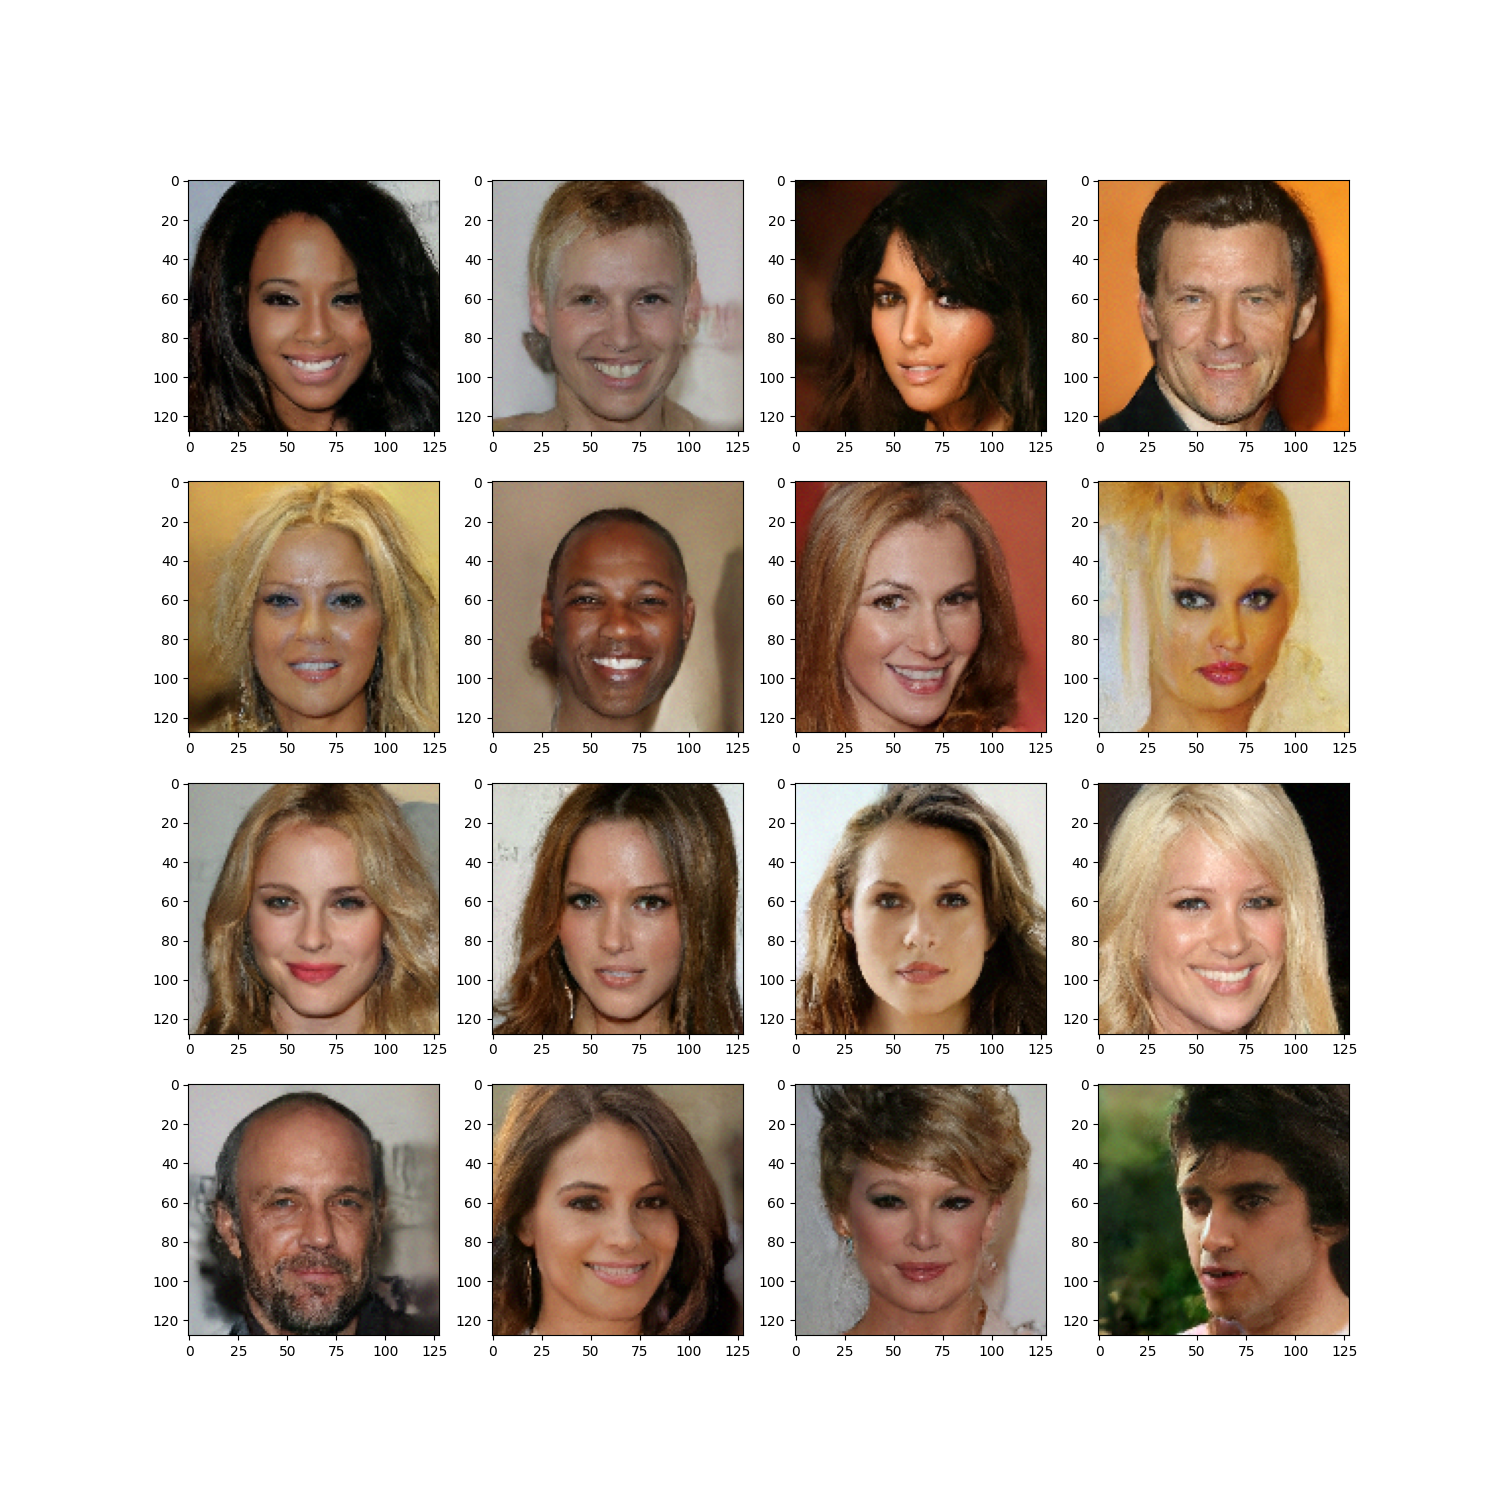
\includegraphics[width=16cm, height = 16cm]{sde_model_1000.png}
    \caption{Figure shows images generated by VP model.}
\label{fig:vp_example}
\end{figure}

\begin{figure}[H]
\hspace*{-2cm}  
    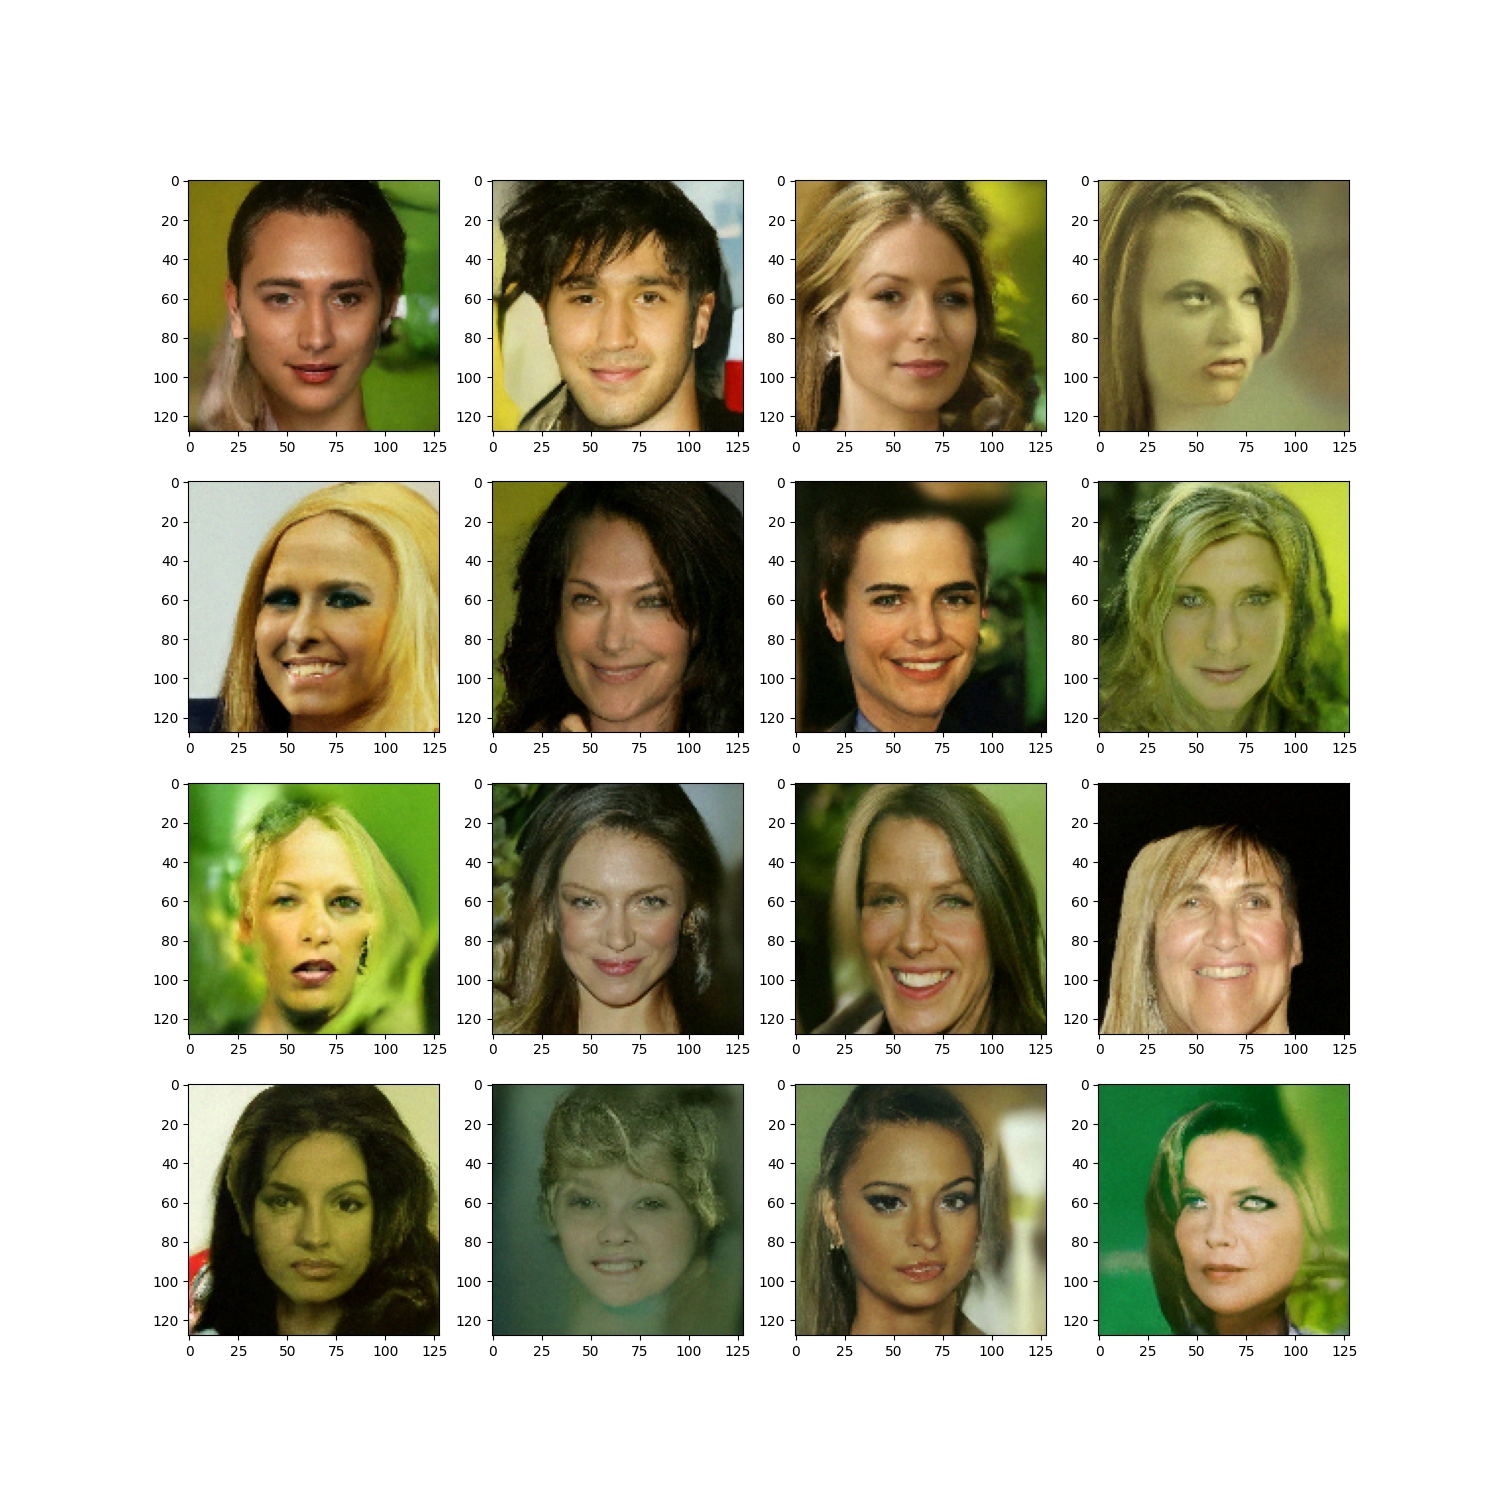
\includegraphics[width=16cm, height = 16cm]{ve_sde.png}
    \caption{Figure shows images generated by VE model.}
\label{fig:ve_example}
\end{figure}


\section{Conclusion}

We succeeded in deriving and proving many of the most important discoveries in the domain of deep learning methods for image generation. We defined the most important algorithms, that allow for training and sampling. We derived variational autoencoders, diffusion models and score models. We also used stochastic differential equations to define image perturbation stochastic process. Additionally models were implemented, trained and sampled in order to prove, that derived equations work in practice. Thus the goal of this master's thesis was accomplished.

\subsection{Further research}
The most obvious direction to improve presented results would be to increase both resolution of images and size of used models. Aside of image quality, the most important research direction is increase in output control. Example of improved controllability of the models would be conditioning them on text, which is implemented by extension of diffusion model called Stable Diffusion \cite{stable_diff}\cite{SDXL}. Similarly we could try to improve score model. Combining Stable Diffusion with stochastic differential equation would be another promising direction of model improvement.

\subsection{Challenges}
We will conclude by outlining challenges that researchers of theory, implementation and computer hardware are facing. Problems will described shallowly but broadly, placed in wider context
\subsubsection{Challenges related to memory and computation}
In recent decade we have seen how important factor in model quality is it's size. Increase in neural networks size has lead us to insight that models may have emergent capabilities \cite{emergent}. GPT model evolution is great example of recent trends regarding model sizes.  GPT 3/3.5  has around 175 billion parameters(according to authors, 10 times more than any of it's predecessors), while GPT-MoE according to NVIDIA has 1.8 trillion parameters (\cite{nvidia_gtc} at 21:46). 

Said models, were trained on internet archives. Increase in required computational capabilities of hardware is very large. Image generation models follow similar, although on smaller scale, direction. Good example in the field of image generation is SDXL \cite{SDXL} that in total has around 3.5 billion parameter. In order to obtain models that can be versatile, it is required to train those models on large datasets like LION-5B or LION-400M \cite{lion_dataset}. Such a big models and datasets can be processed only on sufficiently fast hardware.

It is important to separate data processing on two parts that is training and inference. During training 
in order to process large data volumes we care mostly about throughput. During inference, depending on the task, we need to balance throughput and latency (for example, autonomous vehicle should have shortest latency possible because we care about reaction time the most). Additionally power consumption by servers used for training or inference is very large, what generates economical and environmental costs and limits practical applications of deep learning models. 

To sum up, hardware manufacturers are facing challenge of creating hardware that is both fast and energy efficient. The fact that deep learning computation is mostly related to basic mathematical operations, matrix multiplications and data manipulation combined with the need for speed and efficiency, might be stimulus that will create new type of hardware, that is accelerators that specialize in deep learning applications.
\subsubsection{Theoretical and implementation challenges}
One of the most fundamental factors that limits effectiveness of deep learning models is the fact that gradient is local operator and impossibility, in general, to write loss function as a convex function. Result of those two limiting factors is optimization process that has "closed eyes", that means we are unable to create path that always leads us to global minimum. At the moment of writing this publication we we cannot be sure where global optimum lies, we cannot even outline area where global optimum is located.

Related to the previous limitation, is lack of possibility to check if achieving global optimum will yield satisfactory results. Fortunately, the empirical results are showing that despite of those limitations, models can achieve satisfactory results although those results might be achieved in highly unoptimal way. 

Another fundamental problem is lack of knowledge regarding deep learning model interpretation. There are some methods that can give clues and leads regarding functionality of certain neurons, but at this moment there is no method that can make role of every neuron interpretable. Those limitations are cause of many funds being wasted on models, that could not work and forces us to use brute force methods for training and model selection. Lack of interpretability of deep learning models undermines their credibility in eyes of wider audience  and limits applications in high-risk activities (who would like to fly autonomous airplane that crashes due undefined behaviour caused by small fluctuation in input data).

Based on empirical results it is worth to mention optimizers that stabilize and accelerate training process. Question whether there are undiscovered optimizers that can significantly improve training process remains open. 

Regarding problems that are less fundamental, it is worth to mention existence of matrix multiplication(in particular for sparse matrices) that are more efficient computationally- or memory- wise. Algorithm that improves computation of attention mechanism in transformers \cite{transformery} would have big impact on whole deep learning landscape (at the time of writing this publication retentive network \cite{ret_net} has been proposed as a substitute, however there is lack of empirical data to evaluate it). An equally important issue is how to achieve emergent capabilities of large models with smaller ones. An attempt was made to resolve this in the \cite{liquid_net} by proposing liquid networks. Liquid networks combine neural networks with differential equations. They are worth mentioning because they are kind of generalization of one of the biggest breakthroughs in second decade of 21st century that is skip/shortcut connection  \cite{resnet_block}.

\subsection{Summary}
Problems mentioned above are, according to the author at the time of writing, one of the most important problems, however not the only ones what is worth to point out.  Furthermore, by reviewing progress of recent decades and pace of deep learning landscape change, it is important to keep mind open to novelty and awareness that many of mentioned problems might be either solved or replaced by another ones.

\bibliography{bibliography.bib}
\bibliographystyle{unsrt}
\nocite{*}
\end{document}